%%%%%%%%%%%%%%%%%%%%%%%%%%%%%%%%%%%%%%%%%%%%%%%%%%%%%%%%%%%%%%%%%%%%%%%%%%%%%%%%
%% 
%%%%%%%%%%%%%%%%%%%%%%%%%%%%%%%%%%%%%%%%%%%%%%%%%%%%%%%%%%%%%%%%%%%%%%%%%%%%%%%%

\documentclass[a4paper, 12pt, oneside]{book}

%%-- Geometría principal (dejar activada la siguiente línea en la versión final)
\usepackage[a4paper, left=2.5cm, right=2.5cm, top=3cm, bottom=3cm]{geometry}
%%-- Activar esta línea y comentar la anterior en modo borrador, para comentarios al margen
%\usepackage[a4paper, left=2.5cm, right=2.5cm, top=3cm, bottom=3cm, marginparwidth=60pt]{geometry}

%%-- Hay que cargarlo antes que las traducciones
\usepackage{listing}                    % Listados de código

% Traducciones en XeLaTeX
% \usepackage{polyglossia}
%\setmainlanguage{spanish}    % Comenta esta línea si tu memoria es en inglés

% Traducciones particulares para español
% Caption tablas
%\gappto\captionsspanish{
%	\def\tablename{Tabla}
%	\def\listingscaption{Código}
%	\def\refname{Bibliografía}
%	\def\appendixname{Apéndice}
%	\def\listtablename{Índice de tablas}
%	\def\listingname{Código}
% 	\def\listlistingname{Índice de fragmentos de código}
%}

%% Tipografía y estilos
\usepackage[OT1]{fontenc}               % Keeps eulervm happy about accents encoding

% Símbolos y fuentes matemáticas elegantes: Euler virtual math fonts
% ¡Importante! Carga siempre las fuentes math AMS Euler ANTES QUE fontspec
\usepackage{amsmath}
\usepackage{amssymb}
\usepackage[OT1,euler-digits,euler-hat-accent,small]{eulervm}

% En XeLaTeX las fuentes se especifican con fontspec
\usepackage{fontspec}
\defaultfontfeatures{Scale=MatchLowercase, Ligatures=TeX}     % Default option in font config

% Fix para fuentes usadas con operadores y \mathrm
\DeclareSymbolFont{operators}{\encodingdefault}{\familydefault}{m}{n}

% Configura la fuente principal (serif): MinionPro
\setmainfont[Scale=0.96]{TeX Gyre Pagella}
% Configura la fuente sans-serif (\sffamily)
\setsansfont[Scale=MatchLowercase]{Lato}
% Configura la fuente para letra monoespaciada: Source Code Pro, escala 0.85
\setmonofont[Scale=0.85]{Source Code Pro}

%%-- Familias de fuentes específicas
%%-- Se pueden definir etiquetas para familias de fuentes personalizadas
%%-- que luego puedes emplear para cambiar el formato de una parte de texto
%%-- Ejemplo:
% \newfontfamily{\myriadprocond}{Myriad Pro Semibold Condensed.otf}

%%-- Opciones de interlineado y espacios
\linespread{1.07}                   % Aumentar interlineado para fuentes tipo Palatino
\setlength{\parskip}{\baselineskip} % Separar párrafos con línea en blanco

%%-- Hipervínculos
\usepackage{url}

%%-- Gráficos y tablas
\PassOptionsToPackage{dvipdfmx,usenames,dvipsnames,x11names,table}{xcolor}             % Definiciones de colores
\PassOptionsToPackage{xetex}{graphicx}

\usepackage{subfig}                     % Subfiguras
\usepackage{pgf}
\usepackage{svg}                        % Integración de imágenes en formato SVG
\usepackage{float}                      % H para posicionar figuras
\usepackage{booktabs}                   % Already loads package xcolor
\usepackage{multicol}                   % multiple column layout facilities
\usepackage{colortbl}                   % For coloured tables

%%-- Bibliografía con Biblatex y Biber
% Más info:
% https://www.overleaf.com/learn/latex/Biblatex_bibliography_styles
% https://www.overleaf.com/learn/latex/biblatex_citation_styles
\usepackage[british]{babel}
\usepackage[
    style=numeric,
    sorting=none
    ]{biblatex}
\addbibresource{memoria.bib}
% \DeclareFieldFormat{url}{\mkbibacro{URL}\addcolon\nobreakspace\url{#1}}
%\usepackage[nottoc, notlot, notlof, notindex]{tocbibind} %% Opciones de índice

%%-- Matemáticas e ingeniería
% El paquete units permite mostrar unidades correctamente
% Permite escribir unidades con espaciado y estilo de fuente correctos
\usepackage{units}         
% Ejemplo de uso: $\unit[100]{m}$ or $\unitfrac[100]{m}{s}$
% Entornos matemáticos
\newtheorem{theorem}{Theorem}

% Paquetes adicionales
\usepackage{url}                        %% Gestión correcta de enlaces
\usepackage{float}                      %% H para posicionar figuras
\usepackage[nottoc, notlot, notlof, notindex]{tocbibind}    %% Opciones de índice
\usepackage{metalogo}                   %% Múltiples logos para XeLaTeX

% Fuentes especiales y glifos
\usepackage{ccicons}                % Creative Commons icons
\usepackage{metalogo}               % XeTeX logo
\usepackage{fontawesome5}           % Fontawesome 5 icons
\usepackage{adforn} 

% Blindtext
% Opciones pangram, bible, random (defecto)
\usepackage[pangram]{blindtext}
% Lorem ipsum
\usepackage{lipsum}
% Kant lipsum
\usepackage{kantlipsum}

\usepackage{fancyvrb}               % Entornos verbatim extendidos
	\fvset{fontsize=\normalsize}    % Tamaño de fuente por defecto en fancy-verbatim
	
% Configura listas (itemize, enumerate) con iconos personalizados
% Fácil reinicio de numeración con enumerate
% Info: http://ctan.org/pkg/enumitem
\usepackage[shortlabels]{enumitem}
% Usar \usageitem para configurar iconos personalizados en listas
\newcommand{\usageitem}[1]{%
	\item[%
	{\makebox[2em]{\strut\color{GSyCblue} #1}}%
	]
}

%%-- Definición de colores personalizados
% \definecolor{LightGrey}{HTML}{EEEEEE}
% \definecolor{darkred}{rgb}{0.5,0,0}     %% Refs. cruzadas
% \definecolor{darkgreen}{rgb}{0,0.5,0}   %% Citas bibliográficas
% \definecolor{darkblue}{rgb}{0,0,0.5}    %% Hiperenlaces ordinarios (también ToC)

%%-- Configuración fragmentos de código
%%-- Minted necesita Python Pygments instalado en el sistema para funcionar
%%-- En Overleaf ya está instalada esta dependencia
\usepackage[labelfont=bf]{caption}
\newcommand{\source}[1]{\vspace{-3pt} \caption*{Source: {#1}} }
\usepackage{minted}
\usemintedstyle{vs}

%%-- Se debe cargar aquí para evitar warnings
\usepackage{csquotes}                   % Para traducciones con biblatex

%%-- Glosario de términos
\usepackage[acronym]{glossaries}
\makeglossaries
\loadglsentries{glossary}

% % Definición de cabeceras del documento, usando fancyhdr
% \usepackage{fancyhdr}
% %% Configuración de cabeceras para el cuerpo principal del documento
% \pagestyle{fancy}
% \fancyhead{}
% \fancyhead[RO,LE]{\myriadprocond{\thepage}}
% \renewcommand{\chaptermark}[1]{\markboth{\chaptername\ \thechapter.\ #1}{}}
% \renewcommand{\sectionmark}[1]{\markright{\thesection.\ #1}}
% \fancyhead[RE]{\myriadprocond{\leftmark}}
% \fancyhead[LO]{\myriadprocond{\rightmark}}
% \renewcommand{\headrulewidth}{0pt}
% \setlength{\headheight}{15pt} %% Al menos 15pt para evitar warning al compilar
% \fancyfoot{}
% %% Configuración para páginas con cabecera en blanco
% \fancypagestyle{plain}{%
% \fancyhf{}% clear all header and footer fields
% \fancyhead[RO,LE]{\myriadprocond{\thepage}}
% \renewcommand{\headrulewidth}{0pt}%
% \renewcommand{\footrulewidth}{0pt}%
% }
\AtBeginDocument{\addtocontents{toc}{\protect\thispagestyle{empty}}} 

%%%%%%%%%%%%%%%%%%%
%% Own changes
%%%%%%%%%%%%%%%%%%%
\newenvironment{conditions}[1][where:]
  {#1 \begin{tabular}[t]{>{$}l<{$} @{${}={}$} l}}
  {\end{tabular}\\[\belowdisplayskip]}
\raggedbottom


%%%%%%%%%%%%%%%%%%%%%%%%%%%%%%%%%%%%%%%%

%%-- Metadatos del doc
\title{Exploration of vision-based control solutions for PX4-driven UAVs}
\author{Laura Gonzalez Fernandez}

%%-- Hiperenlaces, siempre se carga al final del preámbulo
\usepackage[colorlinks]{hyperref}
\hypersetup{
    pdftoolbar=true,	% Muestra barra de herramientas en Adobe Acrobat
	pdfmenubar=true,	% Muestra menú en Adobe Acrobat
	pdftitle={TFG - Exploration of vision-based control solutions for PX4-driven UAVs},
	pdfauthor={Laura Gonzalez Fernandez},
	pdfcreator={ETSIT, URJC},
	pdfproducer={XeLaTeX},
	pdfsubject={UAV, PX4, control},
	pdfnewwindow=true,              %links open in new window
    colorlinks=true,                % false: boxed links; true: coloured links
    linkcolor=Firebrick4,           % enlaces internos 
    citecolor=Aquamarine4,          % enlaces a citas bibliográficas
    urlcolor=RoyalBlue3,            % hiperenlances ordinarios
    linktocpage=true                % Enlaces en núm. pág. en ToC
}

%%%---------------------------------------------------------------------------
% Comentarios en línea de revisión
% Este bloque se puede borrar cuando finalizamos el borrador

\usepackage[colorinlistoftodos]{todonotes}
\usepackage{verbatim}

% \hyphenpenalty 10
% \exhyphenpenalty 10
\pretolerance=5000
\tolerance=9000
\emergencystretch=2pt
\righthyphenmin=4
\lefthyphenmin=4

\interfootnotelinepenalty=10000

\usepackage[
    type={CC},
    modifier={by-sa},
    version={4.0},
]{doclicense}

%%%---------------------------------------------------------------------------

\begin{document}

%%-- Configuración común para todos los entornos listing
%%-- Descomentar para usar y personalizar valores
%\lstset{%
%breakatwhitespace=true,
% breaklines=true, 
% basicstyle=\footnotesize\ttfamily,
% keywordstyle=\color{blue},
% commentstyle=\color{green!40!black}, 
% language=Python} 
 

%%%%%%%%%%%%%%%%%%%%%%%%%%%%%%%%%%%%%%%%%%%%%%%%%%%%%%%%%%%%%%%%%%%%%%%%%%%%%%%%
% PORTADA

\begin{titlepage}
\begin{center}
\begin{tabular}[c]{c c}
%\includegraphics[bb=0 0 194 352, scale=0.25]{logo} &
\includegraphics[scale=1.5]{img/LogoURJC.png}
%&
%\begin{tabular}[b]{l}
%\Huge
%\textsf{UNIVERSIDAD} \\
%\Huge
%\textsf{REY JUAN CARLOS} \\
%\end{tabular}
\\
\end{tabular}

\vspace{3cm}

\Large 
GRADO EN INGENIERÍA AEROESPACIAL EN AERONAVEGACIÓN

\vspace{0.4cm}

\large
Curso Académico 2023/2024

\vspace{0.8cm}

Trabajo Fin de Grado

\vspace{2cm}

\LARGE Exploration of vision-based \\
control solutions for PX4-driven UAVs
\vspace{3cm}

\large
Autora : Laura González Fernández \\
Tutores : Xin Chen, Alejandro Sáez Mollejo
\end{center}
\pagenumbering{gobble}
\end{titlepage}

\newpage
\mbox{}


%%%%%%%%%%%%%%%%%%%%%%%%%%%%%%%%%%%%%%%%%%%%%%%%%%%%%%%%%%%%%%%%%%%%%%%%%%%%%%%%
%%%% Para firmar
\clearpage
\frontmatter
\pagestyle{empty}
\chapter*{}
\thispagestyle{empty}

\vspace{-4cm}
\begin{center}
\LARGE
\textbf{Trabajo Fin de Grado}

\vspace{1cm}
\large
Exploration of Vision-Based Control Solutions for PX4-Driven UAVs.

\vspace{1cm}
\large
\textbf{Autora :} Laura González Fernández \\
\textbf{Tutores :} Xin Chen, Alejandro Sáez Mollejo

\end{center}

\vspace{1cm}
La defensa del presente Proyecto Fin de Grado se realizó el día \qquad$\;\,$ de \qquad\qquad\qquad\qquad \newline de 2023, siendo calificada por el siguiente tribunal:


\vspace{0.5cm}
\textbf{Presidente:}

\vspace{0.8cm}
\textbf{Secretario:}

\vspace{0.8cm}
\textbf{Vocal:}


\vspace{0.8cm}
y habiendo obtenido la siguiente calificación:

\vspace{0.8cm}
\textbf{Calificación:}


\vspace{0.8cm}
\begin{flushright}
Fuenlabrada, a \qquad$\;\,$ de \qquad\qquad\qquad\qquad de 2023
\end{flushright}

%%%%%%%%%%%%%%%%%%%%%%%%%%%%%%%%%%%%%%%%%%%%%%%%%%%%%%%%%%%%%%%%%%%%%%%%%%%%%%%%
%%%% Dedicatoria

% \chapter*{}
% \thispagestyle{empty}
% %\pagenumbering{Roman} % para comenzar la numeración de paginas en numeros romanos
% \begin{flushright}
% \textit{To the future.\\}
% \end{flushright}

\chapter*{}
\thispagestyle{empty}
%\pagenumbering{Roman} % para comenzar la numeración de paginas en numeros romanos

\begin{flushright}
\begin{minipage}{8cm}
\raggedleft
©2023 Laura González Fernández  \\
Some rights reserved. \\
\doclicenseLongText \\
\vspace{0.5cm}
\doclicenseImage
\end{minipage}

\end{flushright}

%%%%%%%%%%%%%%%%%%%%%%%%%%%%%%%%%%%%%%%%%%%%%%%%%%%%%%%%%%%%%%%%%%%%%%%%%%%%%%%%
%%%% Agradecimientos

\chapter*{Acknowledgements}
\thispagestyle{empty}
%\addcontentsline{toc}{chapter}{Agradecimientos} % si queremos que aparezca en el índice
\markboth{ACKNOWLEDGEMENTS}{ACKNOWLEDGEMENTS} % encabezado 

I would like to take this opportunity to express my deepest gratitude to the many individuals who have played a significant role in the completion of this bachelor thesis.

First and foremost, I want to thank my family for their unwavering support and patience throughout my academic journey. They never doubted me, even when I did it myself. Thank you as well for your help during this project, for being there when I needed a camera person or an extra hand to fly the drone. To my sister, especially, thank you for putting up with me these two years while I inched along this project.

I also extend my thanks to my supervisors for their guidance, expertise, and invaluable feedback throughout the thesis project. Your dedication to my academic growth and your willingness to share your knowledge have been indispensable.

I would also like to express my gratitude to all my friends and colleagues who were by my side during this journey. Your camaraderie and the frequent inquiries about the status of my "never-ending drone project" pushed me towards the finish line.

This thesis represents the culmination of years of hard work and dedication, and I am grateful for the support of everyone who stood by my side.

Thank you all for being a part of this journey.

%%%%%%%%%%%%%%%%%%%%%%%%%%%%%%%%%%%%%%%%%%%%%%%%%%%%%%%%%%%%%%%%%%%%%%%%%%%%%%%%
%%%% Resumen

\chapter*{Resumen}
\thispagestyle{empty}
%\addcontentsline{toc}{chapter}{Resumen} % si queremos que aparezca en el índice
\markboth{RESUMEN}{RESUMEN} % encabezado

La popular plataforma de código abierto PX4 surge con el objetivo de facilitar el desarrollo de nuevas soluciones para vehículos aéreos no tripulados y su integración con nuevas tecnologías para favorecer su acercamiento al público general. Esta tesis pretende demonstrar cómo esta plataforma puede ser empleada para desarrollar y evaluar estrategias de control que integren técnicas de visión artificial existentes, utilizando sus resultados para controlar el movimiento de un vehículo aéreo y empleando componentes electrónicos de bajo presupuesto. Para mostrar las capacidades de las herramientas disponibles, se presenta un método de control viable que permite a un dron usar una cámara abordo del mismo para identificar y realizar un seguimiento de una persona en su campo de visión, cuyos movimientos son reflejados por el vehículo.

%%%%%%%%%%%%%%%%%%%%%%%%%%%%%%%%%%%%%%%%%%%%%%%%%%%%%%%%%%%%%%%%%%%%%%%%%%%%%%%%
%%%% Resumen en inglés

\chapter*{Abstract}
\thispagestyle{empty}
%\addcontentsline{toc}{chapter}{Summary} % si queremos que aparezca en el índice
\markboth{ABSTRACT}{ABSTRACT} % encabezado

The popular open-source platform PX4 aims to facilitate the development and integration of new solutions for unmanned aerial vehicles, making them approachable for the common developer. This thesis aims to demonstrate how this platform can be used to develop and test control strategies that integrate existing computer vision techniques, using their input to control the movement of an aerial vehicle while employing readily available and affordable hardware components with basic specifications. To showcase the tools available, a viable solution is presented that allows a drone to use an onboard camera to identify and keep track of a person in its field of view to follow their movement.

%%%%--------------------------------------------------------------------
% Lista de comentarios de revisión
% Se puede borrar este bloque al acabar el borrador

% \listoftodos
% \thispagestyle{empty}
% \markboth{TODO LIST}{TODO LIST} % encabezado
%%%%--------------------------------------------------------------------

%%%%%%%%%%%%%%%%%%%%%%%%%%%%%%%%%%%%%%%%%%%%%%%%%%%%%%%%%%%%%%%%%%%%%%%%%%%%%%%%
%%%%%%%%%%%%%%%%%%%%%%%%%%%%%%%%%%%%%%%%%%%%%%%%%%%%%%%%%%%%%%%%%%%%%%%%%%%%%%%%
% ÍNDICES %
%%%%%%%%%%%%%%%%%%%%%%%%%%%%%%%%%%%%%%%%%%%%%%%%%%%%%%%%%%%%%%%%%%%%%%%%%%%%%%%%

% Las buenas noticias es que los índices se generan automáticamente.
% Lo único que tienes que hacer es elegir cuáles quieren que se generen,
% y comentar/descomentar esa instrucción de LaTeX.

%%-- Índice de contenidos
\tableofcontents 
\thispagestyle{empty}
\cleardoublepage
%%-- Índice de figuras

\addcontentsline{toc}{chapter}{List of figures} % para que aparezca en el indice de contenidos
\thispagestyle{empty}
\listoffigures % indice de figuras
\thispagestyle{empty}

\cleardoublepage
%%-- Índice de tablas
%\addcontentsline{toc}{chapter}{Lista de tablas} % para que aparezca en el indice de contenidos
%\listoftables % indice de tablas
% \cleardoublepage
%%-- Índice de fragmentos de código
% \addcontentsline{toc}{chapter}{List of listings} % para que aparezca en el indice de contenidos
% \listoflistings

%%%%%%%%%%%%%%%%%%%%%%%%%%%%%%%%%%%%%%%%%%%%%%%%%%%%%%%%%%%%%%%%%%%%%%%%%%%%%%%%
%%%%%%%%%%%%%%%%%%%%%%%%%%%%%%%%%%%%%%%%%%%%%%%%%%%%%%%%%%%%%%%%%%%%%%%%%%%%%%%%
%%%%%%%%%%%%%%%%%%%%%%%%%%%%%%%%%%%%%%%%%%%%%%%%%%%%%%%%%%%%%%%%%%%%%%%%%%%%%%%%
%%%%%%%%%%%%%%%%%%%%%%%%%%%%%%%   CONTENT   %%%%%%%%%%%%%%%%%%%%%%%%%%%%%%%%%%%%
%%%%%%%%%%%%%%%%%%%%%%%%%%%%%%%%%%%%%%%%%%%%%%%%%%%%%%%%%%%%%%%%%%%%%%%%%%%%%%%%
%%%%%%%%%%%%%%%%%%%%%%%%%%%%%%%%%%%%%%%%%%%%%%%%%%%%%%%%%%%%%%%%%%%%%%%%%%%%%%%%
%%%%%%%%%%%%%%%%%%%%%%%%%%%%%%%%%%%%%%%%%%%%%%%%%%%%%%%%%%%%%%%%%%%%%%%%%%%%%%%%
\mainmatter
\pagestyle{headings}

% INTRODUCTION %
\cleardoublepage
\chapter{Introduction}
\label{sec:intro}
\pagenumbering{arabic} % para empezar la numeración de página con números

\section{General context}

% An Unmanned Aerial Vehicle (UAV) is an aircraft able to fly without any pilot or operator on board. They may be operated through remote control by a human operator or with various degrees of autonomy, from sensor-driven control aids provided to the operator to fully autonomous flight through preplanned missions.
% UAVs have existed since the 20th century and were initially developed as military technology to protect pilots from dangerous missions.
% However, as the cost of the electronics and sensors decreased and control technologies improved, they became available to a broader public. They are now employed in various civil applications like crop control, search and rescue, or filmmaking and photography.
% Most commercial solutions are limited to remote operations or rudimentary autonomy, with fully autonomous flight still in the earliest phases.
% However, there is a growing trend towards using vision-based control solutions, which can offer improved performance and flexibility compared to traditional control methods.

% Vision-based control solutions use cameras and image processing algorithms to provide real-time feedback and control of the UAV. 
% These solutions are often more flexible and robust than traditional control methods, which are typically based on accelerometers, gyroscopes, and other sensors. 
% Additionally, vision-based control solutions can be implemented on low-cost platforms, making them accessible to a broader range of users.
% These vision-based guidance systems have only started to appear in recent years as artificial intelligence becomes more widespread and very few fully-developed consumer-ready platforms are available for the general public.
% Even so,
% from the essential hardware to build an own quadcopter, a helicopter with four rotors that represents the most common type of UAV, to miniaturized computers that handle complex calculations and open-source software that can be customized to endless applications,
% all the individual pieces that enable building such a system are readily available.

Unmanned Aerial Vehicles (UAVs), commonly known as drones, have emerged as remarkable aircraft capable of flying without a pilot or operator on board. Originally developed as military technology to safeguard pilots from dangerous missions, UAVs have transitioned into the civilian domain due to advancements in control technologies and the decreasing costs of electronics and sensors. This has led to broader accessibility of UAVs, allowing their utilization in diverse civil applications such as crop monitoring, search and rescue operations, and filmmaking and photography.
Traditionally, UAVs have been operated either remotely by a human operator or with limited autonomy through preplanned missions. However, recent trends have indicated a shift towards vision-based control solutions, which offer promising advantages over conventional control methods. Vision-based control harnesses the power of cameras and image processing algorithms to provide real-time feedback and precise control of UAVs.

Compared to traditional control systems that heavily rely on sensors such as accelerometers and gyroscopes, vision-based control solutions offer greater flexibility and robustness. By leveraging the visual input from cameras, these solutions can adapt to varying environmental conditions and handle complex flight scenarios more effectively. Furthermore, vision-based control methods are often more accessible, as they can be implemented on lower-cost platforms, making them appealing to a wider range of users.
While the integration of vision-based control solutions into UAVs is a relatively recent development, propelled by the increasing prevalence of artificial intelligence, there is limited availability of fully-developed consumer-ready platforms in the market. However, this does not impede progress in this field, as all the necessary components for constructing such systems are readily available. From the essential hardware required to build a quadcopter, which represents the most common type of UAV, to miniaturized computers capable of handling complex calculations, and open-source software that can be customized for endless applications, the individual pieces required for constructing and implementing vision-based control solutions are very accessible.

In summary, the rise of UAVs and their integration into various civil applications has paved the way for the exploration of vision-based control solutions. These solutions, utilizing cameras and image processing algorithms, offer enhanced performance, adaptability, and accessibility compared to traditional control methods. Although consumer-ready platforms are still emerging, the necessary components for constructing vision-based control systems are readily available, fueling the advancement of this field.

\section{The drone-vision-control project}

\todo[inline]{Rename everything to VisionFlight ??}

% The project presented in this thesis aims to show the tools available to design and implement control solutions for the popular PX4 open-source autopilot platform and how to integrate them with detection and tracking computer vision mechanisms to achieve simple vision-based self-guided UAVs.
% To do that, a simple application has been developed to use as a basis for delving into the PX4 ecosystem and exploring ways of integrating the hardware and software necessary to control a UAV.
% Two main architectures of software and hardware interaction in vision-based scenarios are proposed based on whether the vision module is located offboard or onboard the vehicle during flight.
% The first case, the simpler of the two, will be used as a landing platform to begin development and test the most basic integration between the tools employed, by designing a proof-of-concept control mechanism that translates hand gestures executed in front of an independent camera to flight commands that control the movement of the vehicle.
% The second scenario builds upon the previous one to integrate the camera and vision computation onboard the vehicle to develop a tracking and following control solution that looks for a person standing in the field of view of the drone and mirrors its movements in a 3D environment to keep it on sight.

% This thesis explores the development environment used, which enables a process for designing the software in a way that gradually adapts to the hardware employed by building up progressively from a completely simulated flight controller to actual flight tests in an unmanned vehicle.
% To do that, the AirSim simulation engine is leveraged to build an environment that allows for safe and thorough testing of unreliable, in-progress control solutions.
% All the necessary code for this project has been written in Python and always runs outside the flight controller board on a companion computer.
% This allows more processing power to be accessible for any compute-intensive computer vision algorithms,
% but also ensures that the control solutions are abstracted from the hardware components and not dependent on the specific flight stack employed, 
% to allow applying the results to any available autopilot platform with exposed APIs.

The project outlined in this thesis is a comprehensive exploration of the tools available for designing and implementing control solutions for the PX4 open-source autopilot platform. The goal is to demonstrate how these tools can be integrated with computer vision mechanisms to achieve vision-based self-guided unmanned aerial vehicles (UAVs).
To achieve this objective, a simple application has been developed, named Drone Vision Control serving as a foundation for the investigation into the PX4 ecosystem and methods of integrating the necessary hardware and software for UAV control.
For the computer vision detection mechanisms, the ready-to-use Mediapipe suite of libraries for real-time image analyses on hand-held devices has been employed to reduce the complexity of the project.
Two primary architectures for integrating software and hardware in vision-based scenarios have been proposed, with one scenario involving off-board vision modules and the other integrating onboard camera and vision computation. 

The first scenario involves a proof-of-concept control mechanism that translates hand gestures executed in front of an independent camera to flight commands, thereby controlling the movement of the vehicle. This serves as a landing platform to begin development and test the most basic integration between the tools employed.
The second scenario builds on the first to integrate the camera and vision computation onboard the vehicle to develop a tracking and following control solution that can track and follow a person standing in the drone's field of view by mirroring their movements in a 3D environment.

To further the development of these control mechanisms, a dedicated development environment was employed. This environment facilitated the design process by allowing a gradual adaptation of the software to match the hardware requirements, starting from a purely simulated flight controller and progressing towards real flight tests in an unmanned vehicle.
The key component of this environment is the integration with the AirSim simulation engine. Built upon the powerful 3D computer graphics game engine Unreal, it provides a platform that ensures secure and comprehensive testing of control solutions that are still in progress and not yet fully reliable.

For this project, all the code has been implemented in Python, running on a companion computer separate from the flight controller board. This deliberate approach ensures that the control solutions remain independent of the hardware components and are not tied to any particular flight stack. Consequently, the results obtained can be applied to any autopilot platform that offers exposed APIs and are not limited to the PX4 ecosystem. 

In conclusion, this thesis offers a thorough investigation into the development of vision-based self-guided UAVs, presenting a range of tools and techniques that can be utilized to accomplish this objective.

\section{Objectives}
\label{sec:objetives}

The main objective of this project is to explore the tools and methods available for designing and implementing control solutions for the PX4 open-source autopilot platform and demonstrate how they can be integrated with computer vision mechanisms to achieve a self-guided UAV that tracks and follows a person's movements.

More specifically, it aims to:
\begin{itemize}
    % \item Introduce the software and hardware environment of the Dronecode project and the techniques they have made available.
    % \item Show the minimum requirements needed to develop control software for the platform.
    % \item Suggest viable vision-driven control solutions that use those techniques.
    % \item Present a testing process using available tools that can help ensure safety and reliability for any new solutions developed.
    % \item Build a quadcopter and use it to carry out test flights with the developed solutions.
    \item Research and understand the PX4 platform and its wider ecosystem, including its architecture, capabilities, and available APIs.
    \item Explore existing computer vision mechanisms and algorithms suitable for vision-based control of UAVs.
    \item Design and set up a dedicated development environment using the AirSim simulation engine for secure and comprehensive testing of control solutions.
    \item Employ both software-in-the-loop and hardware-in-the-loop simulation approaches to comprehensively evaluate the control solutions in the simulation engine.
    \item Develop a proof-of-concept control mechanism that translates hand gestures captured by a camera into flight commands for the UAV.
    \item Integrate the hand gesture control mechanism with the PX4 platform and test its functionality in a simulated environment.
    \item Investigate hardware and software requirements for integrating onboard cameras and vision computation in UAVs.
    \item Develop a tracking and following control solution that can mirror the movement of a person.
    \item Test the tracking and following control solution in a simulated environment, integrating the onboard camera and vision computation with the PX4 platform.
    \item Conduct flight tests on a self-built quadcopter to evaluate the developed control mechanisms, analyzing their performance and reliability in different scenarios.
    \item Document the findings, methodologies, and results obtained throughout the project and provide recommendations for future improvements.
\end{itemize}


\section{Time planning}
\label{sec:time-planning}

\begin{figure}
  \centering
  \makebox[\textwidth][c]{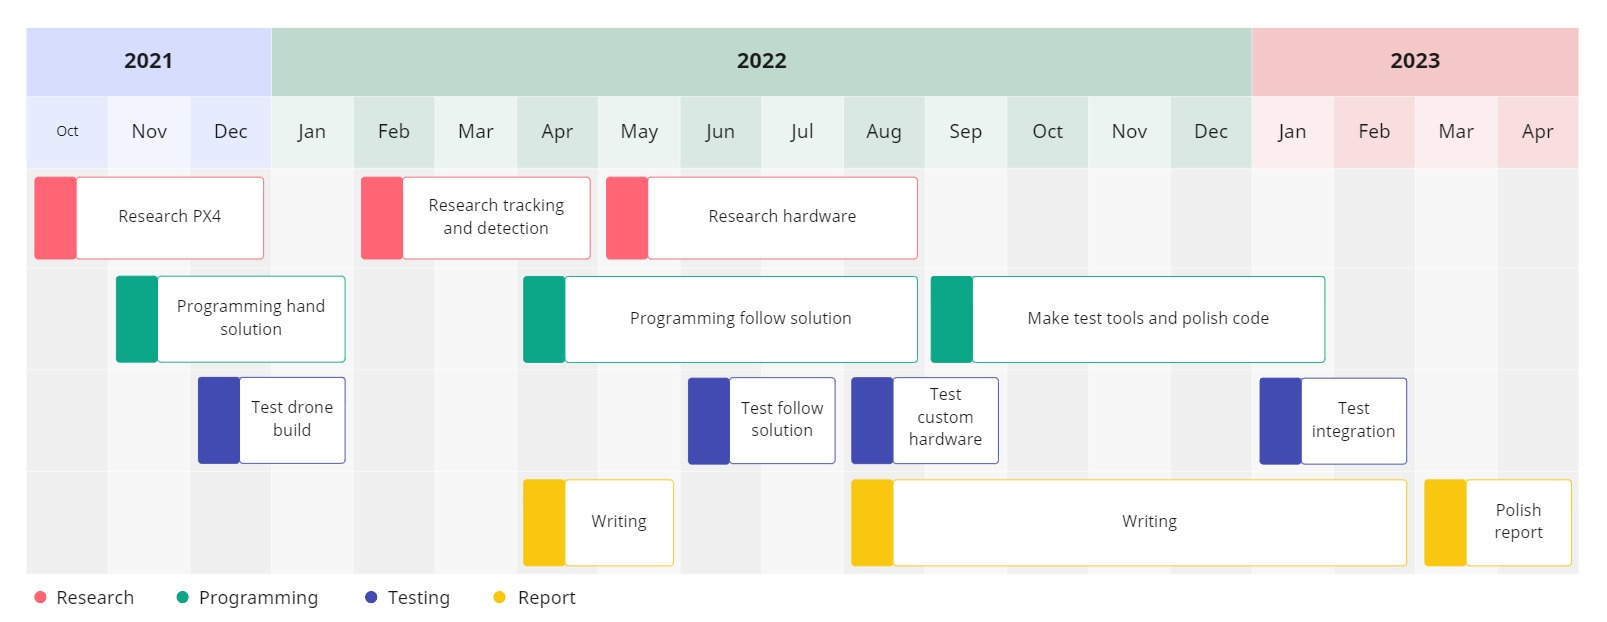
\includegraphics[width=1.1\textwidth,keepaspectratio]{img/project-timeline.jpg}}
  \caption{Timeline for the development of the project}
  \label{fig:project-timeline}
\end{figure}

% This project has been carried out over a natural period of one and a half years due to having to coordinate with working a full-time job in parallel.
% The development has been spread out over three phases, taking up a total of 400 hours of dedication to the project.
% Each of these phases can be divided into three main tasks: research of the necessary systems, programming of custom solutions and tools, and comprehensive testing on different scenarios.
% Additionally, during the last two phases, time was allocated to the process of writing the report, which occurred concurrently with the research and development work.
% \begin{itemize}
%     \item Phase 1: Proof-of-concept ( Oct 21 - Jan 22: 61 hours )
%     \begin{itemize}
%         \item Research PX4 (12 hours)
%         \item Programming hand solution (42 hours)
%         \item Test standard drone build (7 hours)
%     \end{itemize}
%     \item Phase 2: Follow solution ( Feb 22 - Aug 22: 138 hours )
%     \begin{itemize}
%         \item Research tracking and detection (33 hours)
%         \item Programming follow solution (80 hours)
%         \item Test custom hardware (25 hours)
%     \end{itemize}
%     \item Phase 3: Hardware ( Sep 22 - Feb 23: 65 hours )
%     \begin{itemize}
%         \item Research hardware (15 hours)
%         \item Make test tools and polish code (33 hours)
%         \item Test custom hardware and integration (17 hours)
%     \end{itemize}
%     \item Writing report (133 hours)
% \end{itemize}

This project was carried out over a period of approximately one and a half years, taking into account the parallel commitment of working a full-time job. The development process was divided into three distinct phases, totalling approximately 400 hours of dedicated effort. These phases consisted of the following tasks:

\begin{itemize}
\item \textbf{Phase 1: Proof-of-concept (Oct 2021 - Jan 2022: 61 hours)}
\begin{itemize}
\item Conducted research on the PX4 system (12 hours)
\item Programmed the hand solution (42 hours)
\item Tested the standard drone build (7 hours)
\end{itemize}

\item \textbf{Phase 2: Follow solution (Feb 2022 - Aug 2022: 138 hours)}
\begin{itemize}
    \item Conducted research on tracking and detection methods (33 hours)
    \item Developed the follow solution (80 hours)
    \item Tested custom hardware (25 hours)
\end{itemize}

\item \textbf{Phase 3: Hardware (Sep 2022 - Feb 2023: 65 hours)}
\begin{itemize}
    \item Conducted research on hardware options (15 hours)
    \item Developed test tools and refined code (33 hours)
    \item Conducted testing of custom hardware and integration (17 hours)
\end{itemize}
\end{itemize}

During the initial phase, extensive research was conducted to gain a deep understanding of the PX4 system. This involved studying the architecture, capabilities, and documentation of the platform. Following the research phase, a proof-of-concept control mechanism was developed, enabling the translation of hand gestures captured by an independent camera into flight commands. Subsequently, testing was performed on the standard drone build to verify the basic integration between the control mechanism and the UAV platform.

The second phase focused on the development of an advanced tracking and following control solution. Research was conducted to explore various tracking and detection methods, including computer vision algorithms and techniques. Building upon this research, the follow solution was implemented, enabling the UAV to track and follow a person in its field of view by mirroring their movements in a 3D environment. Custom hardware components, such as sensors and actuators, were tested to ensure compatibility and reliable operation within the follow solution.

In the third phase, research was conducted to explore hardware options for the UAV system, including flight controllers, companion computers, and cameras. The chosen hardware components were integrated, and test tools were developed to enhance the performance and reliability of the control mechanisms. The system's hardware and software integration was thoroughly tested to ensure seamless operation and optimize the control algorithms.


Additionally, a significant amount of time, totalling 133 hours, was dedicated to writing the report, which was carried out concurrently with the research and development work.

This time planning and task distribution allowed for a structured approach to the project, ensuring a comprehensive exploration of the subject matter while accommodating other commitments.

\section{Thesis layout}
\label{sec:layout}

% This section details the structure of this thesis.
% It is organized into five chapters that reflect the three distinct tasks described in the last section: research, development and testing, along with this introduction and some final conclusions.
% Specifically:

% \begin{itemize}
%     \item In the first chapter, there is a brief introduction to the context in which the project has been developed, as well as the objectives it pursues.
%     \item Chapter 2 presents the technologies and tools employed in this project and the current state-of-the-art for UAV vision-based control solutions.
%     \item The third chapter introduces the simulation environments used to develop the solutions throughout the project and the architecture of the hardware and software used.
%     \item Chapter 4 follows along through the process of testing every part of the system incrementally until reaching the final flight tests.
%     \item The last chapter shows the conclusions drawn from the work and presents ideas for future development.
% \end{itemize}

The thesis is structured into five chapters, with the three main blocks focusing on each of the three specific aspects of the project mentioned in the previous section: research, development and testing. 

The first chapter serves as an introduction to the context in which the project has been developed, providing background information and highlighting the objectives pursued throughout the research. It sets the stage for the subsequent chapters, giving an overview of the project's scope and purpose.

The second chapter discusses the technologies and tools employed in the project and provides a review of the relevant literature and the current state-of-the-art for UAV vision-based control solutions.

The third chapter covers the simulation environments used throughout the project and the architecture of the hardware and software employed in the project. This chapter discusses the design decisions that went into selecting the hardware and software components and describes the overall architecture of the system.

The fourth chapter presents the testing methodology used throughout the project, from initial simulations to flight tests. This chapter provides a detailed account of the testing process and highlights the key findings and insights gained from each phase of testing.

The final chapter concludes the thesis by summarizing the key findings of the project and drawing conclusions about the effectiveness and limitations of the control system. Additionally, this chapter provides suggestions for future development and improvement of the system.

\cleardoublepage
\clearpage

% ESTADO DEL ARTE %
\chapter{State of the art}
\label{chap:sota}
\section{Literature review}
\label{sec:lit-review}

% Vision-based control solutions for UAVs on low-cost platforms have gained significant attention recently due to the increasing demand for cost-effective and efficient aerial applications. This literature review summarizes the existing research in this field and highlights the essential findings and challenges.

% A significant amount of research has focused on developing algorithms for real-time image processing, focusing on improving the accuracy and robustness of tracking solutions for UAV applications.
% In \cite{gomez-balderas2012}, a computer
% vision algorithm for position measurement and velocity estimation using optical flow is proposed for tracking ground-moving targets.
% In \cite{bevilacqua2016}, the focus is to solve the problem of tracking and following a generic human target by a drone in a natural, possibly dark scene without relying on colour information.
% In \cite{rysdyk2003}, several algorithms are developed to create path-following mechanisms that maintain a constant line of sight with the target.
% These studies attempt to develop solutions that can be applied to any platform regardless of any preexisting autopilot control in the UAVs.
% They focus on low-level software implementations of complex control theory topics with advanced mathematics.
% In contrast, this thesis aims to abstract as much as possible both the control technics and the computer vision mechanisms of detection and tracking to focus on presenting an easy-to-use platform that can employ already developed algorithms and combine them to make robust systems with a lower threshold of knowledge.

% Other studies have already centred on developing lower-cost solutions for more accessible platforms. Many have used the Parrot \emph{AR.Drone} camera-enabled quadcopter that allows controlling through WiFi from an external offboard computer.
% In \cite{bartak2015}, \cite{chakrabarty2016}, \cite{pestana2013}, and \cite{haag2015}, the \emph{AR.Drone} is used for implementing object tracking and following solutions in different environments and conditions with a higher emphasis on the type of trackers employed to achieve a robust visual following mechanism.
% In \cite{hernandez2013}, \cite{lugo2014}, and \cite{bristeau2011}, there is a higher focus on exposing the capabilities of the \emph{AR.Drone} as a platform to develop custom control solutions utilizing the navigation and control technology and the low-cost sensors already embedded in the vehicle.
% The main difference between the platform used in the mentioned research and the PX4 platform that is the target of this thesis is that the \emph{AR.Drone} is offered as-is as a concrete low-cost vehicle for which autonomous guidance and control can be developed, while the PX4 platform is part of an extensive environment that encompasses everything from the minimum essential hardware to the low-level autopilot mechanisms to the high-level control commands and allows complete personalization at each layer of the system.

% As the PX4 platform has been available for less than a decade and has only become a widely-recognized standard in the drone industry since 2020, there is still little research on its ecosystem, and fewer specific computer-vision projects have been developed.
% However, some studies share some of the possibilities that the PX4 software and the Pixhawk flight controllers offer in the field.
% In \cite{sizkouhi2022}, aerial images are analyzed in real-time and fed to a deep-learning architecture to calculate optimal flight paths.
% In \cite{naufal2022}, a vision-based precision landing method for quadcopter drones is developed on the Pixhawk flight controller to prevent crashes on landing.

% Another vital advantage of the PX4 platform over other available platforms is its compatibility with a wide range of simulators that allow the development of complex control systems in changing environments with less need for expensive, time-consuming, and meticulous testing of the correct integration of the hardware and software components through real-world flight tests of UAVs that traditional development often entails.
% Some studies have obtained results in this area of the ecosystem.
% In \cite{garcia2022}, the Gazebo simulator and the PX4 software are used to develop a system for simulating realistic navigation conditions for obstacle avoidance.
% In \cite{chen2022}, a similar ROS-Gazebo environment serves as the basis for designing fault-tolerant controllers that can recover from rotor failure.
% In \cite{huynh2022}, the aim is to integrate a photo-realistic environment simulator with a flight-dynamics simulator to develop full autonomy in the Pixhawk autopilot board.
% These represent only some of the possible applications of such a complete ecosystem for developing solutions.

% In conclusion, vision-based control solutions are still a relatively new field in the broader topic of autonomous guidance and navigation for UAVs.
% Some older low-cost platforms have been more extensively researched as the basis for developing accessible control systems driven by computer vision.
% However, for PX4-driven UAVs, there are still many unexplored possibilities when it comes to applying the simulator capabilities of the platform to the development of vision-based control solutions and taking advantage of modern rendering techniques to simulate complex detection and tracking scenarios that reduce the need for demanding real-world flight tests.


Vision-based control solutions for UAVs on low-cost platforms have garnered significant attention in recent years, driven by the growing demand for cost-effective and efficient aerial applications. This literature review provides an overview of the existing research in this field, highlighting key findings and challenges.

A substantial body of research has focused on developing real-time image processing algorithms to enhance the accuracy and robustness of tracking solutions for UAV applications. For instance, in \cite{gomez-balderas2012}, a computer vision algorithm utilising optical flow is proposed for tracking ground-moving targets, enabling position measurement and velocity estimation. Similarly, \cite{bevilacqua2016} addresses the problem of tracking and following generic human targets in natural, possibly dark scenes without relying on colour information. In \cite{rysdyk2003}, several algorithms are developed to create path-following mechanisms that maintain a constant line of sight with the target. These studies attempt to develop solutions that can be applied to any platform regardless of any preexisting autopilot control in the UAVs.
They focus on low-level software implementations of complex control theory topics with advanced mathematics.
In contrast, this thesis aims to abstract control techniques and computer vision mechanisms to present an easy-to-use platform that combines existing algorithms for robust systems with a lower threshold of knowledge, focusing on the integration between software and hardware.

Due to the fact that the PX4 platform has been available for less than a decade, and despite its recognition as a widely-used standard in the drone industry since 2020, there is limited research done on this ecosystem, and few computer vision projects have explicitly focused on this platform. However, some studies demonstrate the possibilities offered by the PX4 software and the Pixhawk flight controllers developed for it. In \cite{sizkouhi2022}, aerial images are analysed in real-time and fed to a deep learning architecture to calculate optimal flight paths. \cite{naufal2022} focuses on developing a vision-based precision landing method for quadcopter drones using the Pixhawk flight controller to prevent crashes during landing.

In contrast, other comparable accessible platforms that have been available longer have been explored further on vision-based control projects. Specifically, the Parrot \emph{AR.Drone} camera-enabled quadcopter is the most widely used. The Parrot platform exposes an API that allows controlling through WiFi from an external offboard computer.
In \cite{bartak2015}, \cite{chakrabarty2016}, \cite{pestana2013}, and \cite{haag2015}, the \emph{AR.Drone} is utilised for implementing object tracking and following solutions in various environments and conditions, particularly emphasising the type of trackers employed to achieve a robust visual following mechanism. 
In \cite{hernandez2013}, \cite{lugo2014}, and \cite{bristeau2011}, researchers focus on leveraging the capabilities of the \emph{AR.Drone} as a platform to develop custom control solutions, using embedded navigation and control technology and low-cost sensors. It is worth noting that the key distinction between the platform used in the mentioned research and the PX4 platform targeted in this thesis is that the \emph{AR.Drone} is offered as a complete low-cost vehicle for developing autonomous guidance and control. In contrast, the PX4 platform provides a comprehensive environment allowing for enormous customisation at each system layer.

Another significant advantage of the PX4 platform over other available platforms is its compatibility with a wide range of simulators, enabling the development of complex control systems in diverse environments. These simulators reduce the need for expensive, time-consuming, and meticulous real-world flight testing. Several studies have explored this aspect of the PX4 ecosystem. 
For example, \cite{garcia2022} employs the Gazebo simulator and the PX4 software to develop a system for simulating realistic navigation conditions for obstacle avoidance.
In \cite{chen2022}, a ROS-Gazebo environment serves as the foundation for designing fault-tolerant controllers capable of recovering from rotor failure. 
Moreover, \cite{huynh2022} aims to integrate a photo-realistic environment simulator with a flight dynamics simulator to achieve full autonomy in the Pixhawk autopilot board. 
These examples demonstrate the potential applications of the comprehensive PX4 ecosystem for developing control algorithms.


The literature reviewed indicates that the PX4 platform offers unique advantages, such as its extensibility, compatibility with a wide range of simulators, and the ability to personalise each layer of the system. While previous research has primarily focused on low-cost platforms like the \emph{AR.Drone}, there are many avenues left to explore in the PX4 ecosystem and its potential for vision-based control solutions.

The studies mentioned in the literature review highlight various applications of vision-based control on the PX4 platform, such as optimal flight path calculation, precision landing, obstacle avoidance, and fault-tolerant control. However, these examples only scratch the surface of what can be achieved with the comprehensive PX4 ecosystem.

Considering the relatively recent emergence of the PX4 platform as a widely-recognised standard, there is ample room for further research and development. The simulator capabilities of the platform provide a valuable opportunity to explore and refine vision-based control algorithms in a virtual environment, enabling more efficient and cost-effective system development.

By leveraging the PX4 ecosystem, researchers can focus on abstracting complex control techniques and computer vision mechanisms, making them more accessible to a broader range of users. This approach facilitates the development of easy-to-use platforms that integrate existing algorithms and combine them to create robust vision-based control systems. The goal is to lower the knowledge threshold required to implement such systems and enable wider adoption of vision-based control solutions for UAVs.


In conclusion, vision-based control solutions remain a relatively new field within the broader topic of autonomous guidance and navigation for UAVs. While some older low-cost platforms have been extensively researched as the basis for accessible computer vision-driven control systems, there are still numerous unexplored possibilities for applying the simulator capabilities of the PX4 platform to develop vision-based control solutions and leverage modern rendering techniques for simulating complex detection and tracking scenarios. This approach reduces the reliance on demanding real-world flight tests.
\section{Methodology}

This section describes the software programs and libraries employed throughout the development of this project, as well as the hardware used to test the application created.

\subsection{Software}

\subsubsection{PX4 autopilot}
\label{subsec:px4}

PX4\footnote{\url{https://px4.io/}} is a widely-utilized autopilot flight stack designed for unmanned aerial vehicles (UAVs). Developed collaboratively by industry and academic experts, this open-source software benefits from an active global community, ensuring continuous improvements. It has been implemented in C++, a reliable and efficient programming language that gives it versatility and adaptability.

PX4 caters to various vehicle types, including racing drones, cargo drones, ground vehicles, and even submersibles. It accommodates both pre-built and custom-made drones, allowing developers to tailor their UAVs to specific requirements. Furthermore, PX4 supports integration with a range of sensors and peripherals, such as GPS, cameras, obstacle sensors, and more. This flexibility enhances UAV capabilities, ensuring efficient and safe operation in diverse environments.
PX4's significance extends within the Dronecode Project\footnote{\url{https://www.dronecode.org/}}, a comprehensive drone ecosystem. The Project includes essential components like the user-friendly QGroundControl ground station and the reliable Pixhawk hardware, known for its compatibility with PX4. The integration is further facilitated by the MAVSDK library, enabling seamless connections with companion computers, cameras, and additional hardware using the MAVLink protocol. This cohesive ecosystem empowers developers to leverage PX4's full potential and create innovative UAV solutions tailored to specific needs.

Central to PX4's functionality are its flight modes. These modes determine the autopilot's response to user commands and its management of autonomous flight. Offering various levels of assistance, flight modes simplify tasks like takeoff and landing while enabling precise control over flight trajectories and the maintenance of stable positions. PX4's adaptable flight modes ensure flexibility and reliability across a wide range of applications, from capturing aerial photographs to executing intricate autonomous missions.

In the context of this project, PX4 has played a pivotal role as the core component powering various aspects of the system. It serves as the heart of the simulation environment, replicating real-world flight conditions and interactions in a safe and cost-effective manner.
Moreover, PX4 acts as the key interface between the high-level commands generated by the developed application and the engine outputs required for precise control of the UAV. It effectively translates the intentions and directives of the application into concrete actions performed by the engines, propellers, and other flight control surfaces, while taking care of maintaining flight stabilization.
It implements sophisticated control algorithms and flight dynamics models to maintain stability, responsiveness, and safety during flight operations, thereby freeing the vision-based control application from focusing on low-level implementation.


\subsubsection{MAVLink and MavSDK}
\label{subsec:mavlink}

MAVLink\footnote{\url{https://mavlink.io/en/}} is a lightweight messaging protocol designed as an integral part of the Dronecode Project.
In the context of a UAV driven by the PX4 autopilot, the MAVLink protocol plays a crucial role as a standardized communication framework. It enables seamless data exchange between the autopilot and various onboard components, allowing the transmission of telemetry data, commands, and status updates. MAVLink ensures interoperability and facilitates integration with custom-built or third-party components, enhancing the UAV's capabilities. By providing a reliable and efficient communication interface, MAVLink contributes to safe and coordinated flight operations, empowering developers to create sophisticated UAV systems with the PX4 autopilot at their core.

MAVSDK\footnote{\url{https://mavsdk.mavlink.io/main/en/index.html}}, on the other hand, is a cross-platform collection of libraries that enables seamless integration with MAVLink systems such as drones, cameras, and ground systems.
The library handles the underlying MAVLink messaging protocol, abstracting the complexity of message parsing and transmission. Developers can focus on the logic and commands they want to send to the autopilot without worrying about low-level communication details.
These libraries offer a user-friendly API for managing one or multiple vehicles, granting programmatic access to crucial vehicle information, telemetry, and control over missions, movements, and other operations. They can be utilized either onboard a drone's companion computer or on the ground via a ground station or mobile device, offering flexibility and convenience in system management.

While primarily implemented in C++, MAVSDK provides wrappers for Swift, Python, Java, and other languages. This project will employ the Python version of the library, allowing the developed application to send high-level commands and receive telemetry information from the autopilot.


\subsubsection{QGroundControl}
\label{subsec:qgc}

QGroundControl\footnote{\url{http://qgroundcontrol.com/}} is an open-source ground control station developed by the Dronecode Project, serving as a crucial software component for managing and controlling MAVLink-enabled drones. Its intuitive interface and user-friendly design cater to both professionals and developers. QGroundControl seamlessly connects with PX4 Autopilot flight controllers via wired or wireless connections, facilitating communication with local simulators running the PX4 flight stack.

With QGroundControl, users can efficiently configure and calibrate their flight controllers to ensure optimal performance. It offers a streamlined approach to modifying and tracking configuration parameters, allowing for precise customization of drone systems. Additionally, QGroundControl allows sending essential flight commands such as arming, takeoff, and landing and grants precise control over the drone's movements.

One of the key features of QGroundControl is its map interface, which provides real-time GPS location visualization of the drone. Target waypoints can be defined on the map to plan flight missions, specifying desired speeds and altitudes for each location. This functionality enables the creation of automated flight paths and streamlines mission planning and execution. Figure \ref{fig:qgc-map} showcases the application interface on a Windows system.

\begin{figure}
  \centering
  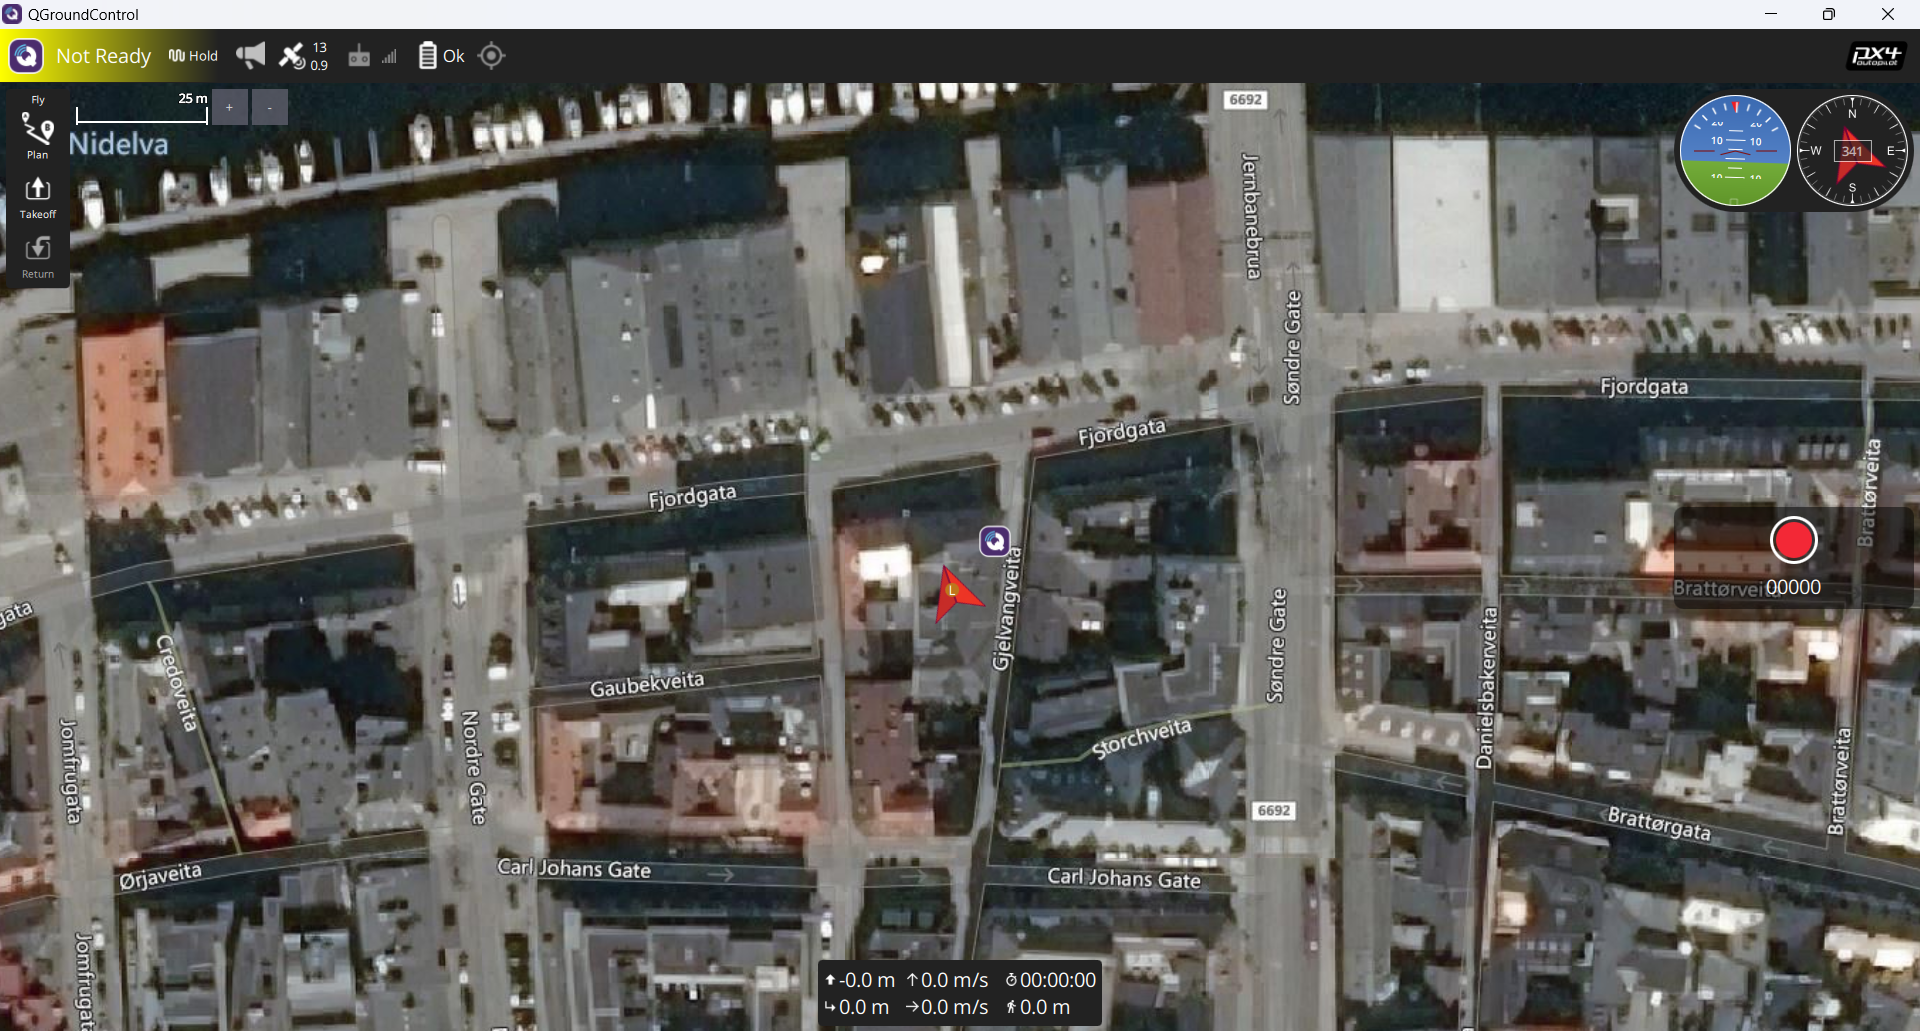
\includegraphics[width=\textwidth,keepaspectratio]{img/qgc-map.png}
  \caption{Main interface for the QGroundControl program.}
  \label{fig:qgc-map}
\end{figure}

\subsubsection{Unreal Engine and AirSim}
\label{subsec:unreal}

Unreal Engine\footnote{\url{https://www.unrealengine.com/en-US}} is a versatile 3D computer graphics tool primarily known for its game development capabilities. Initially introduced in 1998 for creating first-person shooters, the engine has evolved over time and is now widely used in various domains such as film, television, and research. It enables the creation of virtual sets, real-time rendering, computer-generated animation, and the development of virtual environments for architecture and vehicle design. Leveraging its real-time graphic generation capabilities, Unreal Engine serves as a powerful foundation for virtual reality applications. The interface of the engine, as shown in Figure \ref{fig:ue-interface}, provides a user-friendly environment for project development.

\begin{figure}
  \centering
  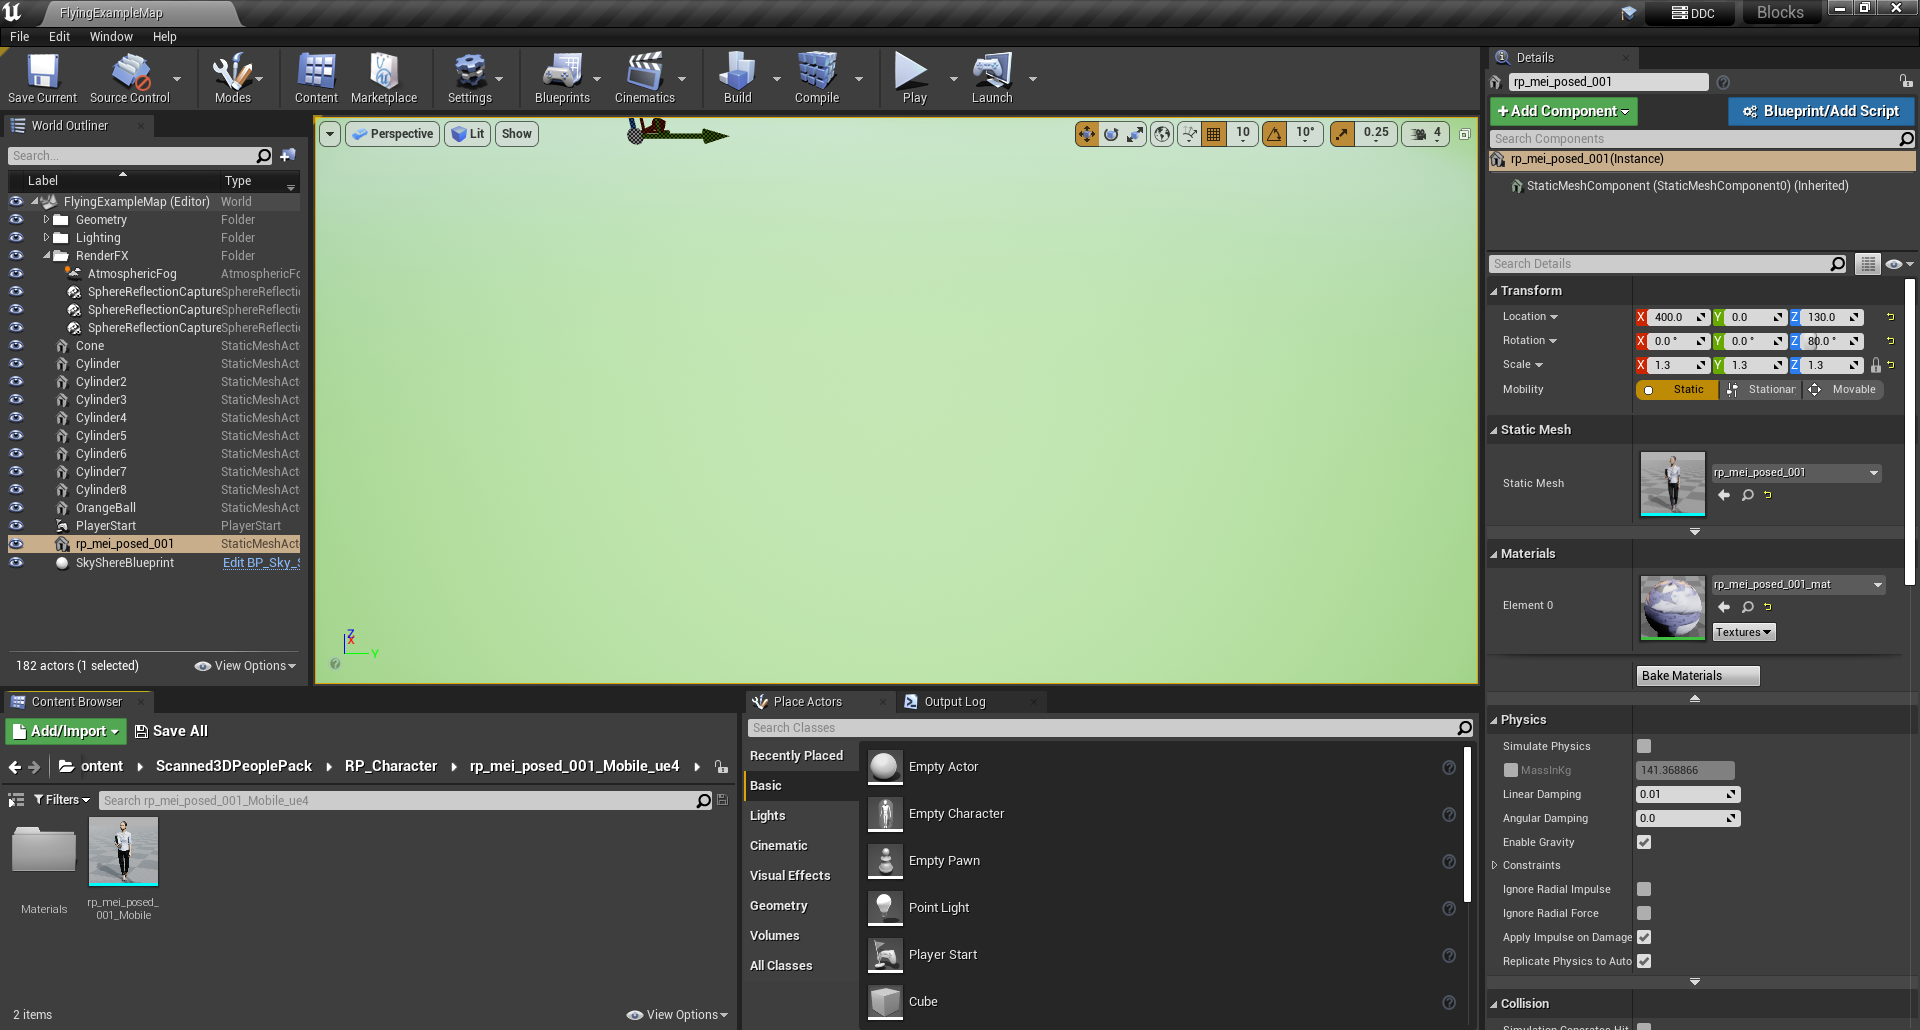
\includegraphics[width=\textwidth,keepaspectratio]{img/ue-interface.png}
  \caption{Project interface for the Unreal Engine.}\label{fig:ue-interface}
\end{figure}


AirSim\footnote{\url{https://microsoft.github.io/AirSim/}}, released by Microsoft in 2017, is an open-source simulator built on Unreal Engine. Designed for drones, cars, and other vehicles, AirSim supports both software-in-the-loop (SITL) and hardware-in-the-loop (HITL) simulations. It seamlessly integrates with popular flight controllers like PX4 and ArduPilot, allowing for realistic simulations that encompass both physical and visual aspects. Built as an Unreal Engine plugin, AirSim can be easily incorporated into existing Unreal environments. The main objective of AirSim is to provide a platform for AI research, facilitating experiments with deep learning, computer vision, and reinforcement learning algorithms for autonomous vehicles. To achieve this, AirSim offers APIs for data retrieval and vehicle control in a platform-independent manner. As of 2023, Microsoft has announced the development of a new simulation platform, Project AirSim, which will replace the original 2017 AirSim. While the original version will remain accessible to the public, it will no longer receive updates.

The combination of Unreal Engine and AirSim provides a robust framework for developing and testing autonomous systems. Researchers and developers can take advantage of the advanced capabilities of Unreal Engine to create visually immersive virtual environments, while AirSim's integration enables realistic simulations and AI experimentation. This integration offers a valuable toolset for exploring and advancing the field of autonomous vehicle technology.

AirSim plays a crucial role in this project by providing a simulated environment for testing and evaluating a vision-based control solution for tracking and following a person. By integrating AirSim into the project, the developed control algorithm can be applied to virtual drones within the simulated environment. This allows for comprehensive testing of the algorithm in various scenarios and conditions, providing valuable insights into its performance and effectiveness. Through this integration, the project benefits from the convenience and flexibility of simulation-based testing, ultimately leading to the development of a robust and reliable control solution for real-world deployment.


\subsubsection{MediaPipe}
\label{subsec:mediapipe}
MediaPipe\footnote{\url{https://google.github.io/mediapipe/}}, developed by Google, is an open-source project that provides customizable machine-learning solutions for live and streaming media. It offers a wide range of capabilities, including real-time perception of human pose, face landmarks, and hand tracking. These features enable the development of various applications, such as fitness and sports analysis, gesture control, sign language recognition, and augmented reality effects.

One of the key advantages of MediaPipe is its cross-platform support, allowing it to be used on Android, iOS, desktop/cloud, web, and IoT devices. It is designed to deliver accelerated processing and fast machine learning inference, even on less advanced hardware. This makes it accessible and applicable to a wide range of devices, ensuring that the developed solutions can be deployed on different platforms without sacrificing performance.
MediaPipe offers a flexible framework specifically tailored for complex perception pipelines, making it well-suited for tasks that require real-time analysis of visual data. 

Its versatility and robustness make it a valuable tool for researchers and developers working on computer vision and machine learning projects, empowering them to create innovative applications that leverage the power of streaming media, like the live feed from a camera onboard a drone.
Given the constraints of the onboard hardware for this project, which may have limited processing capabilities, Mediapipe's ability to perform on smaller devices becomes essential. 


\subsubsection{GitHub}
\label{subsec:github}

GitHub is an online hosting service that utilizes the Git version control system for software development. It serves as a centralized platform for storing code repositories, making it easy to manage and collaborate on projects. With a massive user base and millions of repositories, GitHub has become the leading source code host. 
In this project, both the software code\footnote{\url{https://github.com/l-gonz/tfg-giaa-dronecontrol}} and this report\footnote{\url{https://github.com/l-gonz/tfg-giaa-memoria}} are stored in GitHub. This allows for seamless version control and easy access to the project's codebase. 
Additionally, GitHub allows users to create static websites directly from repositories through GitHub Pages. This feature  serves as an ideal solution for creating a landing or presentation page for the project\footnote{\url{https://l-gonz.github.io/tfg-giaa-dronecontrol/}}. The page contains an overview of the project's goals and implementation details, accompanied by videos showcasing the tests conducted in Chapter \ref{chap:validation}.


\subsubsection{OpenCV}
\label{subsec:opencv}

OpenCV is a widely used open-source library for computer vision, machine learning, and image processing, offering a rich collection of over 2000 algorithms. It provides powerful capabilities for various image-related tasks, such as capturing images or videos from cameras, extracting valuable information from them, and performing image editing operations.

Developed primarily in C++, OpenCV also offers Python wrappers, allowing users to leverage the flexibility and simplicity of Python while benefiting from the optimized performance of the underlying C++ code. OpenCV-Python integrates seamlessly with the Numpy library, which specializes in efficient numerical operations and adopts a MATLAB-like syntax. This integration enables smooth data exchange between OpenCV and other libraries, like Matplotlib, for convenient graph plotting.

In this project, the OpenCV and Numpy libraries play a crucial role in managing image data and facilitating communication with the MediaPipe library. They are utilized to process image information, illustrate detected landmarks, and enable the annotation of images within the DroneVisionControl application's graphical user interface. Additionally, Matplotlib has been employed to generate the graphs presented in Section \ref{sec:test-1-pid}. These libraries collectively contribute to the effective handling and analysis of image-related tasks throughout the project.

\subsection{Hardware}
\subsubsection{Pixhawk 4}
\label{subsec:pixhawk}

The Pixhawk 4 is an advanced autopilot module developed by Holybro\footnote{\url{https://shop.holybro.com/}} in collaboration with the Dronecode Project team. It is designed based on the open hardware design of the Pixhawk-project\footnote{\url{https://pixhawk.org/}} and optimized to run the PX4 flight stack on the NuttX\footnote{\url{https://nuttx.apache.org/}} operating system.

Equipped with an integrated accelerometer, gyroscope, magnetometer, and barometer, the Pixhawk 4 can autonomously control unmanned aerial vehicles using the native capabilities of the PX4 flight stack. These built-in sensors provide essential data for flight control and navigation.
Additionally, the Pixhawk 4 offers a range of connector sockets, depicted in Figure \ref{fig:pixhawk4}. The connectors allow for the expansion of its functionality with external sensors, input/output devices, or a companion computer.
These features, combined with its powerful capabilities, make the Pixhawk 4 an integral component in the project's hardware setup.

\begin{figure}[H]
  \centering
  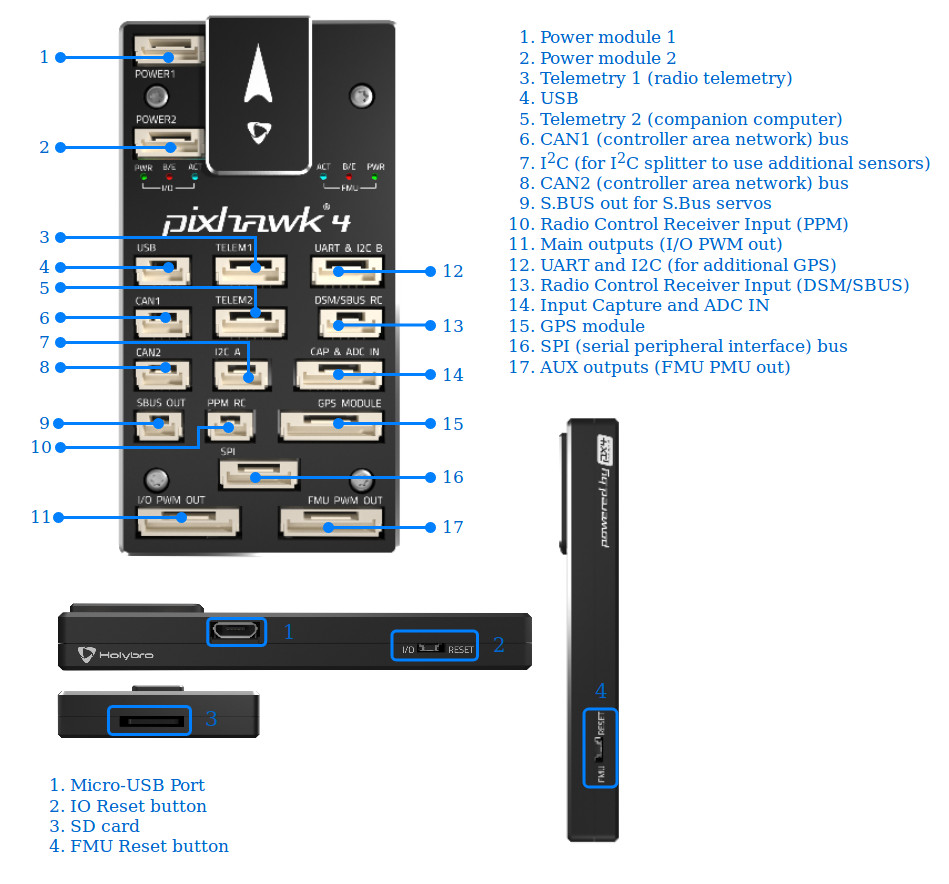
\includegraphics[width=0.6\textwidth,keepaspectratio]{img/pixhawk4.jpg}
  \caption{Side views and connector map for the Pixhawk 4 autopilot module.}
  \source{Adapted from \citetitle{px4-guide} \cite{px4-guide}.}
  \label{fig:pixhawk4}
\end{figure}


\subsubsection{Holybro X500}
\label{subsec:x500}

The Holybro X500\footnote{\url{https://docs.px4.io/main/en/frames_multicopter/holybro_x500_pixhawk4.html}} is a quadcopter specifically designed by Holybro to be compatible with the PX4 autopilot system. It is supplied as a comprehensive development kit that consists of essential components for assembly. These components include a durable carbon-fibre twill frame, the Pixhawk 4 flight controller, a power management board, four motors, a GPS module, an RC receiver, and a telemetry radio. The kit is designed for easy assembly, with a build time of approximately 3 hours and no need for specialized tools. The completed quadcopter is depicted in Figure \ref{fig:x500}, showcasing the final outcome of the assembly process.

\begin{figure}[H]
  \centering
  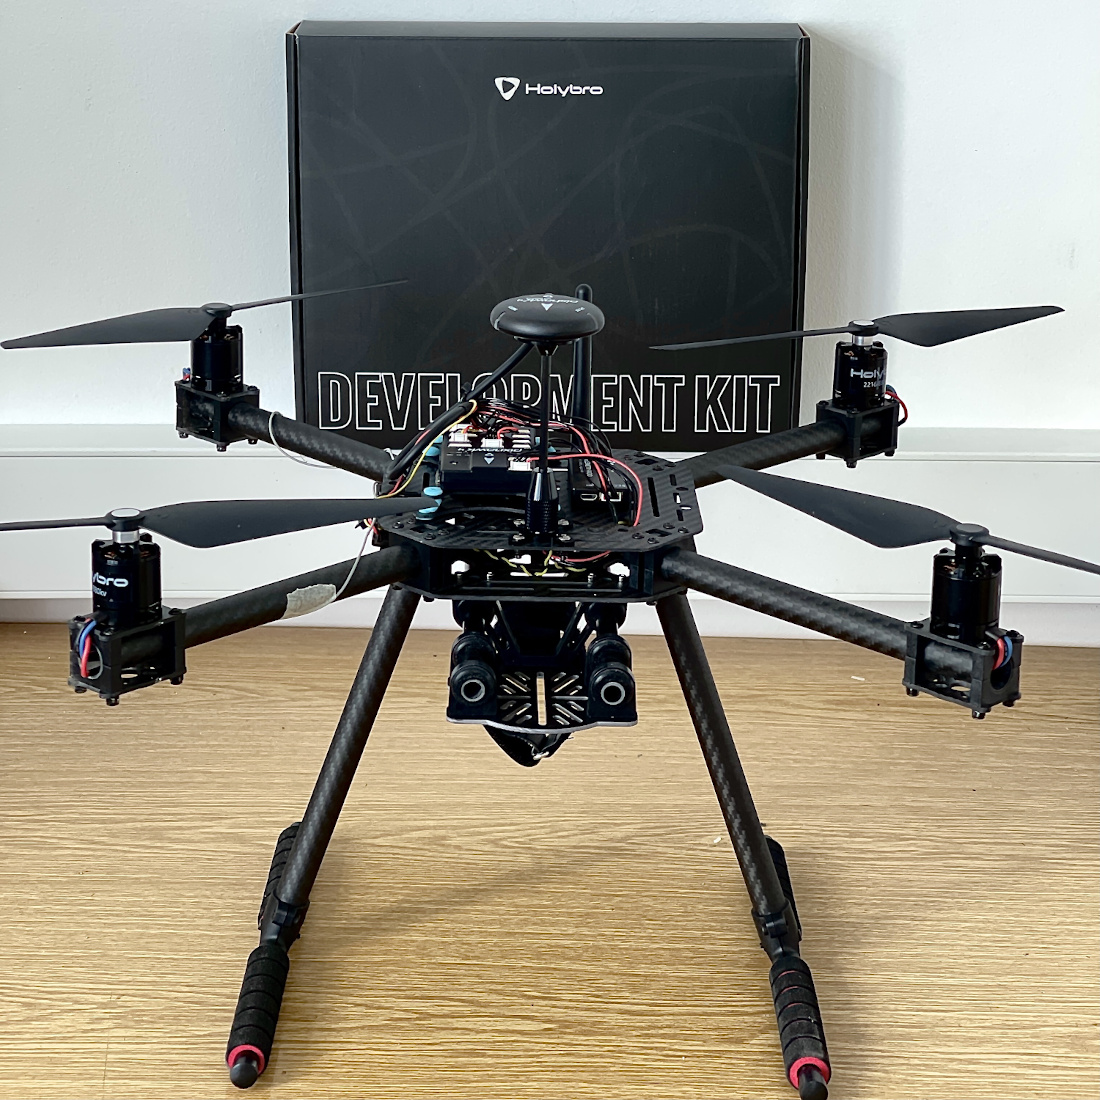
\includegraphics[width=0.5\textwidth,keepaspectratio]{img/X500-assembled.jpg}
  \caption{Fully assembled X500 kit.}
  \source{Adapted from \citetitle{px4-guide} \cite{px4-guide}.}
  \label{fig:x500}
\end{figure}

\subsubsection{Raspberry Pi 4B}
\label{subsec:rpi}

The Raspberry Pi is a series of single-board computers known for their affordability, compact size, and user-friendly design. The Raspberry Pi Model 4B\footnote{\url{https://www.raspberrypi.com/products/raspberry-pi-4-model-b/}}, used in this project, offers improved performance, expanded video output capabilities, and enhanced peripheral connectivity compared to previous models. Despite these advancements, it maintains the same affordable price and compact form factor.

The Raspberry Pi 4B computer comes as a bare circuit board without any additional components like a housing or cooling fan, as shown in Figure \ref{fig:rpi4b}. It features various ports, including USB, HDMI, and Ethernet, as well as built-in Wi-Fi and Bluetooth connectivity. Additionally, it provides a 40-pin GPIO (General Purpose Input/Output) header, allowing direct connection of external devices for expanded functionality.
The Raspberry Pi runs the Raspbian OS, a free operating system based on Debian that is specifically optimized for Raspberry Pi hardware. However, it is also compatible with other Linux distributions, which offers flexibility in software choices.

By leveraging the Raspberry Pi 4B as a companion computer to the Pixhawk 4 board, computationally intensive computer vision tasks are offloaded to a dedicated processor. Thanks to its compact size, it can be integrated onboard the vehicle to facilitate real-time processing of a camera feed from an attached camera. This setup enhances the capabilities of the system by leveraging the Raspberry Pi's processing power for efficient and responsive image analysis during flight operations.

\begin{figure}[H]
  \centering
  \includegraphics[width=0.5\textwidth,keepaspectratio]{img/rpi4b.jpg}
  \caption{Raspberry Pi 4 Model B}
  \source{Wikimedia Commons \cite{rpi4-side}.}
  \label{fig:rpi4b}
\end{figure}

\clearpage

% DISEÑO E IMPLEMENTACIÓN %
\chapter{Design and implementation}
\label{chap:design}
\todo[inline]{Summary Chapter 3}

\section{Simulation and development environment}
\label{sec:devenv}
Simulation plays a crucial role in developing vision-based control solutions for UAVs. It offers a safe and cost-effective environment to explore and refine algorithms, test new capabilities, and evaluate system performance without the risks associated with real-world flights. 
In this context, simulation refers to creating a computer-generated virtual environment that mimics a UAV's real-world conditions and interactions. In this simulation, various aspects of the UAV system, including the flight dynamics, sensor inputs, and environmental factors, are replicated and simulated in a software-based environment.

This section explores how simulation is implemented in the PX4 platform and the development environment built around it for this project to develop the hand-gesture and person-following control solutions mentioned before.
The three key simulation components are examined individually: the simulated flight stack, the simulation engine or simulator, and the companion computer for offboard control. 
The two available simulation modes, \acrfull{sitl} and \acrfull{hitl}, are introduced for the flight stack. In contrast, the simulation engine encompasses modelling physical world components and the physics and rendering engines. 
The communication between the simulator, flight controller firmware, and companion computer is also described. 
Lastly, the development environment is discussed, covering network configurations and using Unreal Engine and AirSim as the simulation engine for this project.

\subsection{SITL and HITL simulation}

The PX4 platform is a flexible and powerful open-source flight control software stack widely used for developing for UAVs. The platform’s flight stack is the core software responsible for controlling the UAV's behaviour and executing flight commands. It offers comprehensive support for simulation, providing developers with a robust environment to test and refine their control solutions.

There are two main simulation modes for the flight stack: \acrfull{sitl} and \acrfull{hitl}. SITL simulation enables the flight stack to run on a non-dedicated computer, simulating the flight controller’s operating system and allowing for rapid development and testing. On the other hand, HITL simulation executes the simulation firmware on an actual flight controller board, providing a more realistic testing environment. In this mode, the flight stack runs in its native environment while the sensor data and other external inputs are simulated.

Both simulation modes in the PX4 platform offer distinct advantages and are suited for different stages of development. SITL simulation allows developers to iterate quickly, reducing development time and providing immediate visual feedback on the computer screen. This mode is particularly beneficial during algorithm exploration and refinement. HITL simulation, on the other hand, offers increased realism by testing on an actual flight controller board. It allows developers to evaluate their vision-based control solutions in a more accurate representation of the real-world environment. This mode is especially valuable when fine-tuning algorithms and assessing system performance.

In the simulation context, two inextricable components exist: the simulated flight stack (running on SITL or HITL mode) and the simulation engine or simulator. The flight stack interacts with the simulator through a feedback loop, enabling a seamless exchange of information between the two components, as shown in Figure \ref{fig:simulator-loop}.
The feedback loop begins with the simulator generating sensor inputs, such as acceleration measurements or GPS data, based on its internal representation of the simulated world. These sensor inputs are then transmitted to the flight stack.
Upon receiving the sensor inputs, the flight stack processes this information and generates response actuator controls, including motor commands or control signals for various UAV components, which are then sent back to the simulator. Finally, the simulator utilises these actuator controls to update the virtual vehicle's position, velocity, and attitude within the simulated world, thereby simulating the UAV's response to the flight stack's commands. 

This interaction between the flight stack and the simulator within the feedback loop allows for a dynamic and synchronised simulation experience, mimicking the behaviour of a real-world UAV by providing realistic sensor inputs and simulating the corresponding actuator responses.
All communication between the flight stack and the simulator is implemented using the MAVLink messaging protocol and the UDP transport protocol. MAVLink messages serve as a standardised format for transmission, allowing the seamless exchange of information between the two components.

\begin{figure}
  \centering
  
\includegraphics[width=\textwidth,keepaspectratio]{img/px4-simulator-loop.png}
  \caption{Feedback loop during the PX4 simulation.}
  \source{Adapted from \citetitle{px4-guide} \cite{px4-guide}.}
  \label{fig:simulator-loop}
\end{figure}

\subsection{Simulator}

%\texttt{airlib}\footnote{\url{https://pypi.org/project/airsim/}}

\begin{figure}
  \centering
  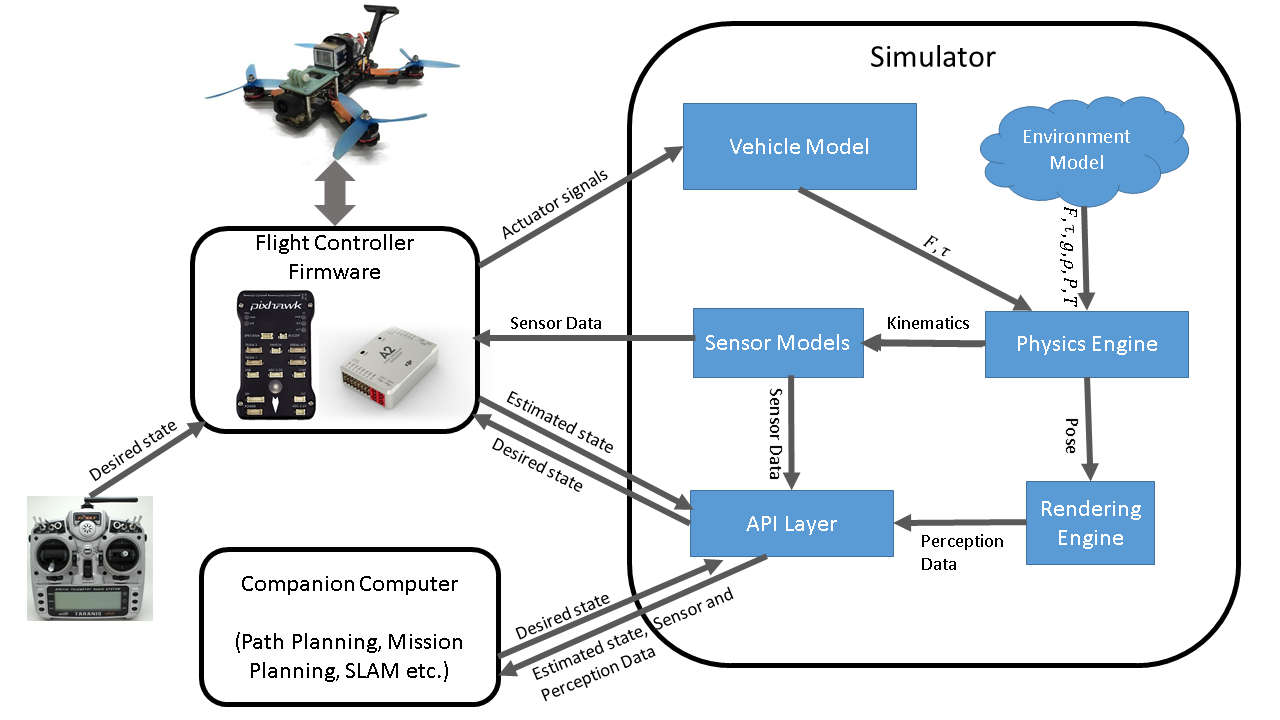
\includegraphics[width=\textwidth,keepaspectratio]{img/airsim-overview.png}
  \caption{High-level overview of how different components of a simulator interact with the flight stack.}
  \source{Adapted from \citetitle{airsim-paper} \cite{airsim-paper}.}
  \label{fig:airsim-overview}
\end{figure}

The simulator plays a crucial role in development by providing visual feedback on the vehicle’s reactions to the control software.
Inside the simulator, a group of components that model real-world elements work together to make up the complete engine.
Figure \ref{fig:airsim-overview} expands upon the diagram in Figure \ref{fig:simulator-loop} to show the high-level overview of how each of these components interacts with each other and with the flight controller firmware (flight stack).

The environment model represents the virtual world where the simulation occurs, providing the simulated surroundings and obstacles for the UAV. It can include terrain and weather conditions that affect flight dynamics, like wind or variable temperatures, which are sent to the physics engine. 
The vehicle model represents the UAV's physical characteristics, such as its mass, size, aerodynamics, and propulsion system, which are simulated to generate forces and moments based on actuator signals.
The sensor model simulates the behaviour and outputs of cameras, lidars, and \acrshort{imu}s, providing realistic sensor data to the flight stack.
The physics engine governs the laws of physics within the simulation, calculating forces, torques, collisions, and other physical interactions to ensure that the vehicle and its environment interact realistically.
The rendering engine is responsible for rendering the visual aspects of the simulation, allowing for realistic graphics and visualisation.
The final component of the simulator is the \acrshort{api} layer. It serves as a communication interface between the simulator and the flight stack, facilitating the exchange of data and control commands through the MAVLink protocol. This API can also connect the simulator to an external companion computer to use the sensor and state data provided. 

In this context, the companion computer is an additional computational device that works together with the flight controller firmware and the simulator. It aims to offload specific tasks and computations from the flight controller, enabling more complex algorithms, higher-level control, and real-time data processing. The companion computer allows implementing vision-based control solutions, as it can handle intensive image processing and machine learning. It facilitates the integration of advanced perception, planning, and decision-making capabilities, enhancing the UAV's autonomy and enabling more sophisticated behaviours in simulated environments.
The communication between the companion computer and the simulation system can be established by the simulator’s own API layer, as shown in Figure \ref{fig:airsim-overview}, or through any dedicated API that can interact with the flight stack through MAVLink messages.
An example of the latter case would be the MAVSDK API mentioned in Section \ref{subsec:mavlink}.
This project will use this method to separate the communication between the flight stack and the companion computer from the simulator.
The separation allows for a more seamless transition into flight tests, where the real world replaces the simulator component.

There are many options for simulators supported by PX4.
The simpler of these is jMAVSim, which can be installed along with the PX4 SITL simulation on a Linux system. It provides a lightweight simulation environment for PX4, allowing for basic testing and evaluation of flight control algorithms. While it may lack some advanced features, jMAVSim is a convenient option for checking that the simulated flight stack has been configured correctly during initial development iterations.
A second option for running on Linux is Gazebo. Gazebo is a powerful simulator widely used in robotics and compatible with PX4. It offers more advanced capabilities, such as obstacle avoidance and support for the Robot Operating System (ROS). It provides a realistic physics engine for simulating UAV dynamics and environments and enables the integration of complex sensor models, making it suitable for testing perception and navigation algorithms. However, it is more limited in graphics, which becomes critical when testing control solutions driven by computer vision.

The last option considered to fulfil the requirements of the project is AirSim. This simulator is built as a plugin for the popular Unreal Engine, designed for game development. Unlike jMAVSim and Gazebo, AirSim runs on Windows and leverages the capabilities of a game engine. It provides visually and physically realistic simulations, offering advanced graphics and rendering capabilities. AirSim is particularly advantageous for testing computer vision features as it offers easy access to thousands of visual packages through its asset library. Its integration with Unreal Engine enables the creation of complex and immersive simulated environments. These features make it especially suited for developing vision-based control solutions, making it the best choice for this project.


\subsection{Development environment}

This section discussed the configuration adopted in this project to establish connections between the developed control software, the selected AirSim simulator, and the flight stack. It encompasses both SITL and HITL simulation modes, which allow testing the implementation of the \texttt{drone-vision-control} application within a controlled environment. While the application is designed to leverage the dedicated processing power of a companion computer in real-world scenarios, during simulation, it will primarily operate on the same computer hosting the simulation engine to minimise physical connections between multiple machines.

\subsubsection{SITL configuration}

\begin{figure}
  \centering
  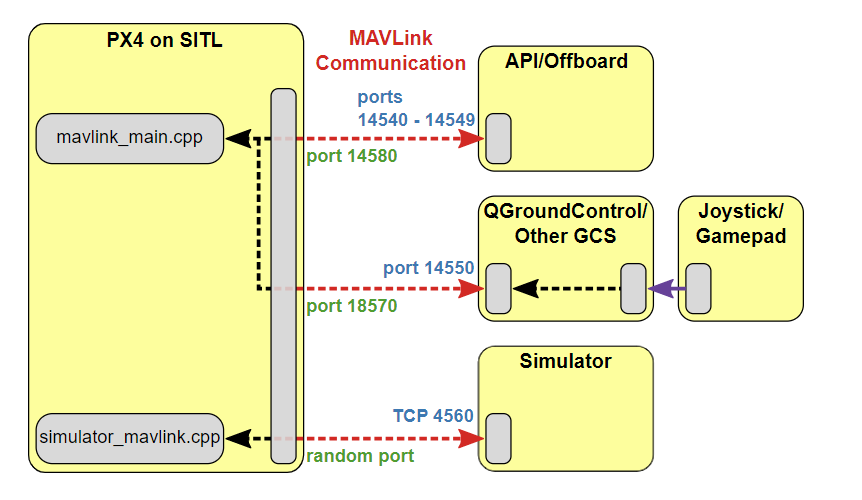
\includegraphics[width=\textwidth,keepaspectratio]{img/px4-ports.png}
  \caption{Network diagram between the components interconnecting during software-in-the-loop simulation.}
  \source{Adapted from \citetitle{px4-guide} \cite{px4-guide}.}
  \label{fig:px4-ports}
\end{figure}

The PX4 platform has an established network configuration for SITL simulation, shown in Figure \ref{fig:px4-ports}. The figure’s left side shows the two programs that manage MAVLink servers for communicating with components outside the flight stack. The first is the main MAVLink manager, inherent to the PX4 system. It expects connections from offboard control sources, such as a companion computer using an offboard API (MAVSDK) or a ground control station like QGroundControl (\ref{subsec:qgc}). These connections are established using the \acrshort{udp} protocol on the port range 14540-14550. By default, port 14550 is reserved for a ground station but can be used by any other offboard application if \acrshort{qgc} is not required.
The second server runs exclusively during simulations and connects to the simulator program instead through a \acrshort{tcp} connection, as it requires higher reliability than the offboard connections.

In this project, the simulator will run on a Windows system, as that is the native environment of the AirSim simulator. The SITL simulation, however, runs best on Linux. To execute both software components simultaneously on a single machine, the \acrfull{wsl} \cite{wsl-learn} will be utilised. WSL allows for the execution of a Linux distribution, such as Ubuntu, directly within the Windows operating system, providing a convenient environment for running PX4 SITL alongside AirSim without the need for dual-booting or virtual machines. This configuration ensures that the connections are limited to the machine’s internal network, as WSL handles the task of establishing network connectivity between the Windows and Linux environments. It achieves this by setting up a virtual Ethernet bridge and ensuring network traffic is routed appropriately.
The complete steps needed to configure the PX4 WSL system are detailed in Appendix \ref{app:install-dev-env}.


\begin{figure}
  \centering
  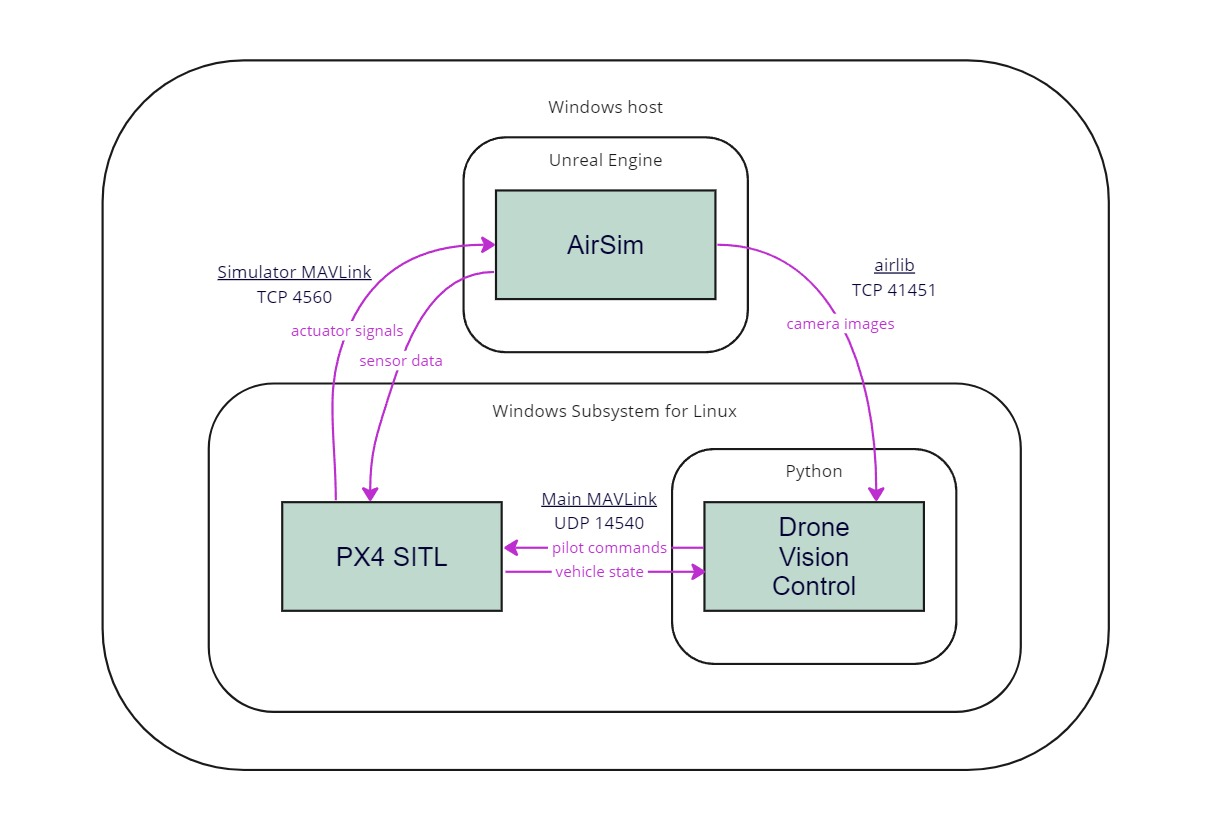
\includegraphics[width=0.8\textwidth,keepaspectratio]{img/sitl-connections.jpg}
  \caption{Connection diagram of how the three systems interact with each other during SITL simulation.}
  \label{fig:sitl-connections}
\end{figure}
\todo[inline]{Edit: rename dronecontrol, change UDP port, virtual bridge, add airlib/mavsdk/simulator-mavlink to arrows, AirSim - PX4 should be bidirectional arrow}

The whole set of connections necessary between the three individual components at the transport layer level during SITL simulation is shown in Figure \ref{fig:sitl-connections}.
The AirSim simulator runs as part of the Unreal Engine application directly on the host Windows system. It connects to the other two components running inside the virtualised Linux subsystem through the established bridge. AirSim and the PX4 flight stack exchange information through the TCP connection to the secondary MAVLink server, as shown in Figure \ref{fig:px4-ports}.

The communication between AirSim and the \texttt{drone-vision-control} application is facilitated through the API layer depicted in Figure \ref{fig:airsim-overview}, which can connect the simulator with a companion computer or other system running additional code. This connection is established using the \texttt{airlib} library developed for Python by the creators of AirSim, which allows easy access to the AirSim API. In this project, the connection between AirSim and the application through \texttt{airlib} transmits only perception data, specifically camera images of the simulated world. 
For the transmission of other data, such as the current vehicle state from the simulator to the application and the desired state from the application to the simulator, a direct connection between the flight stack and the application is used instead, as this is the only link that can be maintained in a real-world scenario. This direct link is established through the main MAVLink instance of the flight stack, as illustrated in Figure \ref{fig:px4-ports}.

Given that the application is developed in Python, a versatile programming language compatible with multiple platforms, it can be run either on the central Windows system or within the virtualised Linux subsystem. However, running the application on Linux is more advantageous to avoid the need for the MAVLink server to broadcast to the Windows system.



\subsubsection{HITL configuration}

\begin{figure}
  \centering
  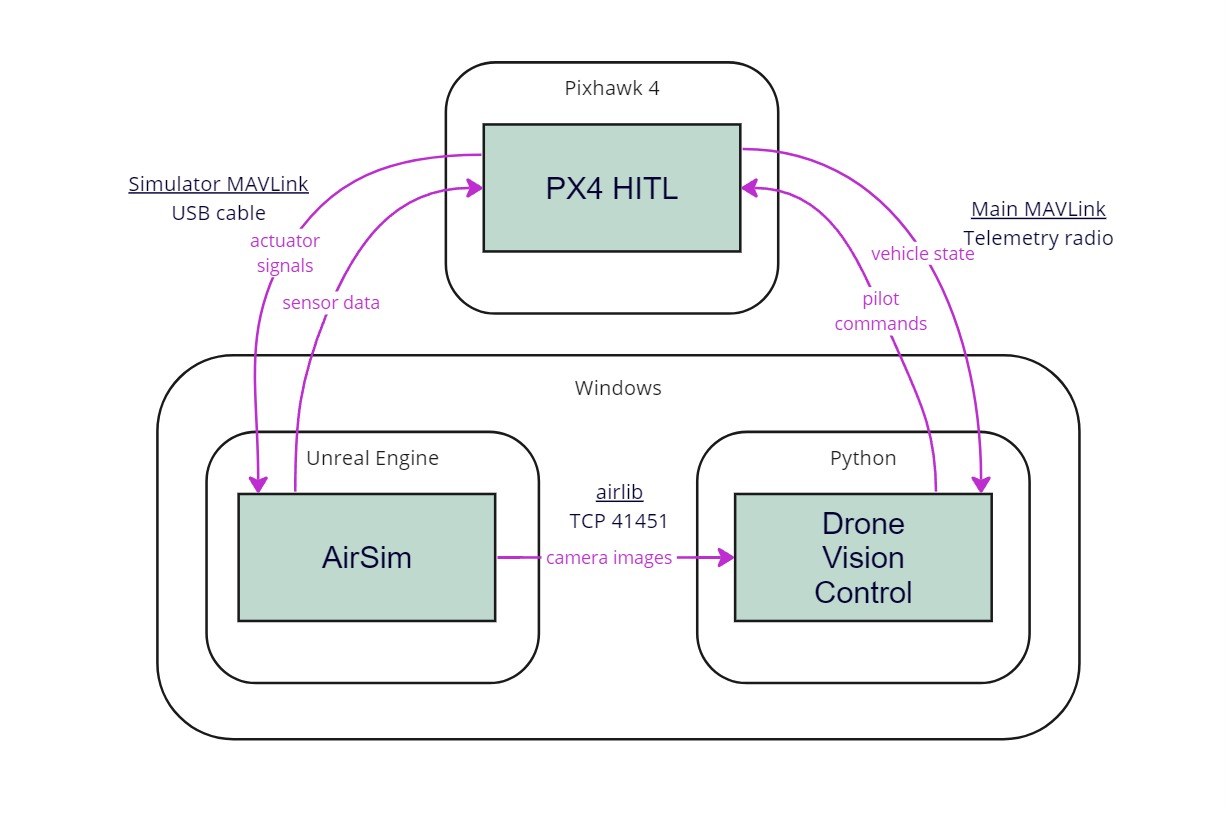
\includegraphics[width=0.8\textwidth,keepaspectratio]{img/hitl-connections.jpg}
  \caption{Connection diagram of how the three systems interact with each other during HITL simulation.}\label{fig:hitl-connections}
\end{figure}
\todo[inline]{Rename app}

Transitioning from SITL to HITL simulation involves shifting from the WSL environment to a physical flight board, specifically a Pixhawk flight controller, to run the flight stack firmware. In HITL simulation, the flight board's motors and actuators are blocked, but the internal software functions fully. The Python execution will also be moved from the Linux subsystem to the Windows host. This transition simplifies the testing process by eliminating the need for additional configurations to establish communication between the flight controller and the internal WSL network, which is isolated from external machines by default.

As the flight stack now runs on separate hardware, it becomes necessary to establish a physical connection between the testing computer and the flight controller for each desired MAVLink channel. This connection can be set up using the debug micro-USB port on the flight controller or any available telemetry ports, which allow serial connections to external systems. These connections can be established, for example, using a serial-to-USB converter or through a pair of telemetry radios. The simulator and the Python application can communicate independently with the flight controller by using several of these options simultaneously.

Figure \ref{fig:hitl-connections} illustrates the chosen connections for executing tests in HITL mode. The Windows machine hosts both AirSim in Unreal Engine and the Python interpreter running the developed application, which keep their communication through the \texttt{airlib} library. In this case, there is no need for the virtual bridge network, and the TCP connection is established through the \texttt{loopback} network. The PX4 flight controller is connected to the simulator via a USB to micro-USB cable, configured with a baud rate of 115200. It is also connected to the Python program through a telemetry radio operating at a baud rate of 57600. Both connections on the Windows computer side are attached to USB ports. These ports are accessible via their respective COM addresses, which must be specified in the configuration for AirSim and MAVSDK.


\subsubsection{AirSim environment}

Microsoft develops the AirSim simulator as a plugin in the computer graphics and game development program Unreal Engine.
It implements sensor, vehicle and environment models appropriate for flight simulation while taking advantage of the physics and rendering engines integrated into Unreal.
In the engine, projects comprise one or more environments where components like 3D models, cameras, and lighting can be added. 
The source code for the AirSim project includes a basic Unreal environment with all the minimum components already configured that can be used to test the implementation or as a starting point for more complex environments. It contains several 3D shapes like blocks and spheres and a simple quadcopter to act as the simulated vehicle.
Creating custom Unreal environments and running AirSim inside them is also possible by manually adding the built plugin and a vehicle to an existing project.

The environment used in this project for testing the \texttt{drone-vison-control} application is derived from the base AirSim environment and can be found on the project’s repository\footnote{\url{https://github.com/l-gonz/tfg-giaa-dronecontrol/tree/main/data}}. It contains the default quadcopter vehicle, which includes several virtual cameras that allow retrieving images from the vehicle’s point of view in the simulated world. 
The main addition to the environment is the 3D model of a human figure, to be used for testing the human detection and tracking mechanisms in the computer vision solution. This model is part of a free asset library of human models made by Renderpeople \cite{render-people} obtained from the Unreal Marketplace.
Some minor modifications have also been made to the background shapes and colours to provide better contrast for the camera.
Figure \ref{fig:unreal-env} shows an image of the testing environment as seen from the Unreal viewport in Edit mode.

\todo[inline]{Add here if any additional changes to AirSim environment}


\begin{figure}
  \centering
  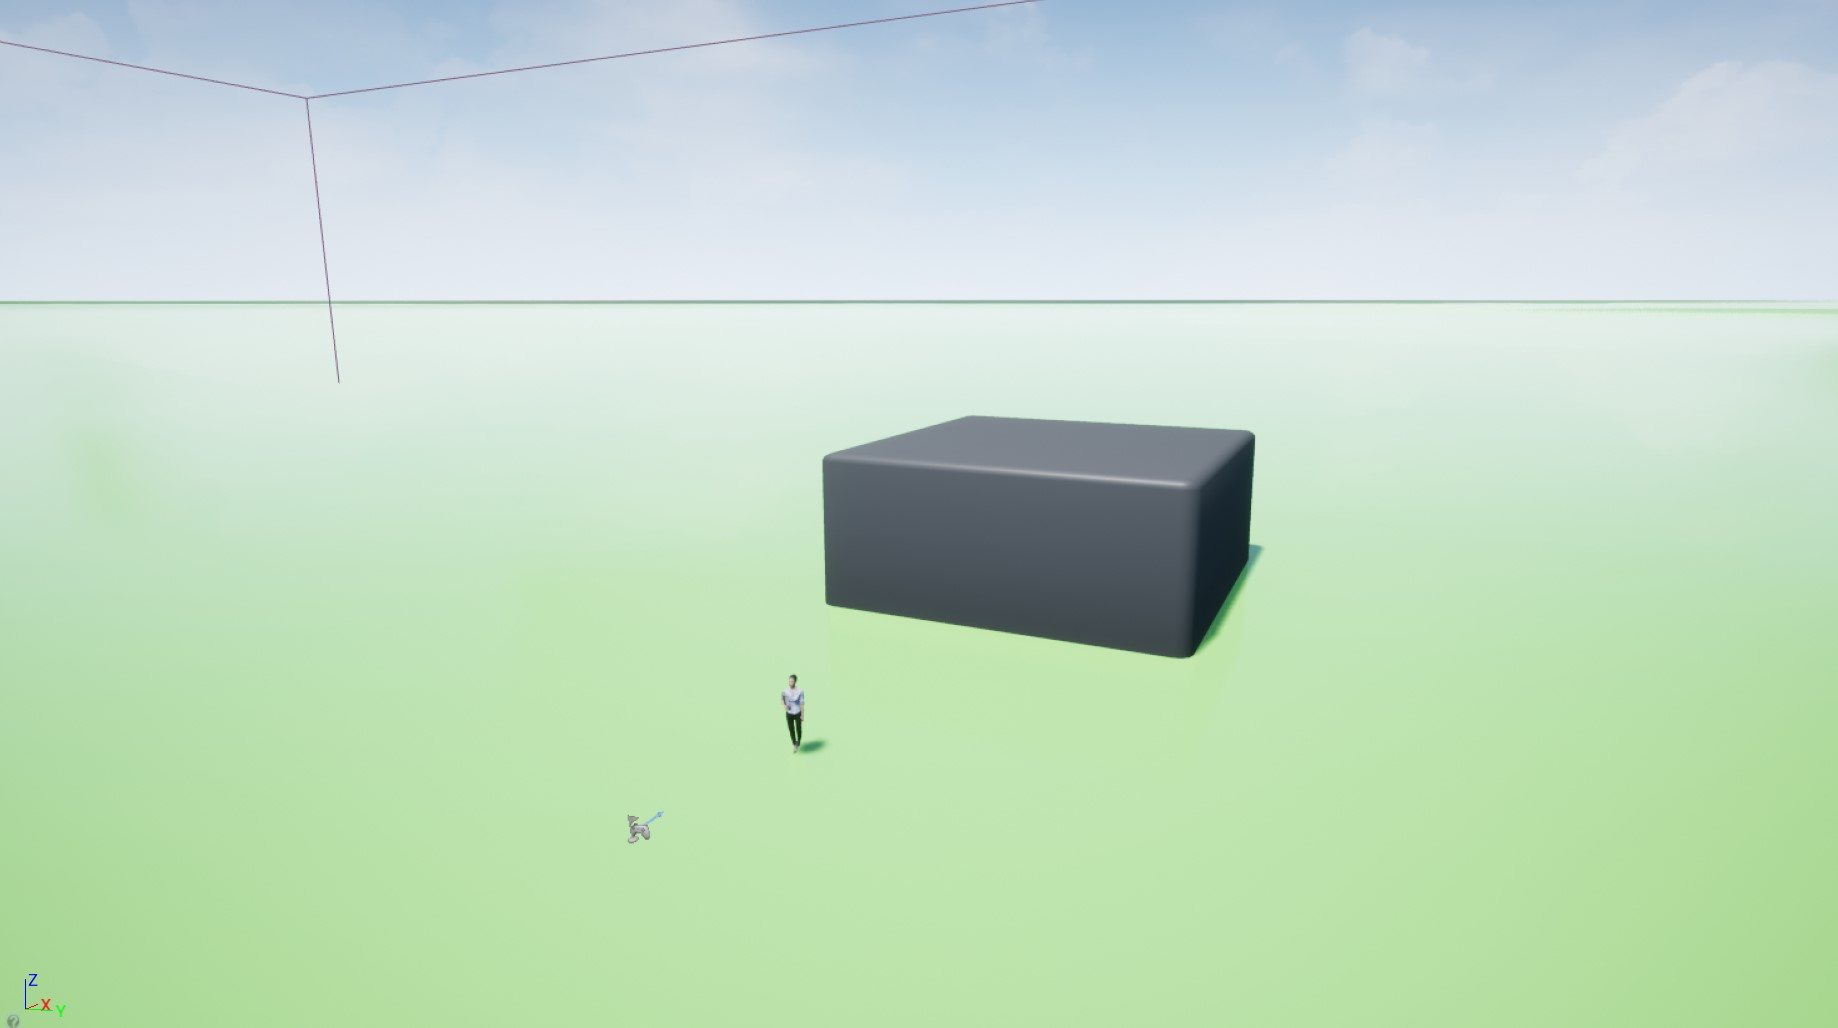
\includegraphics[width=\textwidth,keepaspectratio]{img/unreal-env.jpg}
  \caption{Screenshot from the Unreal Engine environment used for testing the computer vision solutions.}
  \label{fig:unreal-env}
\end{figure}


AirSim is compatible with both SITL and HITL simulation modes and several other flight stacks apart from PX4, including AirSim’s own internal SimpleFlight flight stack, which is used by default. 
The plugin must therefore be configured for this project to work with the desired simulation setup (PX4 + WSL + Airsim).
This process is explained in the AirSim documentation \cite{build-airsim} by its developers and in Appendix \ref{app:install-dev-env} for more project-specific details.
Appendix \ref{app:airsim-config} contains the complete settings file used in this project for configuring PX4 with either simulation mode in AirSim, including the parameters that must be individualised for each system.
\todo[inline]{Move to Appendix A.3}
%, where the ”LocalHostIp” needs to be exchanged with the IP of the Windows host in the local vEthernet (WSL) network to be able to connect between the simulator in Windows and the flight controller inside WSL. For HITL, the ”UseSerial” setting should be set to true in the AirSim configuration, and the Pixhawk board should be connected to a USB port in the computer. 


To start the simulation in AirSim, the following steps must be followed:
\begin{enumerate}
 \item Attach physical flight controller in HITL mode to simulation computer (HITL only).
 \item Start play mode in Unreal.
 \item Build and start simulated flight stack in WSL (SITL only).
 \item Start companion applications, if any (e.g. \texttt{drone-vison-control}, QGroundControl).
\end{enumerate}

To build and start the PX4 SITL flight stack for AirSim, a small script can be found in the project source code\footnote{\url{https://github.com/l-gonz/tfg-giaa-dronecontrol/blob/main/simulator.sh}} that will automatically attach to a running AirSim instance if it is executed with the \texttt{-{}-airsim} option.
To be able to use the physical flight board for HITL simulation, this mode needs to be enabled from the QGroundControl safety configuration.
Once the simulation has started, there is no noticeable change between the simulated flight controller in WSL (SITL mode) and the one running in the physical board (HITL mode).

\section{System architecture}
\label{sec:sysarch}

This section describes the architecture of the interaction between the flight controller and the DroneVisionControl application. It outlines the key components of the system along with their connections, discussing two possible configurations: offboard, where the companion computer acts as a ground station, and onboard, where the companion computer and camera are onboard the vehicle. The following sections explore the details of each configuration.

\subsection{Top-level components}

\begin{figure}
  \centering
  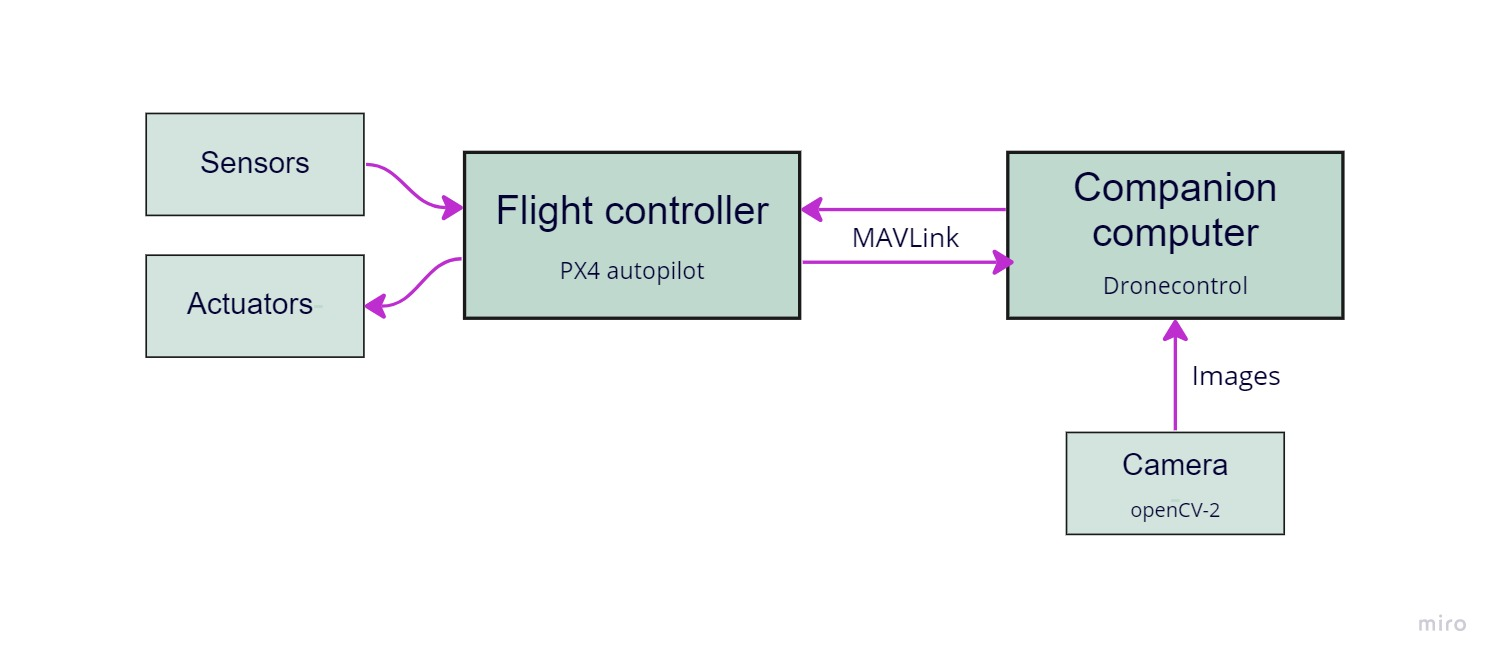
\includegraphics[width=0.9\textwidth,keepaspectratio]{img/sys-arch-diagram.jpg}
  \caption{Top-level diagram of the hardware/software interactions}
  \label{fig:toplevel}
\end{figure}


The DroneVisionControl application aims to direct the movement of a UAV by analyzing images captured by a camera. Since the processing power needed to analyse the images exceeds the capabilities of the autopilot flight controller, an additional companion computer is necessary. This companion computer will control the camera and utilise machine learning algorithms to extract useful features from the images and convert them into movement directives for the vehicle.

Figure \ref{fig:toplevel} illustrates a top-level diagram depicting the key components of the system. The main elements include the flight controller, running the PX4 autopilot firmware, the companion computer hosting the developed application, and the camera responsible for image capture.  The camera connects to the companion computer using a USB cable plugged into any available port. The flight controller establishes the communication with the companion computer via the MAVLink protocol described in section \ref{subsec:mavlink}, either through telemetry radios or a direct wire connection. The choice of connection type depends on the desired setup of the system.

In the simplest configuration, the companion computer can function as a ground station, directing the vehicle's movement from the ground while the flight controller remains onboard. This configuration is possible when the camera doesn't need to move with the vehicle. In this scenario, wireless communication becomes critical, so it will be established utilizing a pair of telemetry radios. Section \ref{subsec:offboard} provides a comprehensive guide for this configuration.

Alternatively, when the camera needs to move with the vehicle to capture images from its perspective, the companion computer and camera are placed onboard the vehicle alongside the flight controller. In this case, a direct wired connection between the two is the most suitable option, offering a faster and more stable link. Details of this configuration are provided in section \ref{subsec:onboard}.

\subsubsection{The flight controller}

The flight controller or autopilot is a circuit board equipped with sensors, and optimized for running the flight stack.
The autopilot used in this project is the Pixhawk 4, designed by Holybro for the PX4 firmware.
This board depends on a specific set of hardware components to function properly.
These components include sensors, which collect environment data for processing, and actuators, which transform the output signals from the controller into movement.

To determine the vehicle's state for stabilization and autonomous control, PX4 relies on sensors such as gyroscopes, accelerometers, magnetometers (compasses), and barometers.
These are the sensors that are typically included already integrated with the autopilot's board.
Additionally, a GPS or other positioning system is required to enable fully automatic flight modes and assisted features like altitude stabilization or mission planning.

PX4 utilises outputs to control motor speed, flight surfaces (e.g., ailerons and flaps), camera triggers, parachutes, grippers, and other payloads. Brushless motors, controlled by Electronic Speed Controllers (ESCs) connected to the flight controller, rotate the propellers in most PX4 drones. These drones typically employ Lithium-Polymer (LiPo) batteries, which are connected to the system using a Power Module or Power Management Board, providing separate power for the flight controller and ESCs. 

For manual control of the vehicle, a \acrfull{rc} system is employed, consisting of a remote control unit that communicates stick and control positions to a receiver on the vehicle. Advanced RC systems can also receive telemetry information from the autopilot, providing feedback to the operator. Telemetry radios offer an alternative means of communication with the autopilot, establishing a wireless MAVLink connection between a ground control station and a PX4-powered vehicle. This enables real-time parameter tuning, flight mode commands, telemetry inspection, and on-the-fly mission changes.

In an actual UAV, the PX4 software runs on dedicated hardware like the Pixhawk 4 mentioned. This hardware includes all the essential sensors for flight as well as interfaces to connect additional actuators and I/O systems (RC, telemetry radio). 
However, on a simulated environment like the one described in section \ref{sec:devenv}, all the hardware components of the sensors and actuators are simulated on the same computer running the flight stack.

\subsubsection{DroneVisionControl and the companion computer}

The DroneVisionControl application that runs on the companion computer utilizes the Python programming language\footnote{\url{https://www.python.org/}}. Python offers several advantages for projects of this nature, including its high-level, easy-to-use syntax, which results in a more concise code base compared to other languages. Other benefits include Python's versatility and support for object-oriented programming. Moreover, Python has a vast ecosystem of external libraries accessible through its official package manager called \texttt{pip}. This package index\footnote{\url{https://pypi.org/}} contains thousands of well-tested utilities, including many designed for machine learning and image processing. Additionally, Python versions of all the necessary libraries for interacting with PX4 via the MAVLink protocol, for object detection and tracking, and for simulation (MavSDK, OpenCV, AirSim, Mediapipe) are available. Being an interpreted language, Python can run seamlessly on any system with Python installed, eliminating the need to compile separate binaries to run in different operating systems.

The following sections will provide an in-depth exploration of the differences between the two configurations mentioned earlier for offboard and onboard companion computers.

\subsection{Offboard computer configuration}
\label{subsec:offboard}

\begin{figure}
  \centering
  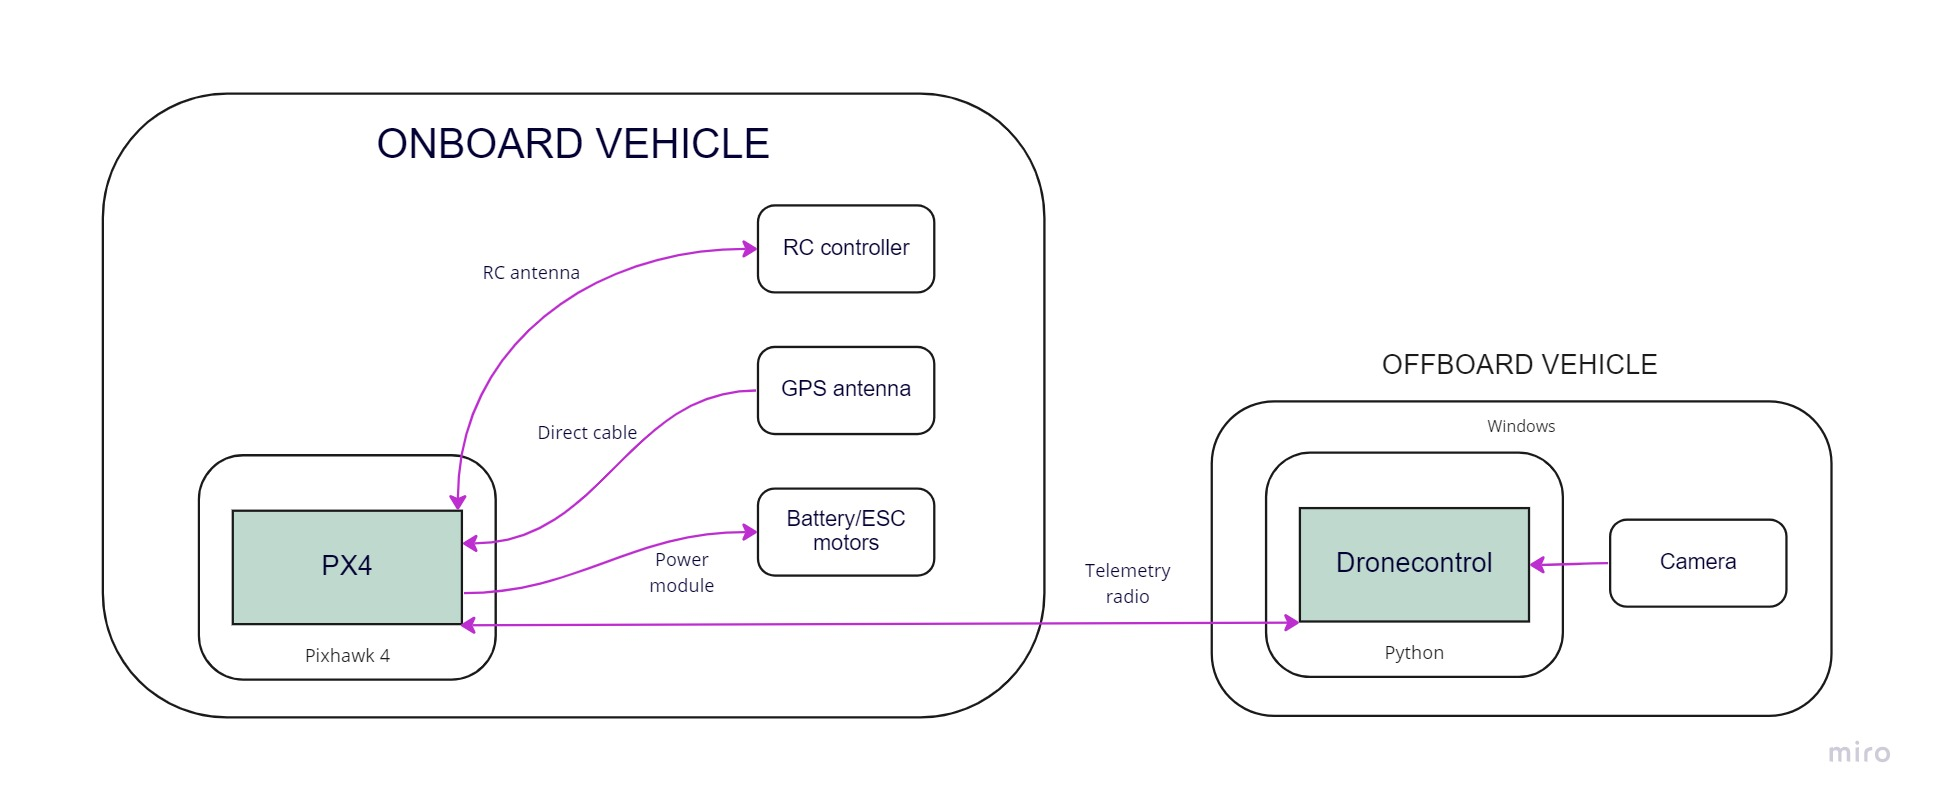
\includegraphics[width=\textwidth,keepaspectratio]{img/offboard-diagram.jpg}
  \caption{Offboard configuration connections}
  \label{fig:offboard-config}
\end{figure}

The offboard configuration allows the flight controller to communicate and receive orders from a companion computer that is not physically connected to its hardware, so the latter can remain on the ground while the vehicle flies.
This configuration offers several advantages, including a simplified setup without concerns about hardware interactions and power supply to the companion computer during flight. It also allows for the use of a more powerful computer for image processing without adding weight to the vehicle. However, the camera remains connected to the ground computer, limiting the system's real-world applications as the images are not captured from the drone's perspective during flight. While other configurations involving direct camera-to-flight controller connection and wireless transmission of images for offboard processing are feasible, they are beyond the scope of this project.

In this configuration, the wireless link is established through a pair of telemetry radios.
These radios connect to a telemetry port on the flight controller and a USB port on the companion computer. 
Since the Pixhawk 4 is configured by default to use its \texttt{TELEM1} port for this purpose, no additional configuration is needed when using that port.
Applications like the QGRoundControl ground station software automatically detect a telemetry radio inserted into any USB port on the host computer and establish the connection to the flight controller.
Additionally, software using the MavSDK library can establish a connection by specifying the USB serial port address and the baudrate of the link, usually something similar to \texttt{/dev/ttyUSB0:57600} on Linux and \texttt{COM1:57600} on Windows.

The radio used for the physical tests in this project is the Holybro SiK Telemetry Radio.
It is a small, light and inexpensive open-source radio platform that typically allows ranges of more than 300 meters "out of the box" (the range can be extended to several kilometres with a patch antenna on the ground).
The radios are offered as 915Mhz (Europe) or 433Mhz (US), so they can be used in different regions and comply with the regulations for frequency, hopping channels and power levels.
They offer 2-way full-duplex communication through an adaptive TDM UART interface, and their antenna allows for an adjustable 100-mW-maximum output power and -117 dBm receive sensitivity.
The link is established by default with a baudrate (max bits per second on a serial channel) of 57600, and it can provide air data rates of up to 250 kbps.

The project utilizes the Holybro SiK Telemetry Radio\footnote{\url{http://www.holybro.com/product/transceiver-telemetry-radio-v3/}} for physical tests. These radios are small, lightweight, and cost-effective, offering a range of more than 300 meters out of the box (which can be extended with a patch antenna). They operate at either 915MHz (Europe) or 433MHz (US), complying with regional frequency regulations. The radios support two-way full-duplex communication through an adaptive TDM UART interface, with an adjustable maximum output power of 100mW and a receive sensitivity of -117dBm. The default baudrate for the connection is 57600, and the radios can achieve exchange rates of up to 250kbps.

Figure \ref{fig:offboard-config} provides a summary of the connections required for the offboard computer configuration setup, including the PX4 software, the DroneVisionControl application, their respective hardware platforms, and onboard and ground station peripherals.


\subsection{Onboard computer configuration}
\label{subsec:onboard}

The second way of configuring the interaction between the flight controller and the companion computer consists of incorporating both of them together on board the UAV.
This is achieved by connecting the flight controller directly to the companion computer using a serial cable.
The camera will also be onboard the vehicle, attached to the frame in a way that allows for a practical perspective during flight.
This configuration makes it possible to develop new control solutions based on images taken directly from the vehicle, creating a feedback loop that adjusts to maintain a stable output based on the reaction of the vehicle to commands.
Figure \ref{fig:onboard-config} shows a summary of all the connections present in the onboard configuration between the three pieces of software that interact together: PX4, DroneVisionControl and QGroundControl, with their respective hardware platforms and the attached peripherals.

\begin{figure}[b!]
  \centering
  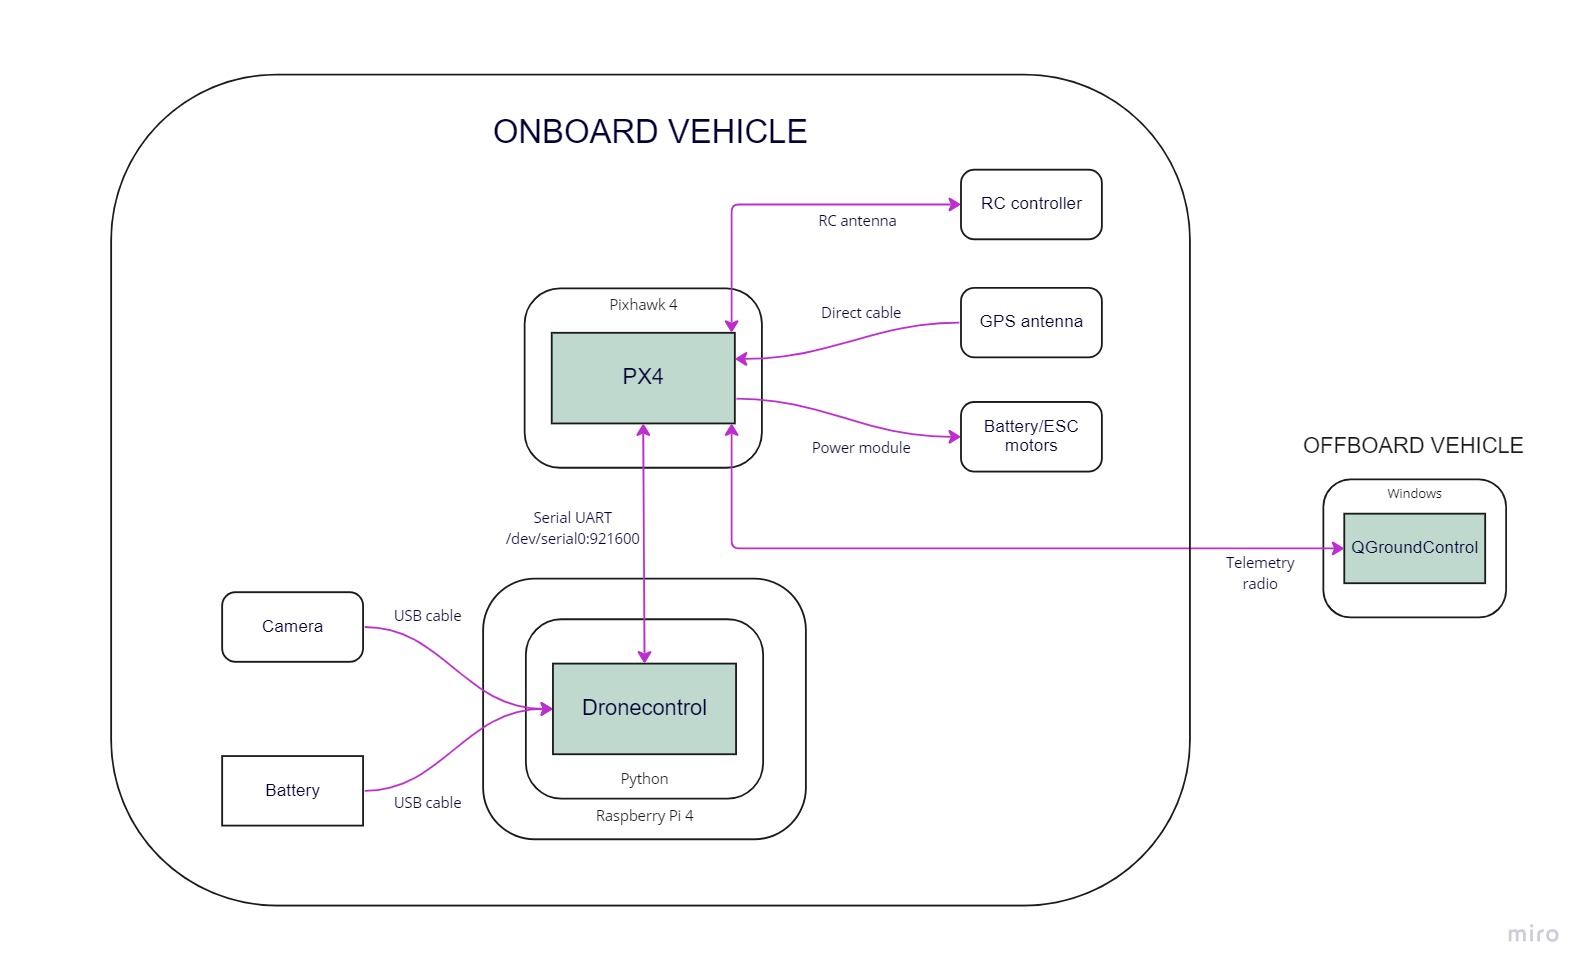
\includegraphics[width=0.85\textwidth,keepaspectratio]{img/onboard-diagram.jpg}
  \caption{Overview of the onboard configuration. All connections are contained inside the vehicle's frame.}
  \label{fig:onboard-config}
\end{figure}


Selecting the appropriate hardware for the onboard computer is crucial in this configuration since the companion computer has to fly along with the flight controller. 
To be able to take into the air, the computer has to be light enough that its weight can be lifted by the propellers while maintaining adequate battery autonomy.
It also needs to be powerful enough that its processor can handle computer vision algorithms.
The Raspberry Pi 4 model chosen for this project and shown in Figure \ref{fig:rpi4-pinout} is one of the most popular small computers available in the market at the time, and it is widely used in all kinds of robotics projects both for education and hobbyists. 
One of the most crucial advantages of using such a platform is the excellent availability of manuals, guides, and other support found on the web. 
In addition, the Raspberry’s officially supported operating
system, called Raspberry Pi OS, is a Debian-based version of Unix, which simplifies the transition from the WSL test environment.

\begin{figure}[H]
  \centering
  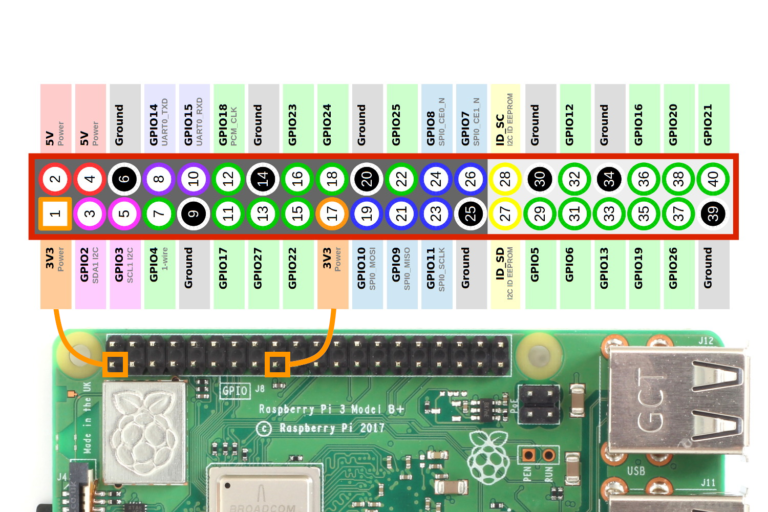
\includegraphics[width=0.8\textwidth,keepaspectratio]{img/rpi4-pinout.png}
  \caption{The Raspberry Pi microcomputer, with its 40-pin GPIO header marked in red and annotated pinout.}
  \source{Adapted from \citetitle{rpi4-pinout} \cite{rpi4-pinout}}
  \label{fig:rpi4-pinout}
\end{figure}

Since this computer is designed for integration with hardware projects, it includes a 40-pin \acrfull{gpio} header (highlighted in Figure \ref{fig:rpi4-pinout}) for connecting external devices.
This pin header, along with the standard ports in the Raspberry Pi, will be used to implement the three connections to the companion computer required for the onboard configuration, shown in Figure \ref{fig:wiring}.
The first connection will provide power to the computer, the second will be a connection to the camera that provides images, and the third one will be the telemetry link to the flight controller.

\begin{figure}
  \centering
  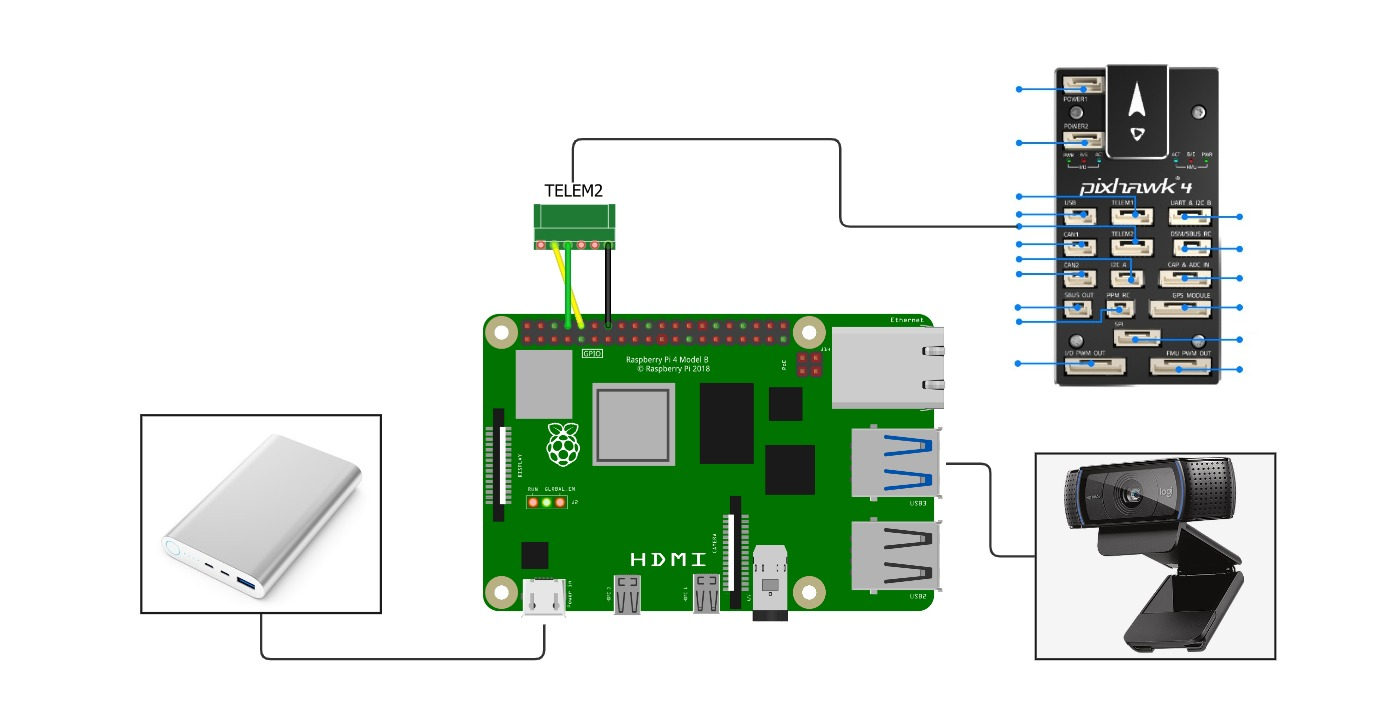
\includegraphics[width=\textwidth,keepaspectratio]{img/wiring-diagram.jpg}
  \caption{A diagram of the wired connections from the Raspberry Pi 4 to the secondary battery and the flight controller (\texttt{TELEM2}).}
  \label{fig:wiring}
\end{figure}

The Raspberry Pi is powered by a 5V input that can be supplied via the USB-C port or specific pins on the GPIO header ("5v Power" on Figure \ref{fig:rpi4-pinout}). 
In the specific vehicle build of this project, the Holybro PM07\footnote{\url{http://www.holybro.com/product/pixhawk-4-power-module-pm07/}} power management board supplies 5V to the flight controller and powers the ESCs for the motors. 
The power management board features two power outputs: one connected to the flight controller's \texttt{POWER1} port and an unused one. 
Initially, attempts were made to power the Raspberry Pi from the main battery by connecting the second output on the power module to the GPIO header's powering pins using a custom connector. 
However, this resulted in an unstable power supply for the Pi board, causing frequent current dips that affected the companion computer's processing capabilities. 
To address this, a secondary battery was introduced, providing power to the Raspberry Pi via a USB to USB-C cable. 
This configuration allows the Raspberry Pi to receive power through its default regulated USB-C port. 
The drawback is the additional weight of the secondary battery, which also needs to be securely attached to the vehicle's frame during flight.

In contrast to selecting a companion computer, the choice of camera for the onboard system offers greater flexibility. The key considerations are lightweight design and straightforward plug-and-play compatibility with the onboard computer. The camera utilized in the tests outlined in section \ref{chap:validation} is the Logitech C920 1080p webcam\footnote{\url{https://www.logitech.com/es-es/products/webcams/c920-pro-hd-webcam.960-001055.html}}. Since the Holybro X500 frame doesn't natively support an onboard camera, a custom mount was designed and 3D-printed using PLA plastic. This mount securely attaches the camera to the underside of the vehicle frame's central rods, ensuring stability during flight. The 3D model of the mount is depicted in Figure \ref{fig:camera-holder-3d}, and the print-ready file is available in the project's repository in GitHub\footnote{\url{https://github.com/l-gonz/tfg-giaa-dronecontrol/blob/main/data/camera-holder.stl}}.

\begin{figure}
  \centering
  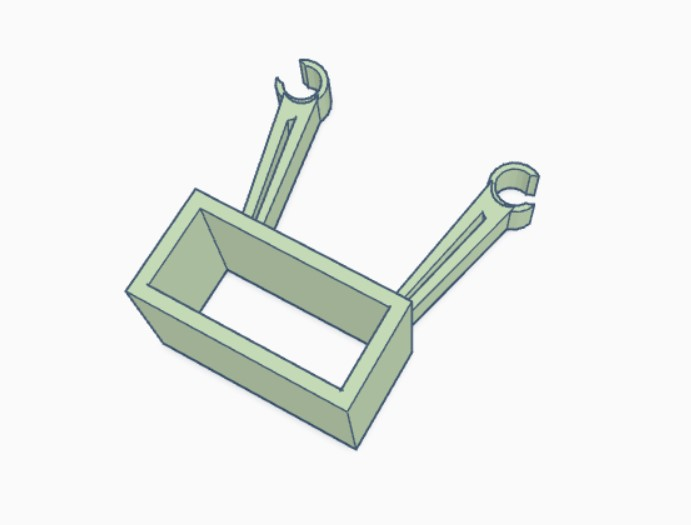
\includegraphics[width=0.6\textwidth, keepaspectratio]{img/cam-holder.jpg}
  \caption{3D model for the camera mount designed for the Holybro X500 frame.}
  \label{fig:camera-holder-3d}
\end{figure}

The last wired connection that needs to be established for this configuration is between the flight controller and the companion computer for MAVLink message exchange.
This connection will use the secondary telemetry port of the flight controller, \texttt{TELEM2}.
Meanwhile, the telemetry radio will remain connected to the \texttt{TELEM1} port to maintain a wireless link.
This link can be employed by a ground station (QGroundControl) to override the companion computer's control during flight.
The telemetry connections on the flight controller use a 6-pin adapter to attach to the \texttt{TELEM} ports.
On the Raspberry Pi side, the other end of the connector has three female Dupont wires that connect to the TX/RX UART pins. The pins in the telemetry port are mapped to the corresponding GPIO pins on the Raspberry Pi's header according to the wiring table provided in \ref{tab:wiring-telem}.
This wiring configuration is also depicted in the diagram in Figure \ref{fig:wiring}.

\begin{table}[ht]
\centering
\begin{tabular}{|ll||ll|}
\hline
\multicolumn{2}{|c||}{\textbf{TELEM2}}                                             & \multicolumn{2}{c|}{\textbf{GPIO header}}                                        \\ \hline \hline
\multicolumn{1}{|c|}{\textit{Pin \#}} & \multicolumn{1}{c||}{\textit{Description}} & \multicolumn{1}{c|}{\textit{Description}} & \multicolumn{1}{c|}{\textit{Pin \#}} \\ \hline
\multicolumn{1}{|l|}{1}               & VCC, +5V                                  & \multicolumn{1}{l|}{}                     &                                      \\ \hline
\multicolumn{1}{|l|}{2}               & TX (out), +3.3V                           & \multicolumn{1}{l|}{GPIO15 (RXD0, UART)}  & 10                                   \\ \hline
\multicolumn{1}{|l|}{3}               & RX (in), +3.3V                            & \multicolumn{1}{l|}{GPIO14 (TXD0, UART)}  & 8                                    \\ \hline
\multicolumn{1}{|l|}{4}               & CTS (in), +3.3V                           & \multicolumn{1}{l|}{}                     &                                      \\ \hline
\multicolumn{1}{|l|}{5}               & RTS (in), +3.3V                           & \multicolumn{1}{l|}{}                     &                                      \\ \hline
\multicolumn{1}{|l|}{6}               & GND                                       & \multicolumn{1}{l|}{GND}                  & 6                                    \\ \hline
\end{tabular}
\caption{Mapping between the \texttt{TELEM2} port in the Pixhawk 4 board and the Raspberry Pi's GPIO header.}
\label{tab:wiring-telem}
\end{table}

By default, the secondary telemetry port, \texttt{TELEM2}, is not enabled for use.
Its configuration can be changed through a ground station computer connected to the Pixhawk board by using the Parameters section of the QGroundControl application.
The specific parameters that need to be set are discussed in section \ref{sec:test-5-rpi}.

% The key parameter that needs to be changed is \texttt{MAV_1_CONFIG}, which configures the serial port a the second instance of MAVLink. Unlike the primary instance (\texttt{MAV_0_CONFIG}), which is set up for telemetry radios, \texttt{MAV_1_CONFIG} should be set to 102 to map to \texttt{TELEM2}. The secondary MAVLink instance is already configured in "Onboard mode" by default, which is the appropriate mode for communication with a companion computer, as opposed to the "Normal mode" used for communication with QGroundControl through \texttt{TELEM1}. Another parameter to consider is \texttt{SER_TEL2_BAUD}, which determines the baud rate of the \texttt{TELEM2} port. The default rate is 921600, suitable for a serial connection. This rate needs to be specified when establishing the connection in the DroneVisionControl application using the MAVSDK library. A comprehensive overview of all the available parameters for board configuration can be found in the PX4 documentation \cite{px4-docs-params}.

Compared to the default baud rate of 57600 used for the telemetry radio link established earlier, the wired serial connection operates at a faster rate of 921600. This means that data can be transferred up to 16 times faster through this link. However, it is important to note that the primary limitation on speed for the program lies in the detection and tracking process running on the images. Therefore, a faster link rate does not necessarily result in an overall performance improvement for the solution. In section  \ref{subsec:performance}, different hardware combinations are analyzed to identify any challenges that may impact the program's performance.

Moving beyond the individual hardware components, it is important to compare the use of this onboard configuration with the previously discussed offboard configuration during testing. While the offboard setup allowed for monitoring the program's output by connecting a screen directly to the companion computer on the ground, such a setup is not feasible in the onboard configuration. However, a solution to this limitation is to leverage the Raspberry Pi's WiFi antenna and configure a remote desktop connection. By connecting to this remote desktop from another computer acting as a ground station, real-time monitoring of the camera output and image recognition can be achieved, along with the capability to provide direct input during flight.
\section{Software architecture}

\begin{figure}
  \centering
  \makebox[\textwidth][c]{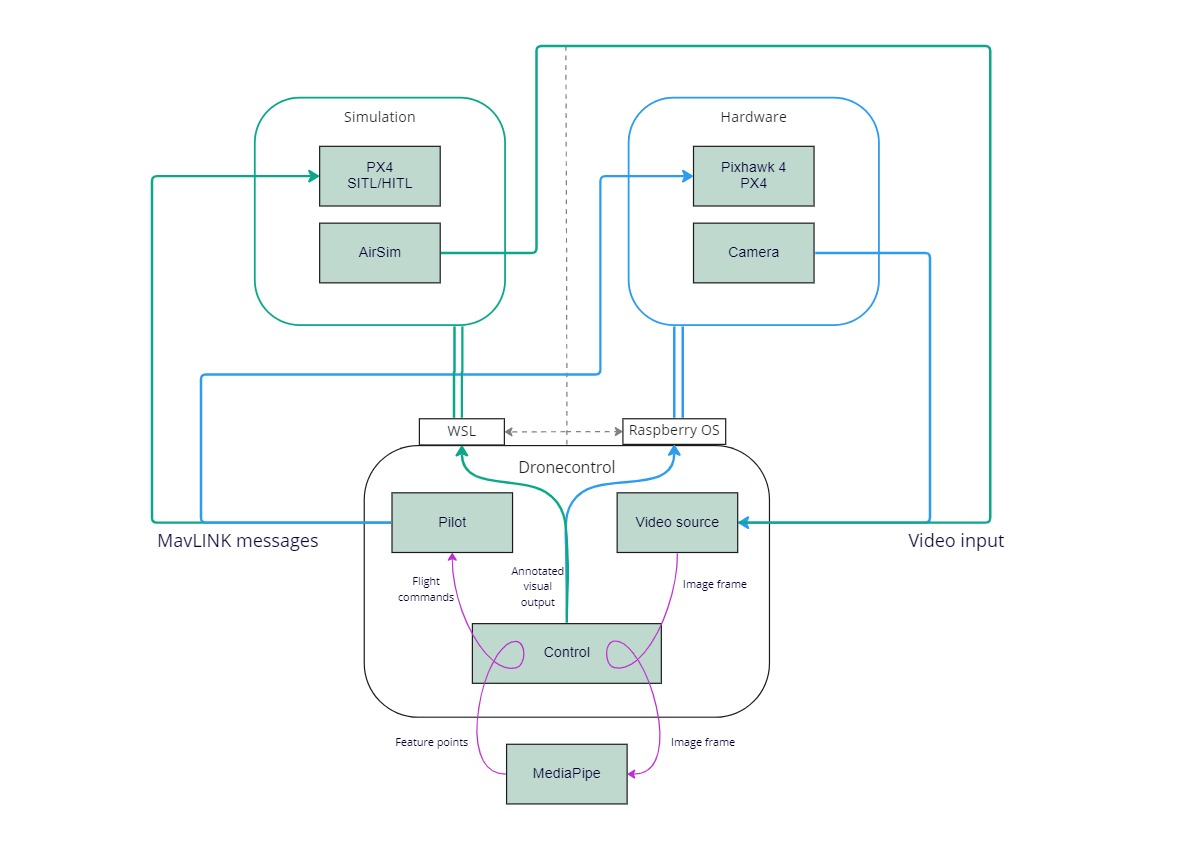
\includegraphics[width=1.2\textwidth, keepaspectratio]{img/software-arch.jpg}}
  \caption{Structure of the DroneVisionControl application main modules (green background) and its interactions with the external components (white background). The information flow is shown in purple arrows for internal communication, green arrows for the simulation environment and blue arrows for hardware interactions.}
\label{fig:soft-arch}
\end{figure}

This section presents the software architecture of the DroneVisionControl application. Except when noted as an external library, all the functionality described has been developed specifically for this project. The complete codebase is located in the linked GitHub repository\footnote{\url{https://github.com/l-gonz/tfg-giaa-dronecontrol}}.
Figure \ref{fig:soft-arch} illustrates the main modules of the designed software and their interactions with external libraries. The application comprises three fundamental parts: the \textbf{pilot module}, responsible for sending instructions to the flight controller and receiving position and state information through the \texttt{mavsdk} library; the \textbf{video source module}, which handles image retrieval from various sources and performs necessary image analysis processing; and the \textbf{control module}, which facilitates interaction between the other two modules to convert pixel information into position points using the \texttt{mediapipe} library, and further into instructions for the pilot.

In the upper part of the diagram in Figure \ref{fig:soft-arch}, the flow of information between the DroneVisionControl application and the external systems is depicted. Green lines represent the path in a simulated workflow, while blue lines indicate the alternative path for a system with actual quadcopter hardware. Purple arrows indicate the input/output of each module within the developed application and how they interconnect. Additionally, smaller utilities have been developed to test the interaction between systems and calibrate different aspects of the control behaviour. These utilities are described in sections \ref{subsec:cam-tool} and \ref{subsec:pid-tools}. A user manual with all the options available in the application can be found in Appendix \ref{app:cli}.

\subsection{Pilot module}
\label{subsec:pilot-module}

The pilot module\footnote{\url{https://github.com/l-gonz/tfg-giaa-dronecontrol/blob/main/dronecontrol/common/pilot.py}} serves the purpose of providing access to the rest of the application for sending and receiving messages from the PX4 controller through the external MAVSDK library. This library offers a simple asynchronous API for managing one or more vehicles, allowing programmatic access to vehicle information, telemetry, and control over missions, movements, and other operations. The integration of MAVSDK with the pilot module utilizes the Python library \texttt{asyncio} \cite{asyncio}, which enables running coroutines in parallel while waiting for messages provided through MAVLink communication.

To interact with the MAVSDK library, all calls need to be written as async functions that await the result of one or more polls to the flight stack. The \texttt{asyncio} library provides support for writing concurrent code using the \texttt{async/await} syntax, serving as a foundation for various Python asynchronous frameworks used for high-performance network and web servers, database connection libraries, and distributed task queues. It offers a set of high-level APIs to run Python coroutines concurrently and grants complete control over their execution.

The pilot module, integrating MAVSDK and \texttt{asyncio}, provides functionality to establish a connection to a PX4 vehicle through a physical serial address or a UDP endpoint.
During this connection phase, the module will poll for internal information from the flight controller to decide when the system is ready to receive instructions.
The MAVSDK library exposes telemetry and other state information through asynchronous generators, defined in Python as a convenient way to retrieve data asynchronously. These are accessed with the \texttt{async\ for} syntax.

The pilot module implements many basic operations that can be executed in the flight controller, along with error handling and safety checks. These operations include takeoff, landing, return home, and manipulating the vehicle's flying velocity directly by providing speeds in body coordinates. These commands can be sent to a vehicle once a connection has been established. 
To enable direct control of the vehicle's velocity, a special flight mode defined by PX4, called Offboard mode\footnote{\url{https://docs.px4.io/main/en/flight_modes/offboard.html\#offboard-mode}}, is required (not related to the offboard configuration described in Section \ref{subsec:offboard}). Offboard mode primarily controls vehicle movement and attitude, adhering to setpoints provided through MAVSDK. This mode relies on position or pose/attitude information available to the flight controller, such as through a gyroscope and a GPS antenna. 
For safety purposes, this mode requires a constant stream of commands to be maintained.
If the message rate falls below 2Hz or the connection is lost, the vehicle will come to a halt and, after a timeout, attempt to land or perform other failsafe actions based on the configured parameters.
This behaviour is handled internally by the MAVSDK library and made available to the application by the pilot module through a \texttt{toggle\_offboard\_mode} function.


As an additional feature, the pilot module also implements an asynchronous queue that can be used to execute actions sequentially. The queue is periodically polled to search for newly added commands to execute, ensuring that each action waits until the previous one has finished and the vehicle is in the desired state before starting the next action. Using this queue is optional and depends on the specific behaviour desired from the control solution. All pilot commands can either be executed immediately, interrupting whichever action is being executed at that time, or be added to the queue to be executed at a later point.


By encapsulating the functionality of sending commands and receiving information from the flight controller, the pilot module provides a robust interface for controlling the vehicle's behaviour and enables seamless integration with other components of the application.


\subsection{Video source module}
\label{subsec:viz-source-module}

The video source module\footnote{\url{https://github.com/l-gonz/tfg-giaa-dronecontrol/blob/main/dronecontrol/common/video_source.py}} aims to provide a collection of classes to retrieve images from different sources in a manner that allows easy interchangeability without affecting the rest of the application. 
This design facilitates testing and adaptability to various environments. Three classes of video sources have been implemented: file, simulator, and camera, all of which inherit from the \texttt{VideoSource} class, as shown in the diagram in Figure \ref{fig:video-source-inheritance}.

\begin{figure}
  \centering
  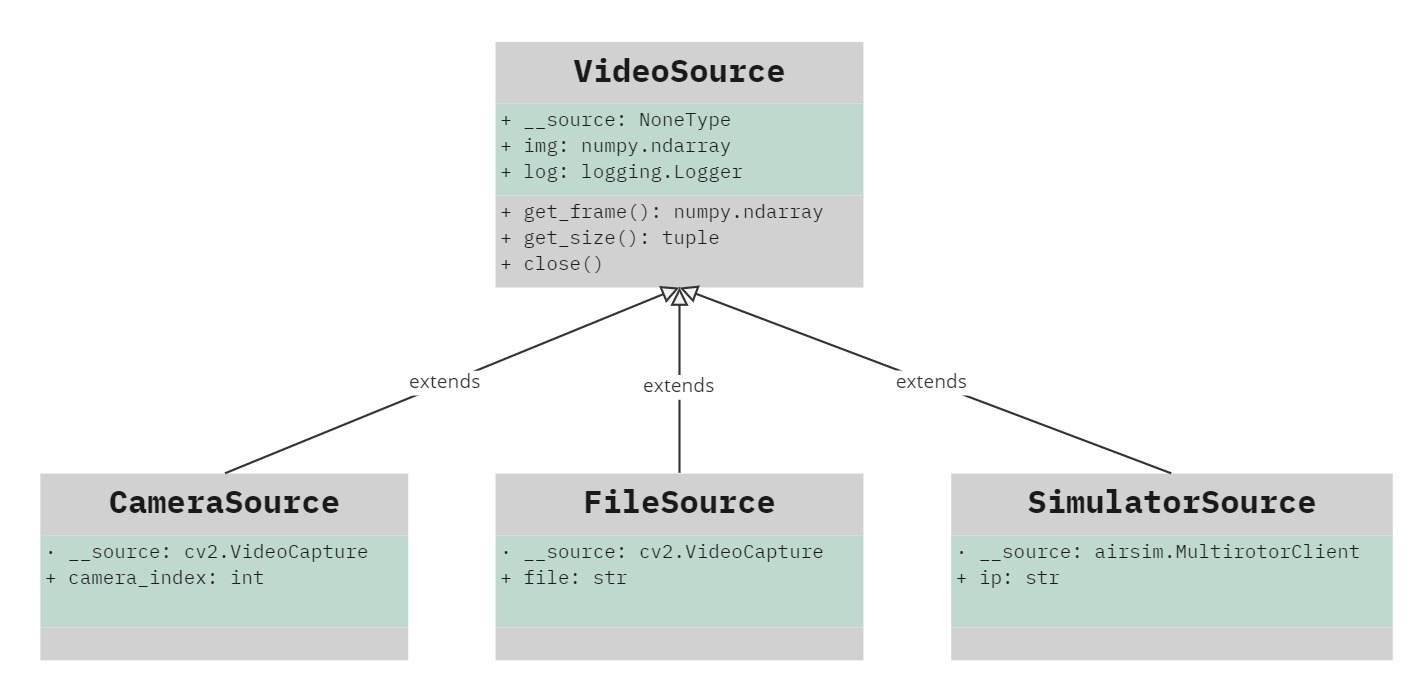
\includegraphics[width=\textwidth, keepaspectratio]{img/uml-video-source.jpg}
  \caption{Diagram of inheritance on the video source classes available to retrieve image data.}
  \label{fig:video-source-inheritance}
\end{figure}

The \texttt{FileSource} class can open a video file stored on the companion computer and provide frames sequentially until the video is completed. This feature enables the replaying image detection algorithms on previously captured videos using the camera tool described in Section \ref{subsec:cam-tool}. The \texttt{CameraSource} class can access a physical camera connected to the computer running the application via USB and provide real-time captured frames. Both the file and camera sources leverage OpenCV's video capture utilities to handle file operations and camera drivers.

The \texttt{SimulatorSource} utilizes AirSim's Python library, \texttt{airlib}, to communicate with the simulator and retrieve images from a camera object attached to the vehicle model in Unreal Engine. It establishes an automatic connection to the simulator via \texttt{localhost}, but it can also be initialized with an IP address to connect to a simulator running on a different computer within the local network. This is particularly useful when the DroneVisionControl runs inside a Linux subsystem (WSL) and the simulator operates on the host Windows system.

\subsection{Vision control module}
\label{subsec:control-module}

The control module encompasses the main logic of the application and is responsible for converting raw images obtained from the video source into commands for the pilot module. Two different types of control solutions have been implemented. The first one is the proof-of-concept control solution described in Section \ref{sec:hands}, operating in the offboard configuration outlined in Section \ref{subsec:offboard}. Its purpose is to translate predefined hand gestures into movement commands for the aerial vehicle. This solution facilitates testing the interaction between all system components in a contained environment by situating the controlling computer outside of the vehicle. The second control system is a follow mechanism, described in Section \ref{sec:follow}, which aims to mimic real-life scenarios where the control algorithms and camera reside onboard the vehicle. It tracks the location of a person detected in the images captured from the drone's perspective and uses that information to calculate velocities necessary for following and keeping the person centred in the drone's view.

Both solutions follow a similar process. Initially, the image is sent to the MediaPipe computer-vision third-party library, described in Section \ref{subsec:mediapipe}, which extracts the required features from the image in the form of 2D coordinates. Subsequently, various calculations specific to each solution are applied to these coordinates to determine the commands sent to the pilot module.
Captured images, detected features and calculated results are communicated to a simple \acrshort{gui}, drawn with the help of the OpenCV library. This interface shows the user all the necessary information about the current state of the running application.

Sections \ref{sec:hands} and \ref{sec:follow} provide further explanations of the control modules used in the two different solutions developed.

\subsection{Camera-testing tool}
\label{subsec:cam-tool}

In addition to the main modules, several utilities have been included in the DroneVisionControl program to facilitate the development and testing processes of the control solutions. The first tool is available in the \texttt{test\_camera} module\footnote{\url{https://github.com/l-gonz/tfg-giaa-dronecontrol/blob/main/dronecontrol/tools/test_camera.py}} and can be accessed through the command \texttt{dronevisioncontrol tools test-camera}. This tool serves multiple purposes, including testing the connection between the computer, the flight stack, and the camera without needing to attach any self-guided control mechanism. It also allows evaluation of the performance of the MediaPipe hand and pose machine learning solutions on real-time images. Additionally, it enables image capture and video recording from a live camera feed for subsequent analysis. 

The test tool can be configured through command-line options to use any of the three available video sources (camera, simulator, or video file), connect to a hardware or simulated PX4 flight controller by specifying a connection string or IP, and run on any system acting as a companion computer. Computer vision can optionally be enabled to process incoming images using hand or pose recognition software. While the tool is running, basic commands such as takeoff, landing, or movement along any direction can be sent to a connected vehicle using the keyboard. Appendix \ref{app:cli} provides a comprehensive breakdown of all the tool's options.

This tool will be used extensively during the tests carried out in Chapter \ref{chap:validation} to validate individual application components in different scenarios without involving complex control mechanisms.

\section{Proof of concept: hand-gesture solution}
\label{sec:hands}
This solution was developed to test that the flow of the application works as expected, both in simulation and in actual flight, and that all the systems can interact and establish the required connections with each other.
For that reason, it is designed to run with as little setup as possible. Flight tests can be undertaken with the minimal hardware components in the offboard configuration (see Figure \ref{fig:offboard-config}).

The control module for this solution is the \texttt{mapper} module\footnote{\url{https://github.com/l-gonz/tfg-giaa-dronecontrol/blob/main/dronecontrol/hands/mapper.py}}.
It runs on a loop that continuously polls for a new frame from the chosen video source and feeds it to the hand detection functionality provided by the MediaPipe library \cite{mp-hands-paper}. If a hand is detected in the image, MediaPipe returns a series of 2D coordinates called landmarks that identify each joint in the hand as depicted in Figure \ref{fig:hand-landmarks}.
The landmarks received from the external library are converted into discrete gestures, such as an open palm, closed fist, or finger pointing in different directions by the developed \texttt{gesture} module\footnote{\url{https://github.com/l-gonz/tfg-giaa-dronecontrol/blob/main/dronecontrol/hands/gesture.py}}. Each detected gesture is then mapped to a command, which is queued to the pilot module and executed once the previous commands have been completed.

\begin{figure}
  \centering
  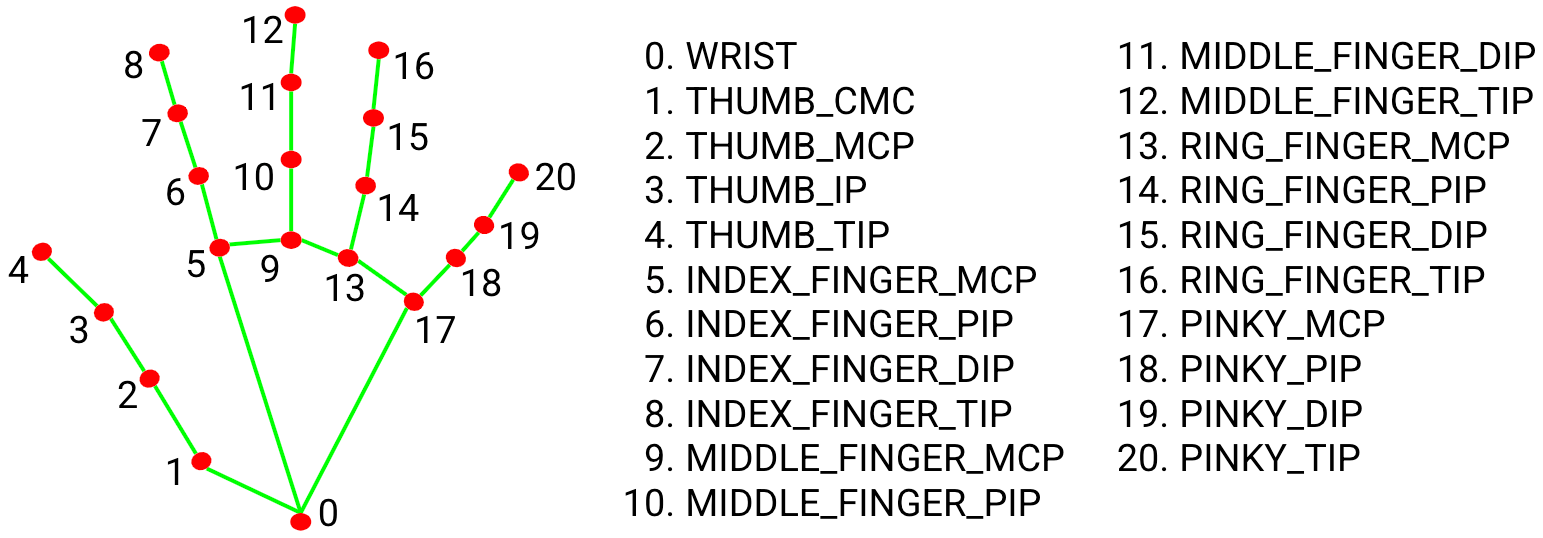
\includegraphics[width=\textwidth, keepaspectratio]{img/hand_landmarks.png}
  \caption{Landmarks extracted from detected hands by the MediaPipe hand solution.}
  \source{Adapted from \citetitle{mp-hands} \cite{mp-hands}.}
  \label{fig:hand-landmarks}
\end{figure}

The conversion from landmarks to gestures performed by the \texttt{gestures} has been designed as a simple but effective way to identify a limited set of hand positions without relying on complex machine-learning solutions. This conversion works by using the landmark coordinates to define two vectors per finger of the hand. One of the vectors points from the base of the hand (wrist landmark) to the base of each finger (points 1, 5, 9, 13, and 17 in Figure \ref{fig:hand-landmarks}), and the other vector points from the base of each finger to its tip (points 4, 8, 12, 16, and 20 in Figure \ref{fig:hand-landmarks}). With the vectors defined, the dot product vector operation is employed to calculate the relative angle of each finger with the base of the hand, as shown in Figure \ref{fig:vector-calcs}. Equations \ref{eq:vectors} and \ref{eq:angles} show example calculations for the index finger.

\begin{eqnarray}
    \vec{a} = P_5 - P_0\;\;\;\;\;\;\;\;\;\;\;\;\;\;\;\; \Vec{b} = P_8 - P_5
    \label{eq:vectors}\\
    \angle (\vec{a}, \vec{b}) = \arccos(\dfrac{\vec{a} \cdot \vec{b}}{\lvert\vec{a}\lvert \lvert\vec{b}\lvert})
    \label{eq:angles}
\end{eqnarray}
\begin{conditions}
\vec{a} &   vector for the index base \\
\vec{b} &   vector for the index finger \\
P_x     &   coordinates of landmark x according to Figure \ref{fig:hand-landmarks} \\
\end{conditions}

\begin{figure}
  \centering
  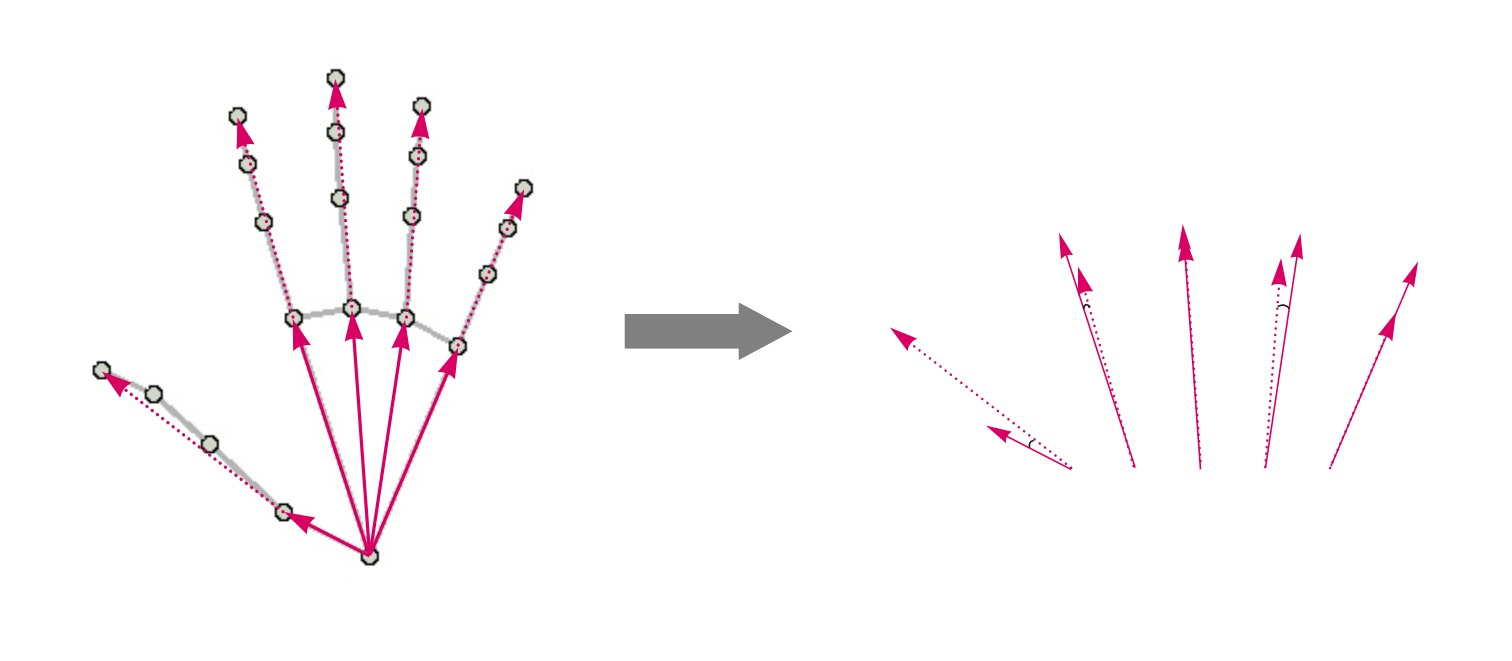
\includegraphics[width=0.9\textwidth, keepaspectratio]{img/hand-vectors.jpg}
  \caption{Vectors extracted from the detected features are used to calculate reference angles to determine hand gestures.}
  \label{fig:vector-calcs}
\end{figure}

By comparing the calculated angles to different thresholds, the module can determine whether each finger is extended or folded and in which direction it points. The thresholds have been determined experimentally by analyzing the angles calculated for the different fingers for different hand positions. Each possible gesture (see Figure \ref{fig:hand-gestures}) is then defined by the direction towards which each finger points, as detailed in the following list:
\begin{itemize}
    \item No hand: this happens when no landmarks can be extracted from the image. As a safety feature, the vehicle stops whichever previous commands it had in its queue and goes into Hold flight mode, hovering in the air while maintaining its position.
    \item Open hand: all five fingers extended, indicating a stop gesture. The drone holds at its current position.
    \item Fist: all five fingers folded into a fist. The drone arms and takes off if on the ground, or lands if already in the air.
    \item Backhand: the back of the hand is shown towards the camera, with the thumb pointing upwards and the other fingers pointing to the side. This gesture puts the drone in Return flight mode, where it climbs to a safe altitude and returns to the last takeoff position.
    \item Index finger pointing up: The index finger is extended and pointing roughly towards the top of the image (within $\pm$30 degrees). The drone enters Offboard flight mode, allowing direct velocity commands. The drone remains in this mode as long as the finger is extended, and its movement can be controlled with any of the next four commands.
    \item Index finger pointing to the right: The index finger points to the right of the image (between 30 and 90 degrees from the top). The drone rolls towards its right side at a speed of 1 m/s.
    \item Index finger pointing to the left: Same as above, but the index finger points to the left of the image. The drone rolls towards its left side.
    \item Thumb pointing to the right: The index finger is extended up (to maintain Offboard flight mode) while the thumb is folded over the palm, pointing towards the right of the screen. This gesture makes the drone pitch forward at a steady speed of 1 m/s.
    \item Thumb pointing to the left: Similar to the previous gesture, but the drone pitches backwards when the thumb points to the left of the screen.
\end{itemize}

\begin{figure}
  \centering
  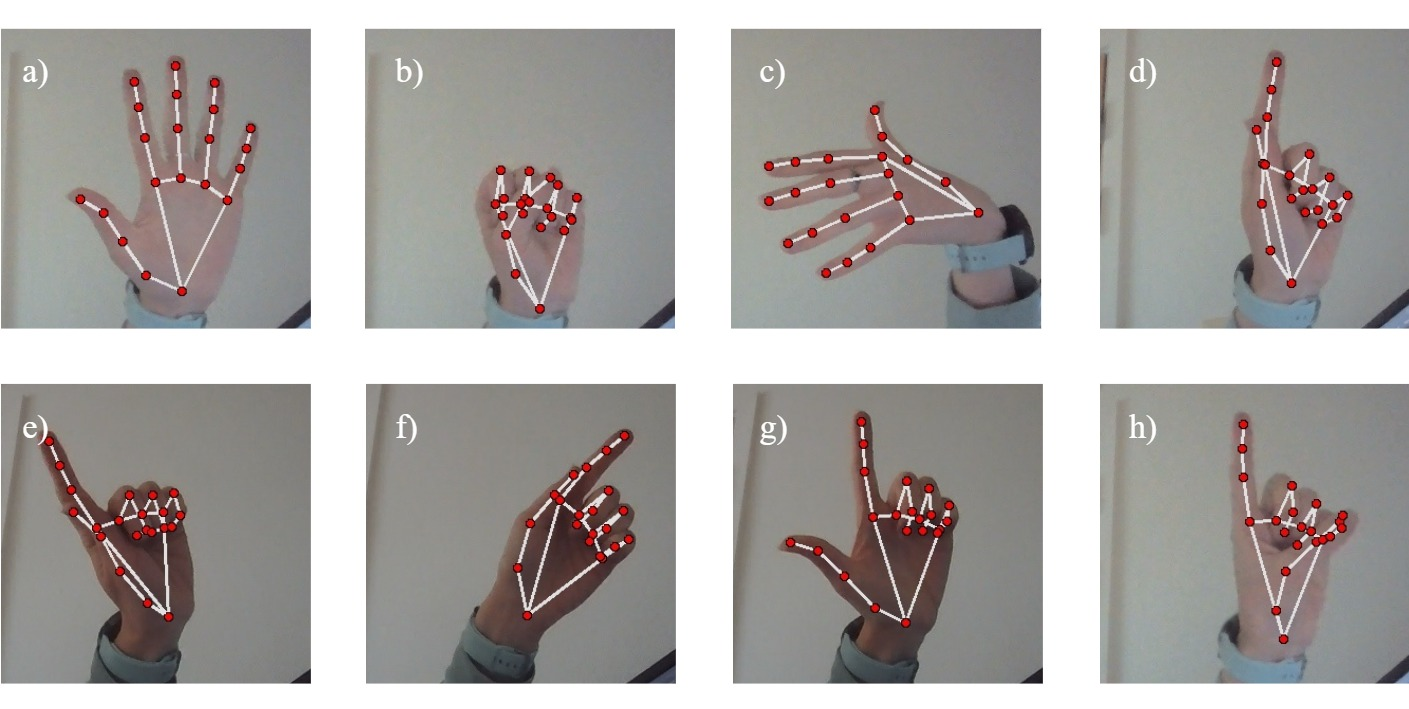
\includegraphics[width=\textwidth, keepaspectratio]{img/hand-gestures.jpg}
  \caption{Gestures detected by the program to control the drone's movement. a) Open hand, b) fist, c) backhand, d) index point up, e) index point left, f) index point right, g) thumb point left, h) thumb point right}
  \label{fig:hand-gestures}
\end{figure}


The program execution is outlined in Figure \ref{fig:hands-loop}.
After all the initial parameters have been set, a secondary thread is started to run the pilot queue detailed in \ref{subsec:pilot-module}, which waits for new commands to be added.
The main thread runs a GUI loop that continuously processes gestures calculated from retrieved images and generates actions that are queued for the pilot.
It also recognizes user input on the keyboard to control the vehicle directly, according to the mapping defined in the \texttt{input} module\footnote{\url{https://github.com/l-gonz/tfg-giaa-dronecontrol/blob/main/dronecontrol/common/input.py}}.


\begin{figure}
  \centering
  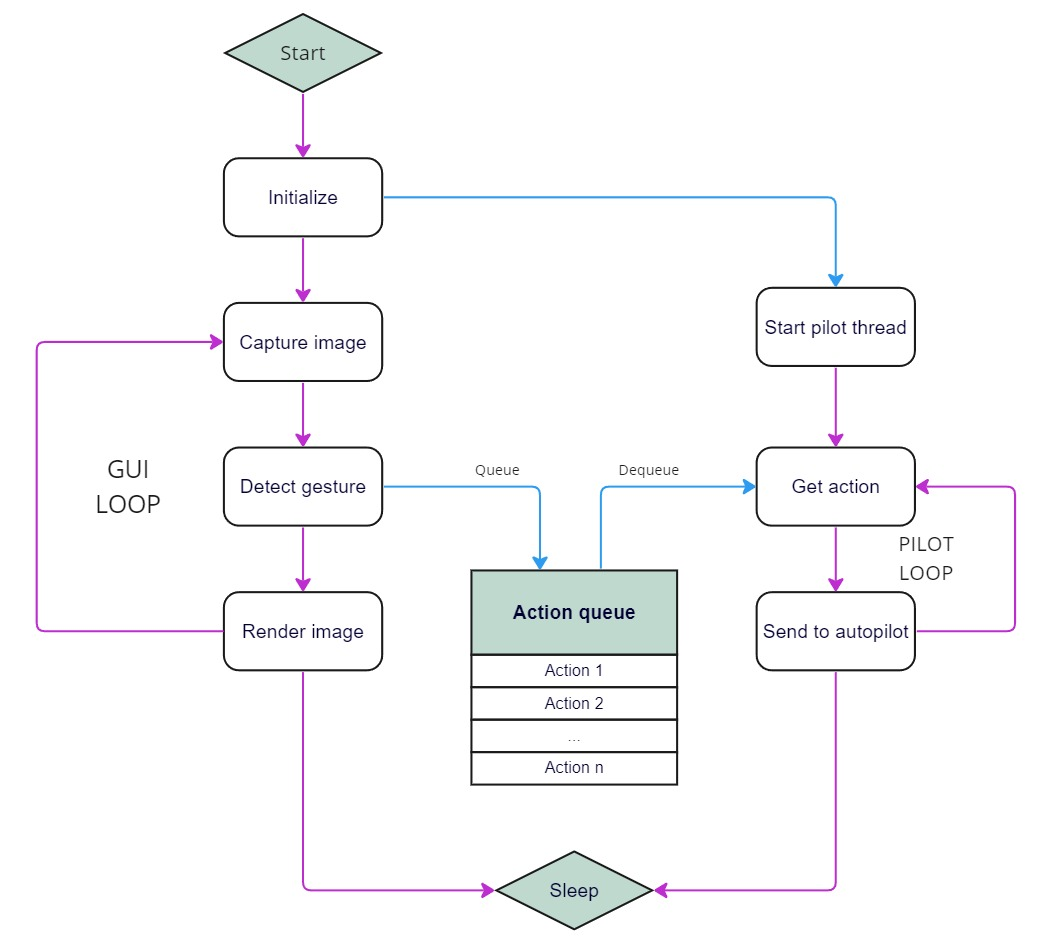
\includegraphics[width=0.8\textwidth, keepaspectratio]{img/hand-loop.jpg}
  \caption{Execution flow for the running loop in the hand-gesture control solution.}
  \label{fig:hands-loop}
\end{figure}

A complete run of this solution is detailed in Section \ref{subsec:fl-test-4}.

\section{Final solution: human following}
\label{sec:follow}

The intention behind developing a UAV control solution that implements tracking and following of humans is to demonstrate the capabilities of the PX4 open-source development platform and its related projects, MAVLink and MAVSDK. The goal is to showcase how complex real-life applications can be designed without relying on expensive proprietary hardware. The follow application requires only a PX4-enabled flight controller installed in an aerial vehicle, a companion computer of appropriate dimensions mounted on board the vehicle, and a camera connected to the companion computer via USB.

In this solution, the vehicle will attempt to detect a single person in its field of view and follow their movements by changing its yaw and forward velocity to match horizontal movements and distance changes, respectively.
During program execution, the drone can be controlled via an RC controller, an external ground station application or keyboard input directly to the companion computer through, for example, a remote shell (SSH) or a desktop sharing program.

For safety reasons, the follow mechanism only engages when the flight mode on the vehicle is changed to Offboard mode. This can be done through a switch in the RC controller configured in QGroundControl for this purpose. The self-guided control also stops automatically if the connection to the computer is lost or any of the available failsafes are triggered, such as low battery or loss of GPS signal. These safety measures are explained in more detail in Section \ref{subsec:safety}.

\begin{figure}
  \centering
  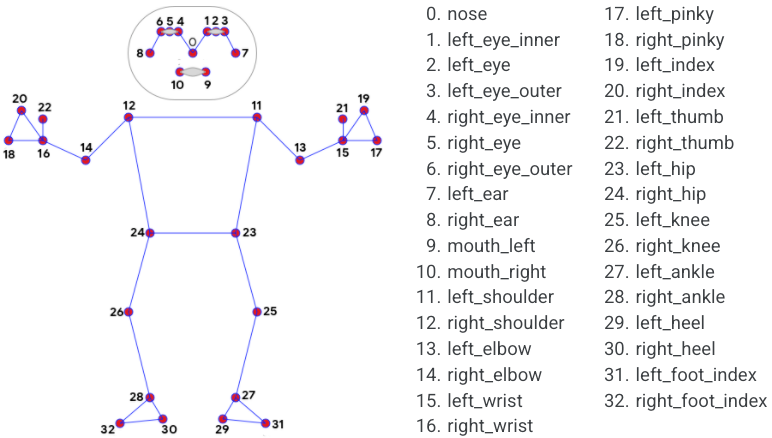
\includegraphics[width=\textwidth, keepaspectratio]{img/pose-landmarks.png}
  \caption{Landmarks extracted from detected human figures by the MediaPipe Pose solution.}
  \source{Adapted from \citetitle{mp-pose} \cite{mp-pose}}
  \label{fig:pose-landmarks}
\end{figure}

When the follow mechanism is engaged, the system continuously retrieves images from the onboard camera. These images are processed using the MediaPipe Pose \cite{mp-pose-paper} computer vision library to extract pose landmarks in the form of 2D coordinates.  Figure \ref{fig:pose-landmarks} shows the features extracted by the external algorithm and their correspondence to the human body. The landmarks received from the MediaPipe library are processed inside the application to draw a bounding box around the detected person and validate that they match the expected pose of a person standing up. The bounding box is calculated as a rectangle with its centre in the midpoint between the minimum and maximum x and y coordinates of the landmarks received and a width and height 10\% bigger than the difference between the maximum and minimum coordinates. There are two additional checks to validate that the landmarks extracted from the external library match a person. The first check simply verifies that the height of the bounding box is greater than its width. The second asserts that the features identified with the head, shoulder, hip, knee, and ankle are situated in the correct order from top to bottom of the image. That is, the y coordinate of the head landmark should always be bigger than the y coordinate of the shoulder landmark, which should in turn be bigger than the y coordinate of the hip landmark. These validation checks are implemented in the \texttt{image\_processing}\footnote{\url{https://github.com/l-gonz/tfg-giaa-dronecontrol/blob/main/dronecontrol/follow/image_processing.py}} module.

\begin{figure}
  \centering
  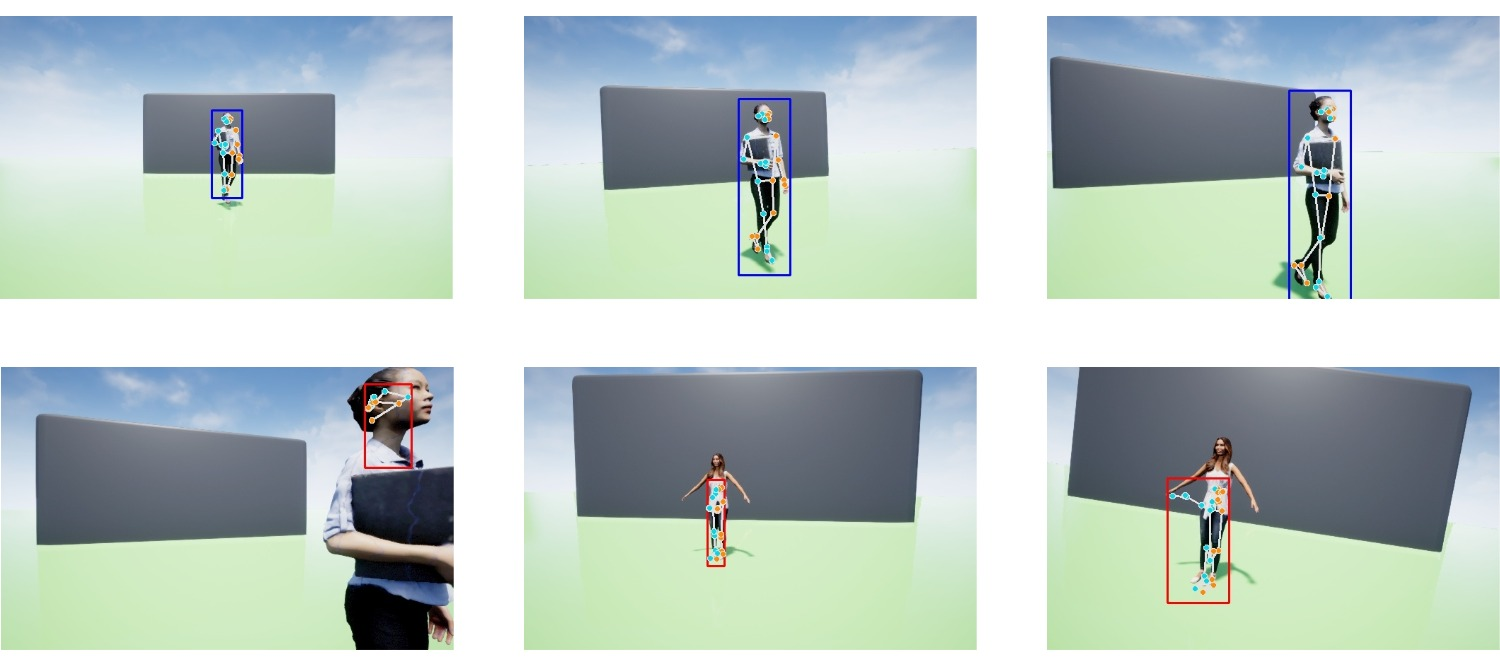
\includegraphics[width=\textwidth, keepaspectratio]{img/pose-validation.jpg}
  \caption{Valid (blue) versus invalid (red) poses detected by the follow solution.}
  \label{fig:pose-validation}
\end{figure}

Figure \ref{fig:pose-validation} shows some examples of the validation checks running on the raw landmarks extracted from an image. Once a valid bounding box is defined around the target person, its position in the image is sent to a control mechanism consisting of two independent PID controllers. These control the vehicle's velocity in the yaw and forward direction, respectively. Section \ref{subsec:pid-tools} describes the mechanisms the PID controllers employ to translate the position of the bounding box to output velocities and how they are customized for the project. To ensure controlled movements, the vehicle will stop and hover if it becomes impossible to detect a person in the image or if the detected features do not match the expected pose (invalid bounding box). The vehicle will resume moving when a valid person is detected again.


The structure for follow solution control module\footnote{\url{https://github.com/l-gonz/tfg-giaa-dronecontrol/blob/main/dronecontrol/follow/follow.py}} is summarized in a diagram in Figure \ref{fig:follow-loop}.
In each execution, after connecting to the pilot module with the starting options provided, the main loop runs continuously until the user quits the program.
For each iteration, an image is retrieved, pose features are extracted, and a bounding box is calculated. If the vehicle is in Offboard flight mode, the calculated bounding box is used as input for the PID controllers, which generate velocity outputs to be sent to the pilot module. Keyboard input is also available to send manual control commands to the vehicle. Unlike in the hand-gesture control solution, all the commands sent here to the pilot module (velocity commands and keyboard input) are run immediately instead of queued for execution.

\begin{figure}
  \centering
  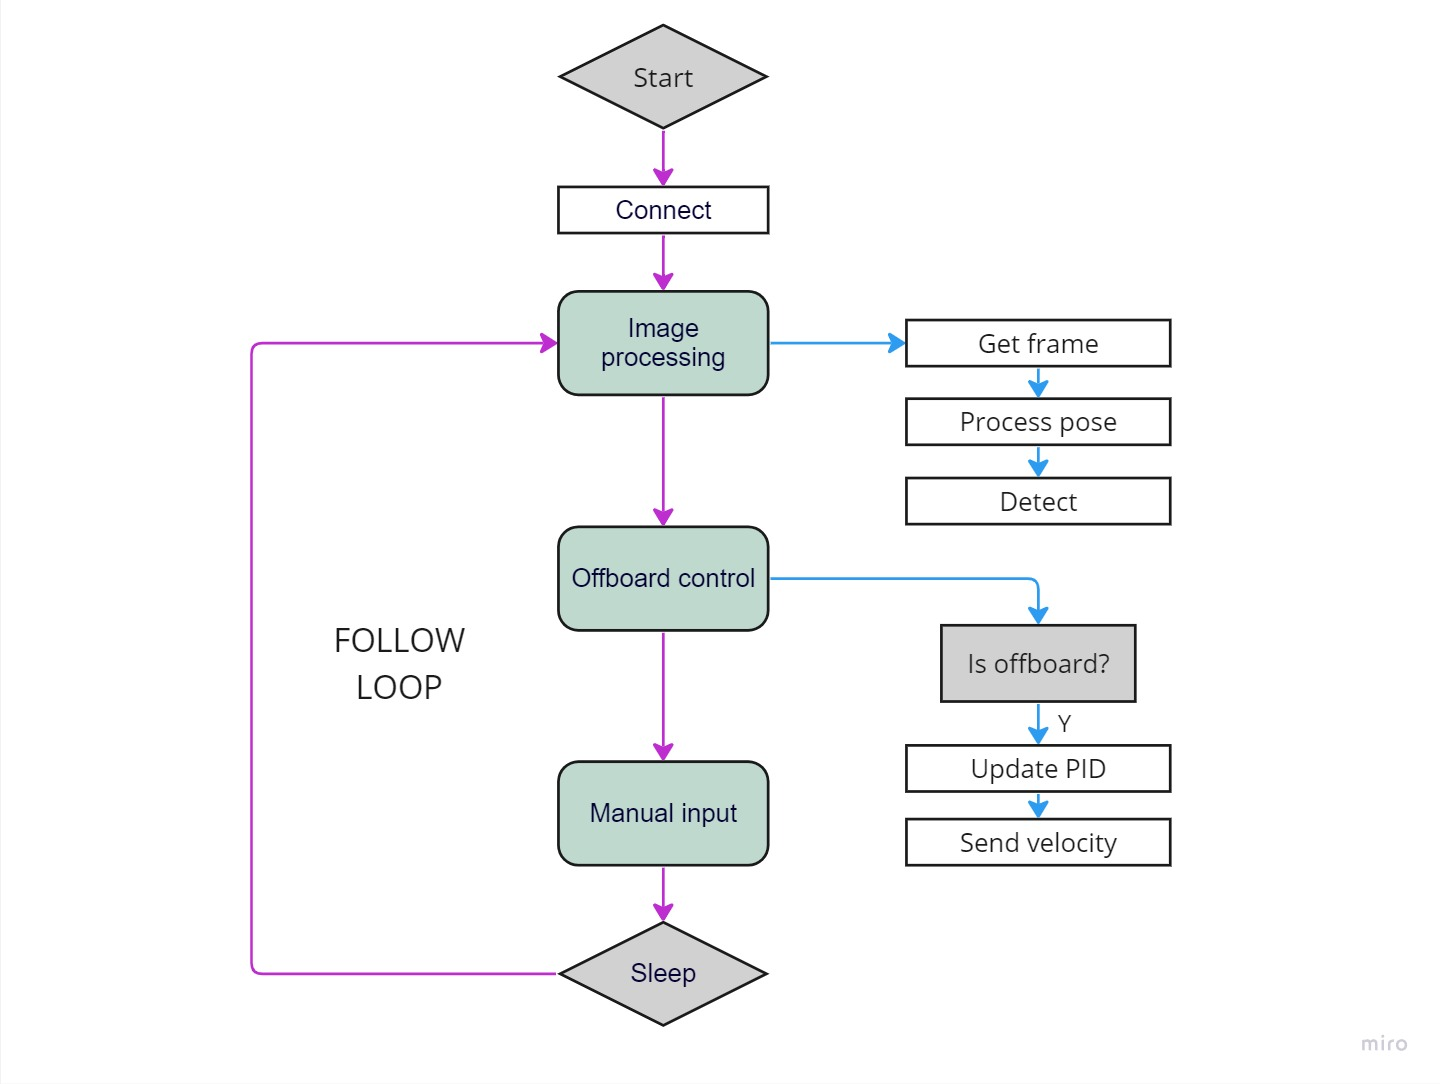
\includegraphics[width=0.9\textwidth, keepaspectratio]{img/follow-loop.jpg}
  \caption{Execution flow for the running loop in the follow control solution.}
  \label{fig:follow-loop}
\end{figure}

A full execution of this solution is shown in flight in Section \ref{subsec:fl-test-5}.


\subsection{PID controllers}
\label{subsec:pid-tools}

A \acrfull{pid} is a control loop mechanism commonly used in systems requiring continuously modulated control. One of its biggest advantages is that it relies only on the response of a single measured process variable, not on knowledge or a model of the underlying process. The controller works by continuously calculating an error value from the difference between the received input on a chosen process variable, which in this case is the detected position of a person in the frame, and the desired set point for that variable, a position centred in the frame. From the error value, the output for the controller is calculated according to Equation \ref{eq:pid}. This output is then fed back into the system as a velocity applied to the vehicle. The change in velocity causes a difference in the detected position, which serves as the next input for the controller, creating a closed control loop.

\begin{equation}
    u(t)= K_p e(t) + K_i \int{e(t)dt} + K_d \frac{de(t)}{dt}
    \label{eq:pid}
\end{equation}
\begin{conditions}
u(t)  &   PID control variable \\
K_p   &   proportional gain \\
K_i   &   integral gain \\
K_d   &   derivative gain \\
e(t)  &   error value \\
de    &   change in error value \\
dt    &   change in time
\end{conditions}

The error value is calculated as the difference between the setpoint $r(t)$ and the process variable or input to the controller, $y(t)$:
\begin{equation}
    e(t)= r(t) - y(t)
\end{equation}

The output obtained from the controller is composed of three individual components. The proportional component, characterized by the proportional gain $K_P$, acts proportionally to the current value of the error. On a P-only controller, there is often a remaining control deviation after an equilibrium is reached which causes the set point not to be reached exactly. The integral component, characterized by the integral gain $K_I$, accounts for past error values, accumulating them over time to eliminate the residual error. The derivative component, characterized by the derivative gain $K_D$, attempts to estimate the future trend of the error by reacting to its rate of change, increasing or dampening the control as the error accelerates or decelerates. Each mentioned gain must be particularized to obtain an effective PID controller for the system under study.

While a PID controller is defined by three control terms, certain scenarios adapt better to using only one or two of these terms to achieve precise control. In such instances, the unused parameters are effectively set to zero, resulting in what is commonly referred to as a PI, PD, P, or I controller, depending on the specific control actions involved. PI controllers are often employed when the derivative action might be susceptible to measurement noise. Nonetheless, the integral term remains crucial in many instances, as it is pivotal in guiding the system towards its intended target value. The process of deciding the control parameters, or tuning, for this particular application is described in Section \ref{sec:test-1-pid}.

As previously mentioned, DroneVisionControl implements two separate PID controllers to control the vehicle's velocity.
The first one is responsible for controlling the yaw velocity of the vehicle, responding to movement in the horizontal axis of the camera's field of view to attempt to keep the person centred horizontally in the field of view. To achieve this, the process variable or input fed to the controller is x-coordinate of the bounding box position in the camera image, normalized to the width of the image, and the setpoint is the middle of the screen (0.5).
The second PID controller directs the forward velocity of the vehicle to respond to changes in the distance between the followed person and the drone. It adjusts the drone's forward movement to keep the height of the bounding box (as a percentage of the total image height) within a desired range. Since the perceived height in the image depends on the camera perspective, the setpoint for this controller should be determined experimentally for each video source. The setpoint for the physical camera used for flight test is decided as 0.5 by analysing images taken during flight as described in Section \ref{sec:test-2-sitl}. In the AirSim simulator, the same 0.5 setpoint for the forward controller maintains the vehicle and the person separated by approximately 4 meters.

Figure \ref{fig:follow-input-calcs} shows how the inputs for each controller are extracted from the coordinates of the bounding box detected around the figure.
\begin{figure}[H]
  \centering
  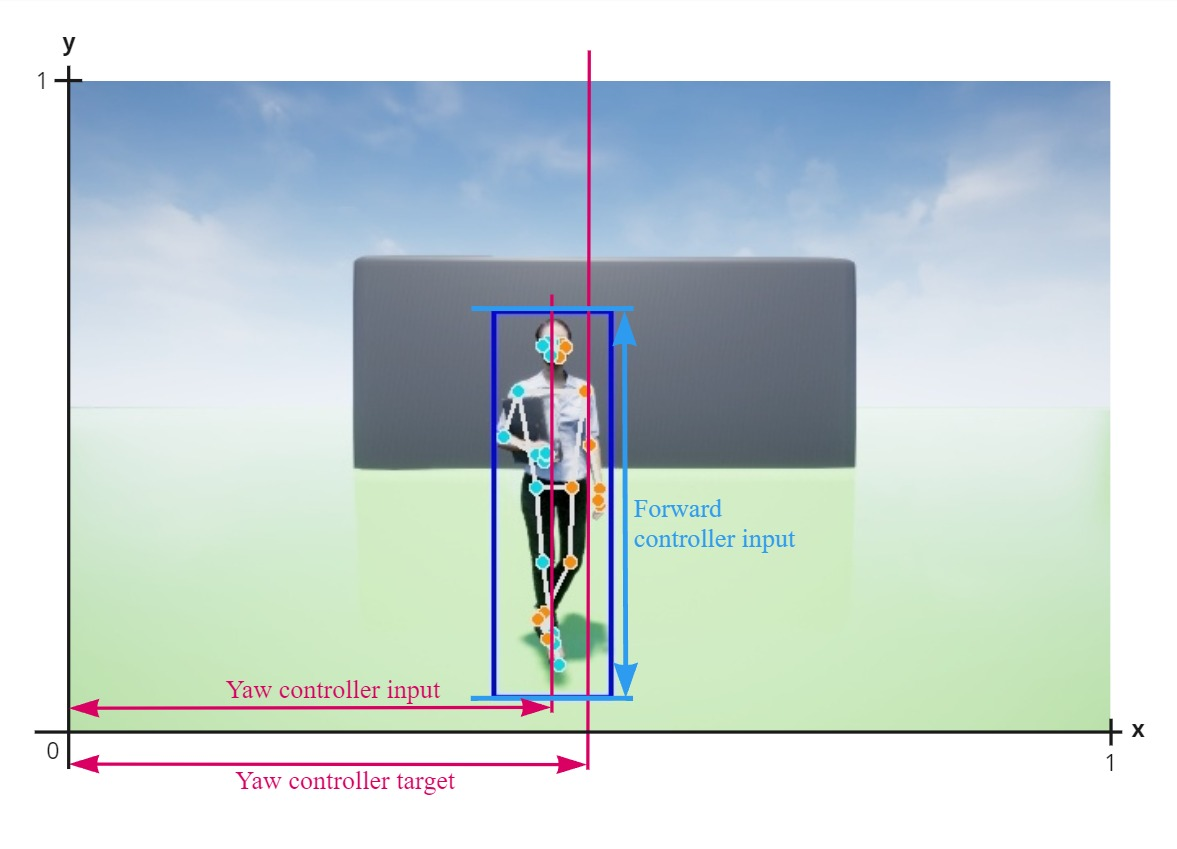
\includegraphics[width=\textwidth, keepaspectratio]{img/pose-calculations.jpg}
  \caption{Calculation of controller inputs from bounding box drawn around the detected figure.}
  \label{fig:follow-input-calcs}
\end{figure}

The velocities that the controllers output are sent to the pilot module to be communicated to the autopilot through MAVLink messages. However, these velocities do not exactly match the speeds measured by the vehicle's telemetry. The autopilot includes its own internal controllers that translate received commands into signals for the propeller motors to run at a specific speed and maintain a smooth flight. This additional step between the output of the controllers in DroneVisionControl and the vehicle's actual speed will have to be taken into account when the control parameters are determined. In practice, it will result in the possibility of implementing more aggressive behaviour on the controllers, as the more complex internal autopilot controllers will end up smoothing the final trajectory.

The PID controllers in this project are implemented with the help of the open source \texttt{simple-pid} Python library \cite{pid-library}, which supplies all the necessary calculations.
It is only necessary to provide the coefficients or tunings ($K_P$, $K_I$, $K_D$) and the set point (target value) for the controller at the start and then update it periodically with the current input value to receive the output velocity.
In the DroneVisionControl application, it is the internal \texttt{controller} module\footnote{\url{https://github.com/l-gonz/tfg-giaa-dronecontrol/blob/main/dronecontrol/follow/controller.py}} the one that interacts with the external \texttt{simple-pid} library to feed and receive the correct values to the PID controllers calculated from the bounding box around the detected person.

\subsubsection{PID tools}
An additional utility called \texttt{tune\_controller}\footnote{\url{https://github.com/l-gonz/tfg-giaa-dronecontrol/blob/main/dronecontrol/tools/tune_controller.py}} has been developed for tuning and testing the response of the PID controllers. Tuning a PID controller typically involves testing different combinations of coefficients empirically. The \texttt{tune\_controller} tool facilitates this process by allowing users to specify a range of potential coefficients and testing the system's response using images retrieved from AirSim and a simulated flight controller (SITL or HITL). The tool sets up a simulated person in an offset position from the target centre, engages the controller with the test values, and plots the detected position input and calculated velocity output on a graph for analysis. After each test, the vehicle returns to the starting position to reset the environment for the next coefficient to be checked. The tool can be executed using the command \texttt{dronevisioncontrol tools tune} and can be started with the option \texttt{--yaw} or \texttt{--forward} to tune a specific controller while deactivating the other one. Each coefficient can be tested individually by providing fixed values for the other two parameters.


\subsection{Safety measures}
\label{subsec:safety}

The DroneVisionControl application implements a very experimental vision-based guidance system.
Therefore, to carry out flight tests in real-life conditions, it is necessary to ensure that there are sufficient safety mechanisms to prevent accidents. The software-based safety features used in this project can be divided into those offered by the external PX4 autopilot and those developed as part of the DroneVisionControl application.

The PX4 autopilot offers various safety configuration options, known as failsafes, documented in \citetitle{px4-docs-safety} \cite{px4-docs-safety}. These failsafes detect undesired conditions during flight and include detecting a lost connection to the companion computer while in Offboard mode, a loss of RC transmitter link or GPS position, low battery levels during flight, and unexpected flipping of the vehicle. When any of these conditions are detected, the autopilot triggers a flight mode change to either Hold (hover) or Return (fly back to takeoff position and land), ensuring the safety of the drone and its surroundings. The failsafes' failure conditions and actions triggered in response can be configured through QGroundControl, the PX4 console or an offboard API (MAVSDK).

Additionally, operator control can play a vital role in ensuring safety during flight by leveraging QGroundControl to map PX4 commands to switches in an RC controller. This allows the operator to use an RC controller with a configured switch to deactivate Offboard mode at any time during a flight controlled by the follow solution. This action causes the vehicle to disregard instructions from the companion computer and assume control through GPS-assisted or manual flight modes. A secondary switch can also be configured as a kill switch, allowing for an immediate stop of all motor outputs when needed. This feature is particularly useful in situations where the vehicle is on the ground and has trouble taking off to reduce the risk of propeller damage if the vehicle flips.

On the DroneVisionControl side, the computer vision module that interacts with the external pose detection library incorporates several checks to validate that the received results match specific features associated with a standing human figure. Any detections that do not pass these tests are rejected as invalid as described in \ref{sec:follow}. If the detection output is invalid or empty (nothing detected in the image) is received, the vehicle immediately enters Hold flight mode. In this mode, any velocity commands are discarded, and the drone hovers in its current position. When a valid person is detected again, the follow mechanism resumes controlling the vehicle's velocity. In addition to detection validation, the application incorporates safety measures related to the PID controllers and the pilot module, which limit the maximum possible velocity of the vehicle at all times during the execution. The PID controllers have output limits set within DroneVisionControl to prevent abnormal velocity commands from being sent to the flight controller.


By integrating the safety features of PX4 with those developed for this project, the DroneVisionControl application aims to mitigate potential risks and ensure safe flight operations under real-life conditions.

% \clearpage

% EXPERIMENTOS Y VALIDACIÓN %
\chapter{Experiments and validation}
\label{chap:validation}

This chapter outlines the validation process for each essential component required for the proper functioning of the entire system, ranging from initial simulation tests to comprehensive flight tests conducted on the final guidance solution. The validation process follows the order depicted in Figure \ref{fig:validation-chart}.

The first section involves testing the integrity of the different components in the simulated environment. Initially, there is a component testing section where each part is tested individually. Afterwards comes the integration testing, where the SITL simulation of the PX4 flight controller is integrated with the AirSim environment and the DroneVisionControl offboard application to validate the exchange of control commands and images for the detection software.

In the second section, the simulation tools are employed to tune the PID controllers that drive the behaviour of the follow control solution. The purpose of the tuning process is to find good enough values for the control parameters to be able to validate the vision control solution and determine the limits of the simulation tools. During the process, first, the response of each of the two controllers will be analysed individually and then they will be integrated together to ensure that work in a satisfactory manner.

In the third section, once the software is proven to adhere to the established safety requirements, the simulation is moved to the HITL mode, where the software runs on dedicated hardware instead of on the simulation computer. This hardware includes the autopilot board Pixhawk 4 and the Raspberry Pi as its companion computer. The main goal is to verify that all the communication channels function as expected and that the devices deliver the required performance.

Lastly, in the fourth and final section, a series of flight tests are carried out, gradually increasing in complexity. These tests span from basic manual control of the vehicle using an RC controller to fully autonomous target-following flight executing in the complete system.

\begin{figure}
  \centering
  \makebox[\textwidth][c]{
  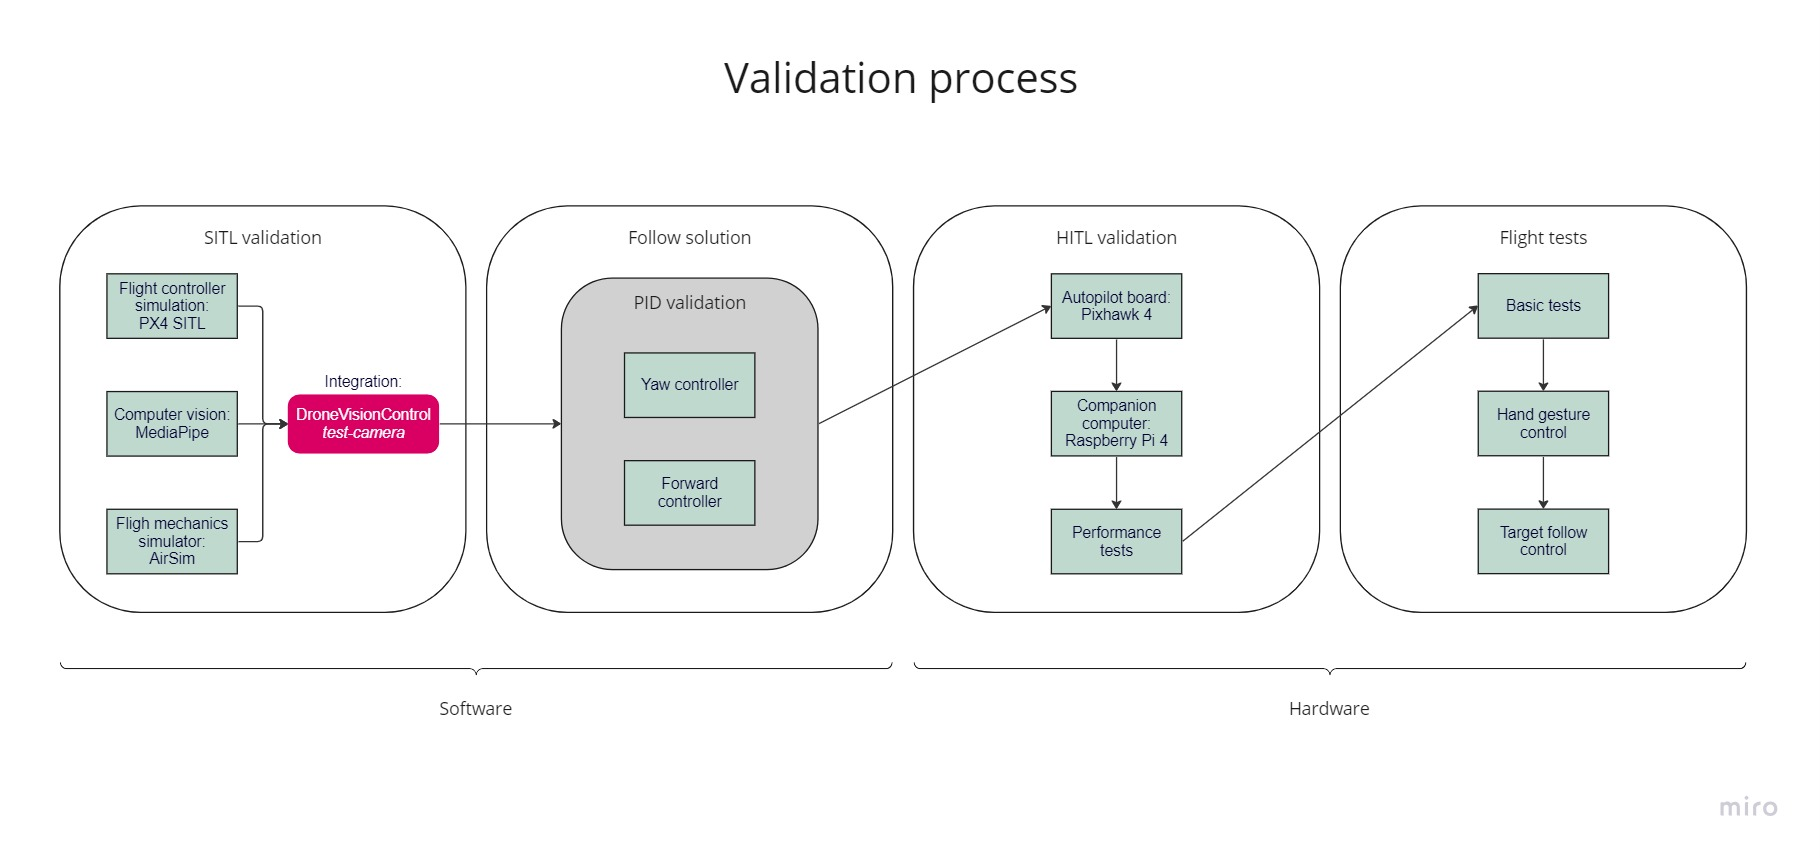
\includegraphics[width=1.2\textwidth, keepaspectratio]{img/validation-chart.jpg}}
  \caption{Summary of the validation process followed in this chapter.}\label{fig:validation-chart}
\end{figure}
\todo[inline]{Fix up diagram a bit to match phase 2 (Title: PID design, green boxes: Tuning process, Validation process; inside first (grey): yaw and fwd)}

\section{PX4 SITL simulation and validation}
\label{sec:test-2-sitl}

Section \ref{sec:devenv} describes the software-in-the-loop simulation mode developed by PX4.
Using this mode makes it possible to test and validate the correct operation of each part in the program's architecture.
To start, it is necessary to validate that it is possible to use the connection between the simulated flight controller and the DroneVisionControl program to send commands to the simulated vehicle, as well as to capture images from a connected camera and use them to test the detection algorithm.
The full list of validation steps is, therefore:
\begin{enumerate}
    \item Verify that it is possible to start the simulated flight controller and that it connects to the 3D simulator vehicle.
    \item Connect the DroneVisionControl program to the flight controller and send basic commands.
    \item Retrieve images from a camera and run computer vision detection on them.
    \item Integrate the last three steps by running the hand-gesture control solution described in section \ref{sec:hands}
\end{enumerate}

For this purpose and to be able to run with a minimal configuration, the Gazebo simulator\footnote{\url{https://gazebosim.org/home}} included with the base PX4 installation will be used as the 3D environment.
This simulator works inside Linux on the same computer that runs the SITL PX4.
To be able to later transition into using the AirSim simulator instead, which runs in Windows, with minimal changes, for this test, PX4, Gazebo and the DroneVisionControl program will run inside the Windows Subsystem for Linux.
The complete installation process necessary to run these tests is explained in appendix \ref{app:install-dev-env} and \ref{app:install-dronecontrol-rpi}.

\begin{figure}
  \centering
  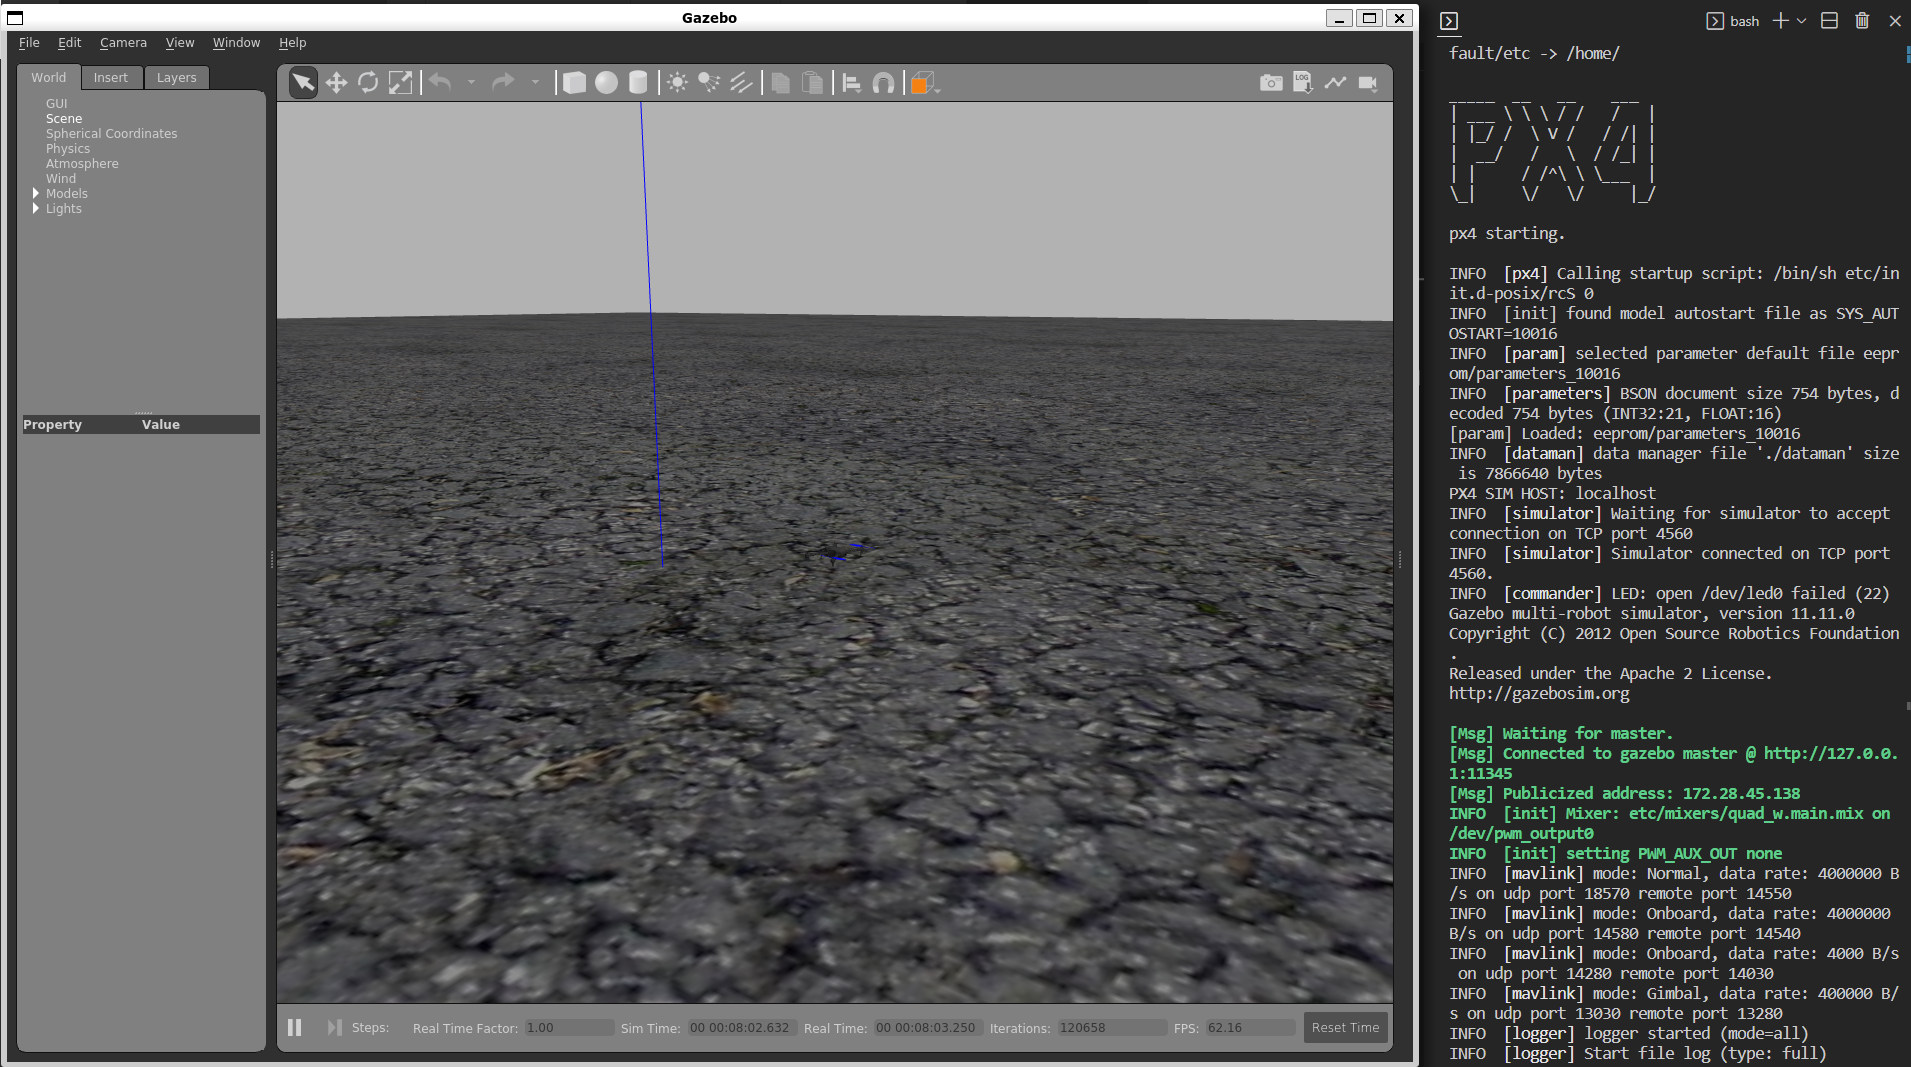
\includegraphics[width=\textwidth, keepaspectratio]{img/gazebo.png}
  \caption{Gazebo simulator (left) and output from the PX4 terminal (right) after PX4's software-in-the-loop mode is started}\label{fig:gazebo}
\end{figure}

Once both parts are installed, PX4 and Gazebo can be started by running the \texttt{make\ px4\_sitl\ gazebo} command inside its installation folder.
The result of this command can be seen in figure \ref{fig:gazebo}, where the left part shows the user interface and 3D world of the Gazebo simulator and the right side contains the PX4 console that can be used for sending commands and changing the configuration parameters of the simulated flight controller.
The most straightforward command to test is takeoff, which is done by sending \texttt{commander takeoff} through the console.
Figure \ref{fig:gazebo-takeoff} shows the simulator's state after the takeoff command, where the vehicle model has climbed to the default height of 2.5 meters above the ground.
The command to land the vehicle again is \texttt{commander land}.

\begin{figure}
  \centering
  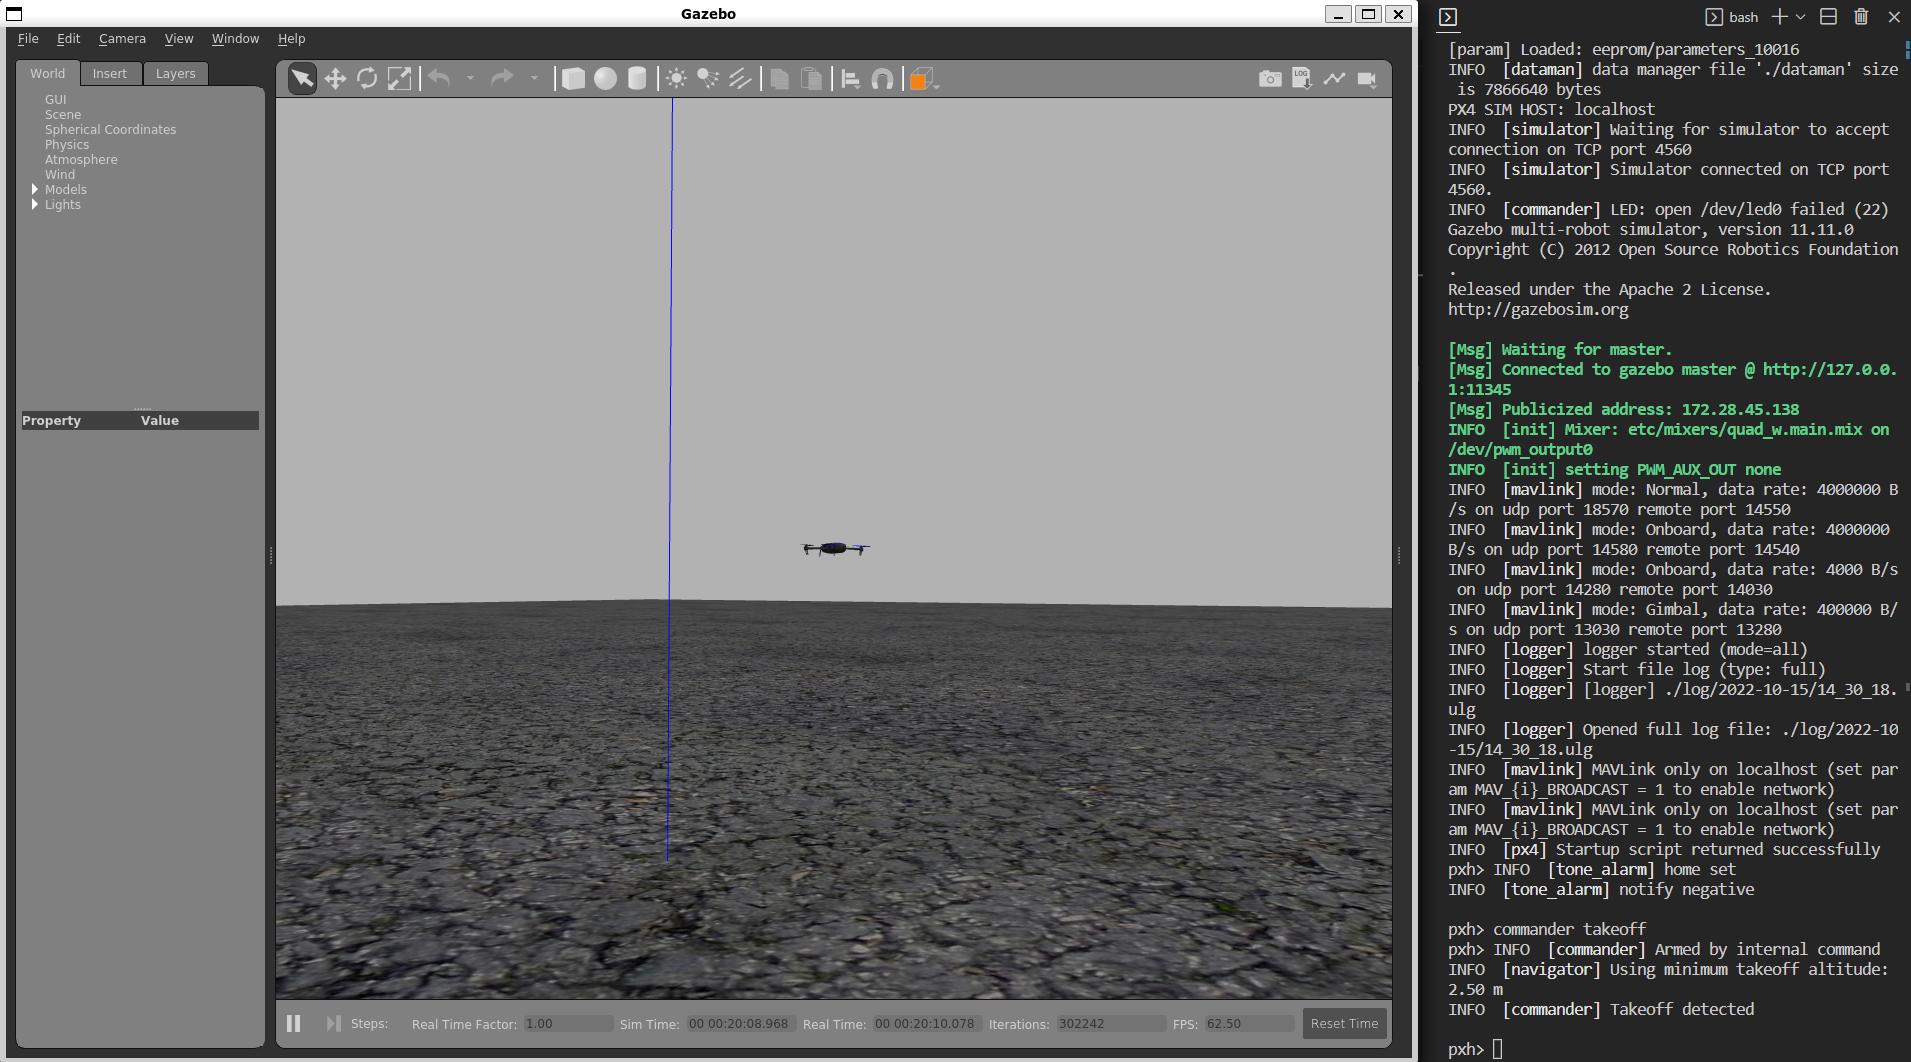
\includegraphics[width=\textwidth, keepaspectratio]{img/gazebo-takeoff.png}
  \caption{Gazebo simulator (left) and output from the PX4 terminal (right) after the takeoff command has been executed}\label{fig:gazebo-takeoff}
\end{figure}

The next step is to connect the DroneVisionControl application.
The camera testing tool described in section \ref{subsec:cam-tool} has been developed specifically for this test so that it is possible to establish a connection to PX4 SITL and process images without engaging any of the program's control modules.
The commands are then sent to PX4 through keyboard input.
For example, the key "T" will make the simulated vehicle take off.
Figure \ref{fig:sitl-hand} shows the image and text output of the program when the test camera tool is run with the hand detection feature activated.
On the left side, the detection algorithm tracks the joint of the hand present in the captured image and on the right side, the logged information shows when the connection is established and keyboard commands are sent to the simulator.


\begin{figure}
  \centering
  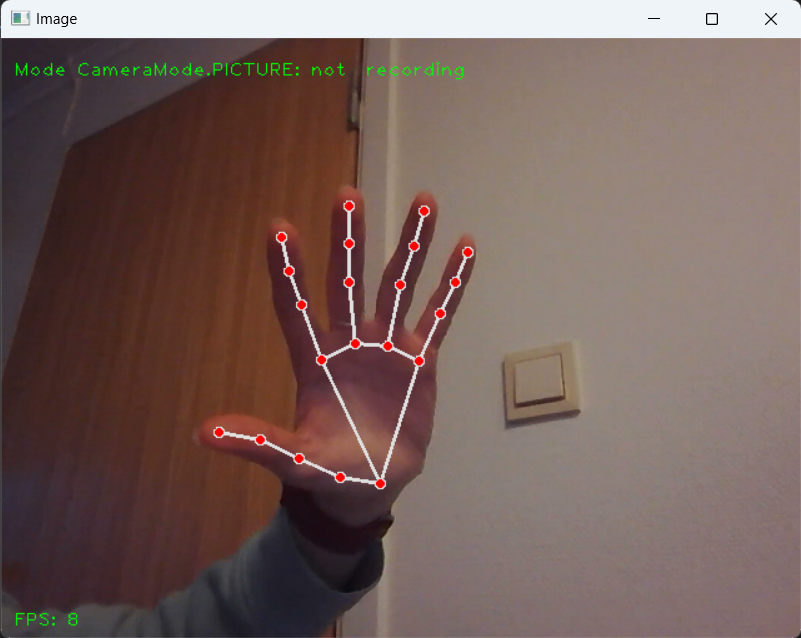
\includegraphics[width=\textwidth, keepaspectratio]{img/sitl-hand.png}
  \caption{Hand detection algorithm running on images taken from the computer integrated webcam}\label{fig:sitl-hand}
\end{figure}

The entire execution of a test of the hand-gesture-based control solution is shown in this \href{https://l-gonz.github.io/tfg-giaa-dronecontrol/videos/test-sitl-hand}{video}\footnote{\url{https://l-gonz.github.io/tfg-giaa-dronecontrol/videos/test-sitl-hand}} in this link and an image extracted from it can be seen in figure \ref{fig:sitl-hand-video}.

\begin{figure}
  \centering
  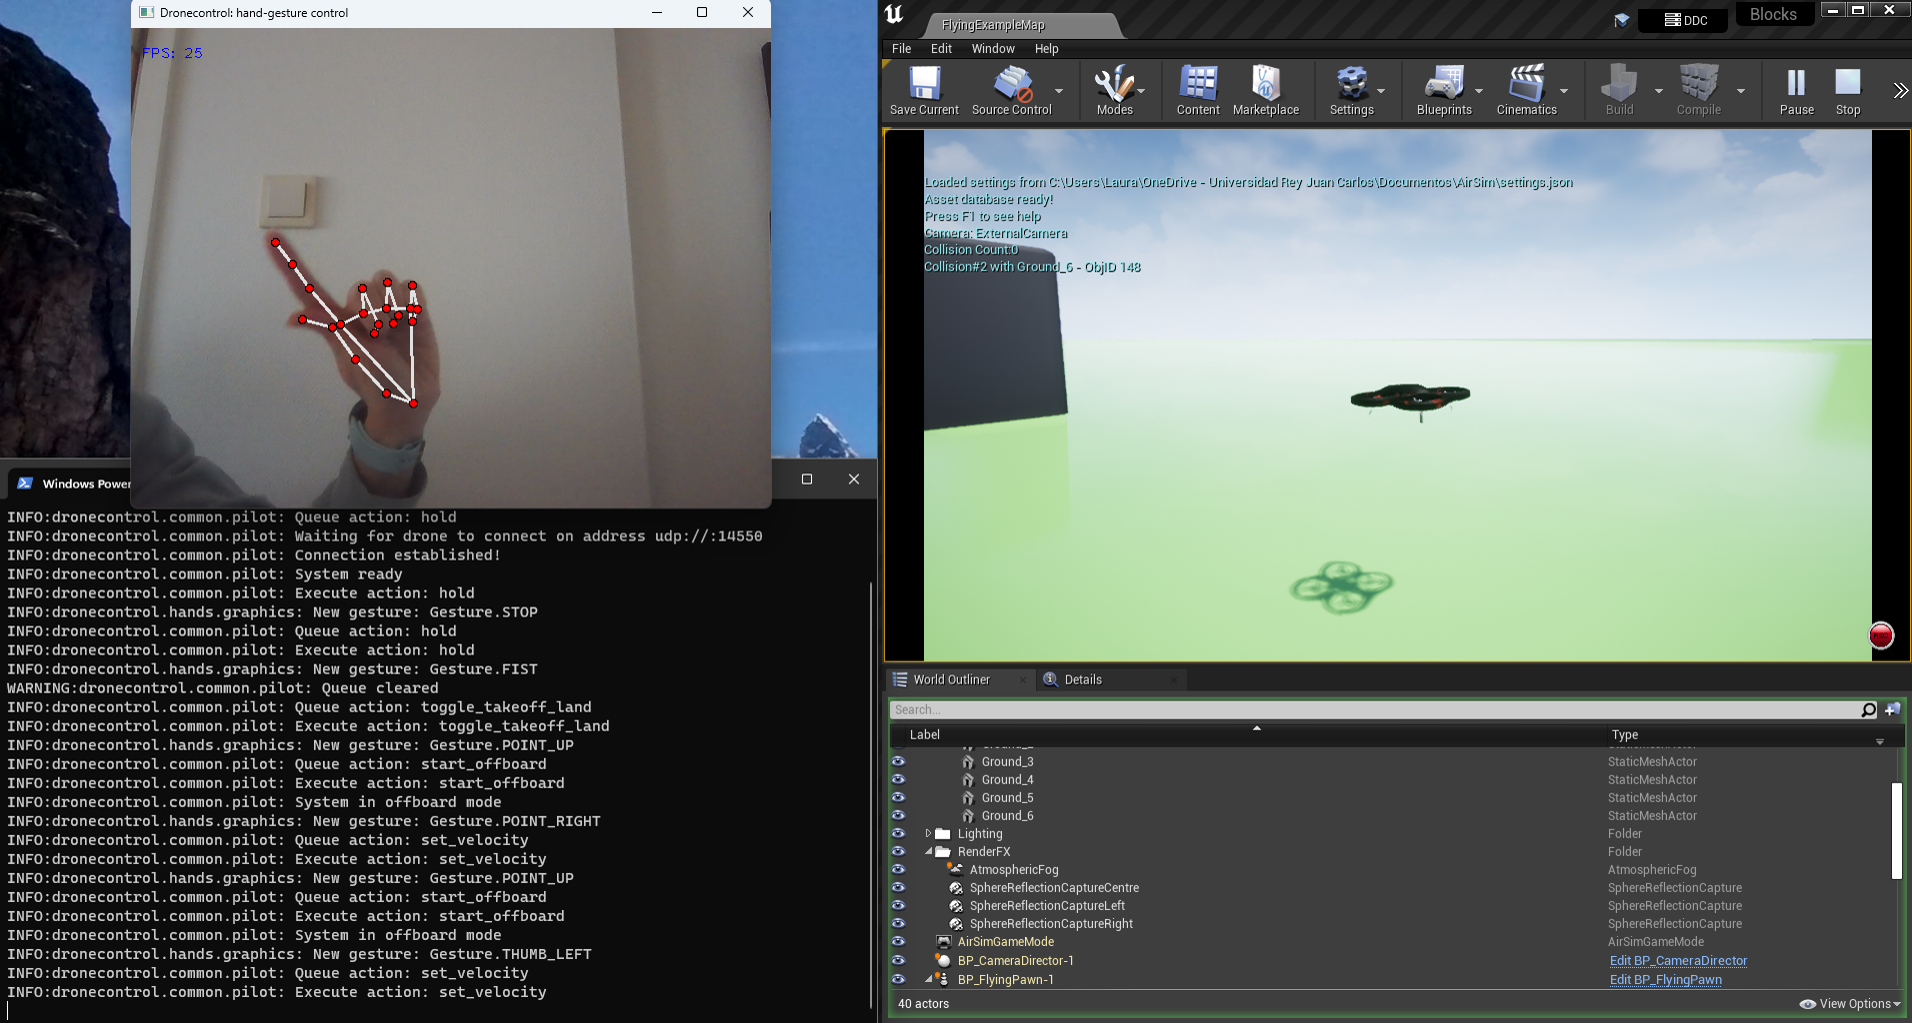
\includegraphics[width=\textwidth, keepaspectratio]{img/video-hand-sitl.png}
  \caption{Single frame from the video showing the full execution of the hand-gesture control solution}
  \label{fig:sitl-hand-video}
\end{figure}


\subsection{PX4 SITL validation with AirSim}
\label{sec:test-3-airsim}

The end goal for the testing environment is for it to use the AirSim simulator to take advantage of its 3D-world and computer vision capabilities.
For this reason, it becomes necessary to validate that the new simulator can run correctly on Unreal Engine on the computer and interact with PX4 as well as it did with the default Gazebo simulator and that all the necessary features for detection, tracking and following work as expected.
All these characteristics will be checked in the order below:
\begin{enumerate}
    \item Verify that the AirSim simulator can start, connect to the PX4 SITL through the WSL virtual network and receive commands from the PX4 terminal.
    \item Check that the DroneVisionControl program can connect to both AirSim through the WSL network to receive images and PX4 through the local network to send movement commands.
    \item Test the pose recognition algorithms on the images obtained from the AirSim simulation.
    \item Check that the follow solution can control the vehicle's velocity directly in PX4's offboard mode.
\end{enumerate}

In the first place, the AirSim simulator needs to be installed in the Windows host.
The complete installation process is described in appendix \ref{app:install-dev-env}.
There are specific configuration parameters that have to be set to be able to connect the AirSim simulator in Windows to the PX4 SITL running inside WSL.
On the simulator side, AirSim's settings file has to include a line defining the IP address of the network interface to use.
This parameter, along with the entire configuration file used for SITL testing, can be found in appendix \ref{app:airsim-config}.
On the PX4 side, it is necessary to specify that the simulator will attach through a different IP address than \texttt{localhost}.
This is done by setting the \texttt{PX4\_SIM\_HOST\_ADDR} environment variable in the Linux system to the IP address of the Windows host on the WSL virtual network before starting PX4 as follows:
\begin{minted}{bash}
export PX4_SIM_HOST_ADDR=[IP-address]
make px4_sitl none_iris
\end{minted}
This starts the software-in-the-loop execution, which attempts to attach to an already running simulator listening on the IP address specified and the TCP port 4560, in this case, AirSim.
Therefore, every time either PX4 or AirSim stops its execution, both of them have to be restarted in the specific order of first the AirSim simulator and then the PX4 flight controller.
Figure \ref{fig:airsim-sitl} shows the testing environment after the AirSim simulator and the PX4 console have been started successfully.

\begin{figure}
  \centering
  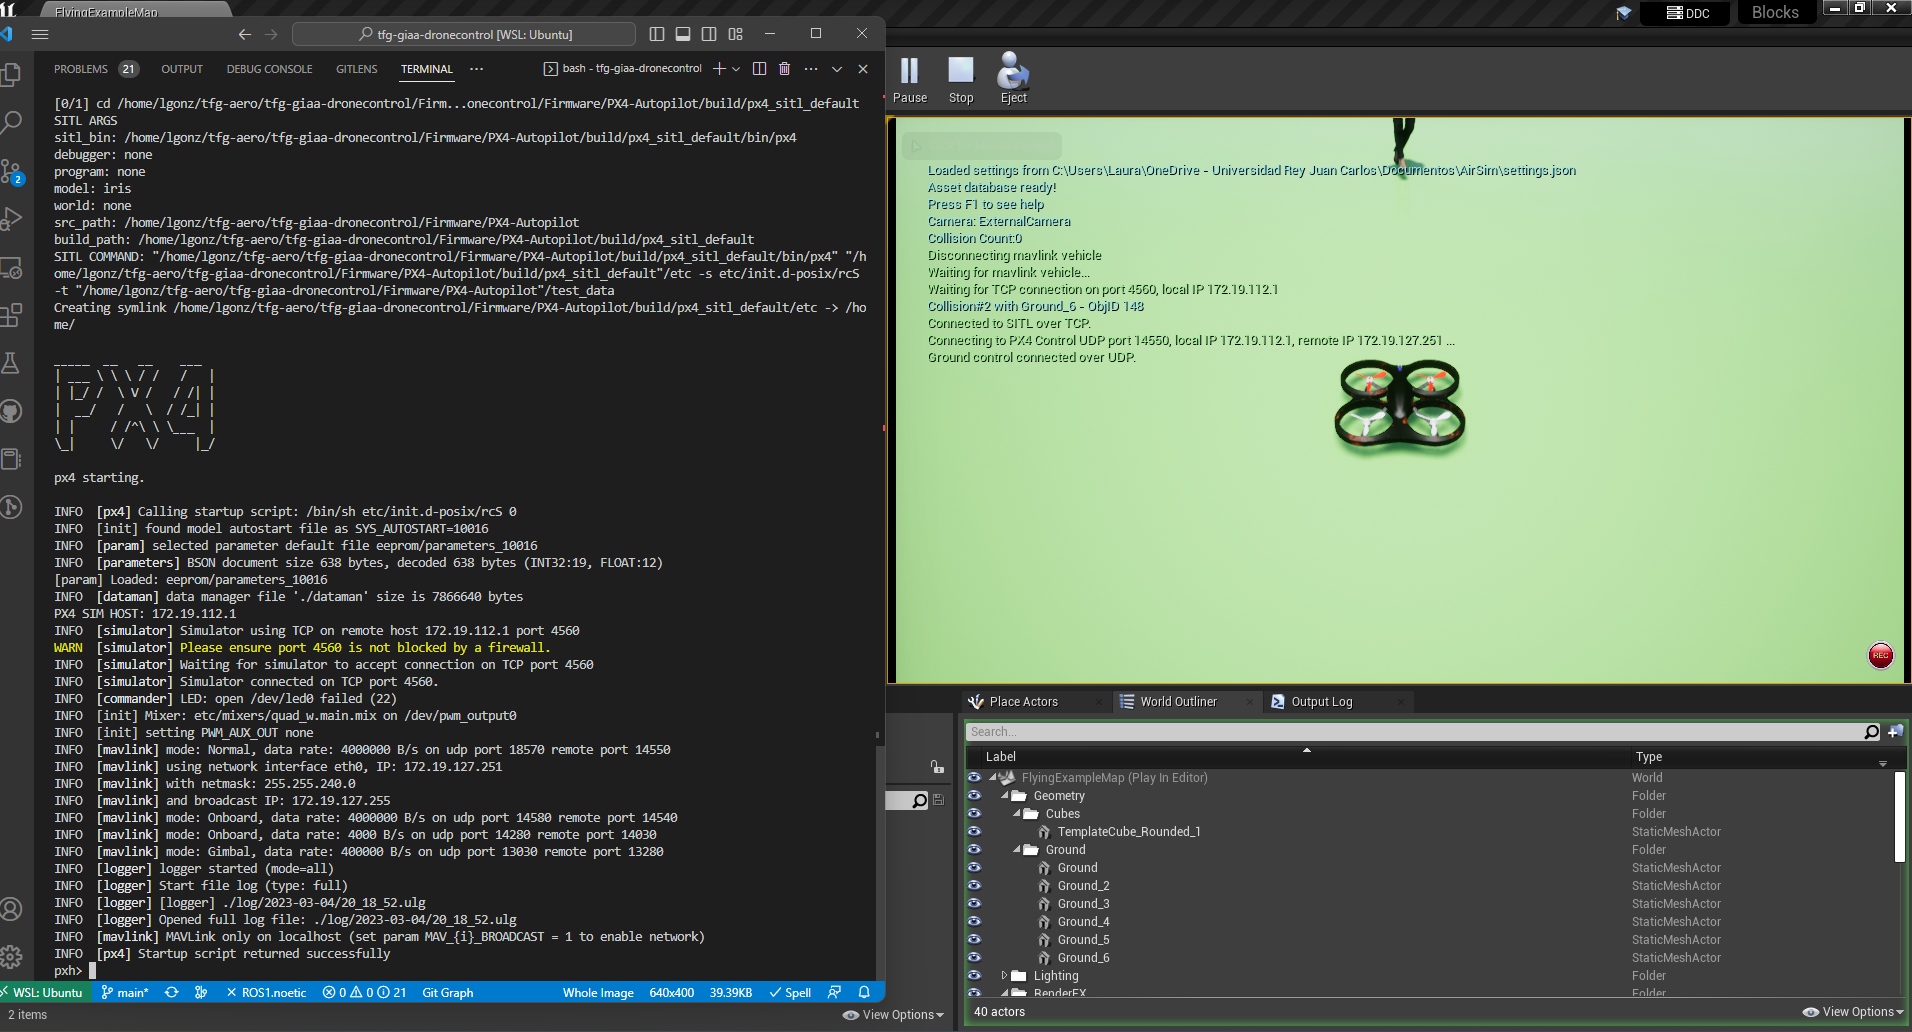
\includegraphics[width=\textwidth, keepaspectratio]{img/airsim-sitl.png}
  \caption{AirSim environment connected to PX4 flight stack running in SITL mode}
  \label{fig:airsim-sitl}
\end{figure}

At this point, it is possible to use the PX4 console to send takeoff and land commands to the simulator and observe the 3D model of the vehicle climb into the air.
To test the detection and tracking of human figures from images taken inside the simulator, one can again use the camera testing tool provided with DroneVisionControl.
Figure \ref{fig:airsim-sitl-pose} shows the output when the tool is run with a 3D model of a person situated in front of the drone in the simulated world and the command:
\mint{bash}{dronevisioncontrol tools test-camera --wsl --sim --pose-detection}
In the image, the computer vision utility detects the main features of the human body and a bounding box is drawn around it.
Meanwhile, the logged output from the program shows two calculated positions in the terminal: the x coordinate of the midpoint of the bounding box and the percentage of the image height covered by the height of the bounding box.
These two numbers are the inputs for the PID controllers used in the follow solution as described in section \ref{sec:follow} so that the output can be used to calibrate the distance from which the drone is to follow the person when that control mode is engaged.

\begin{figure}
  \centering
  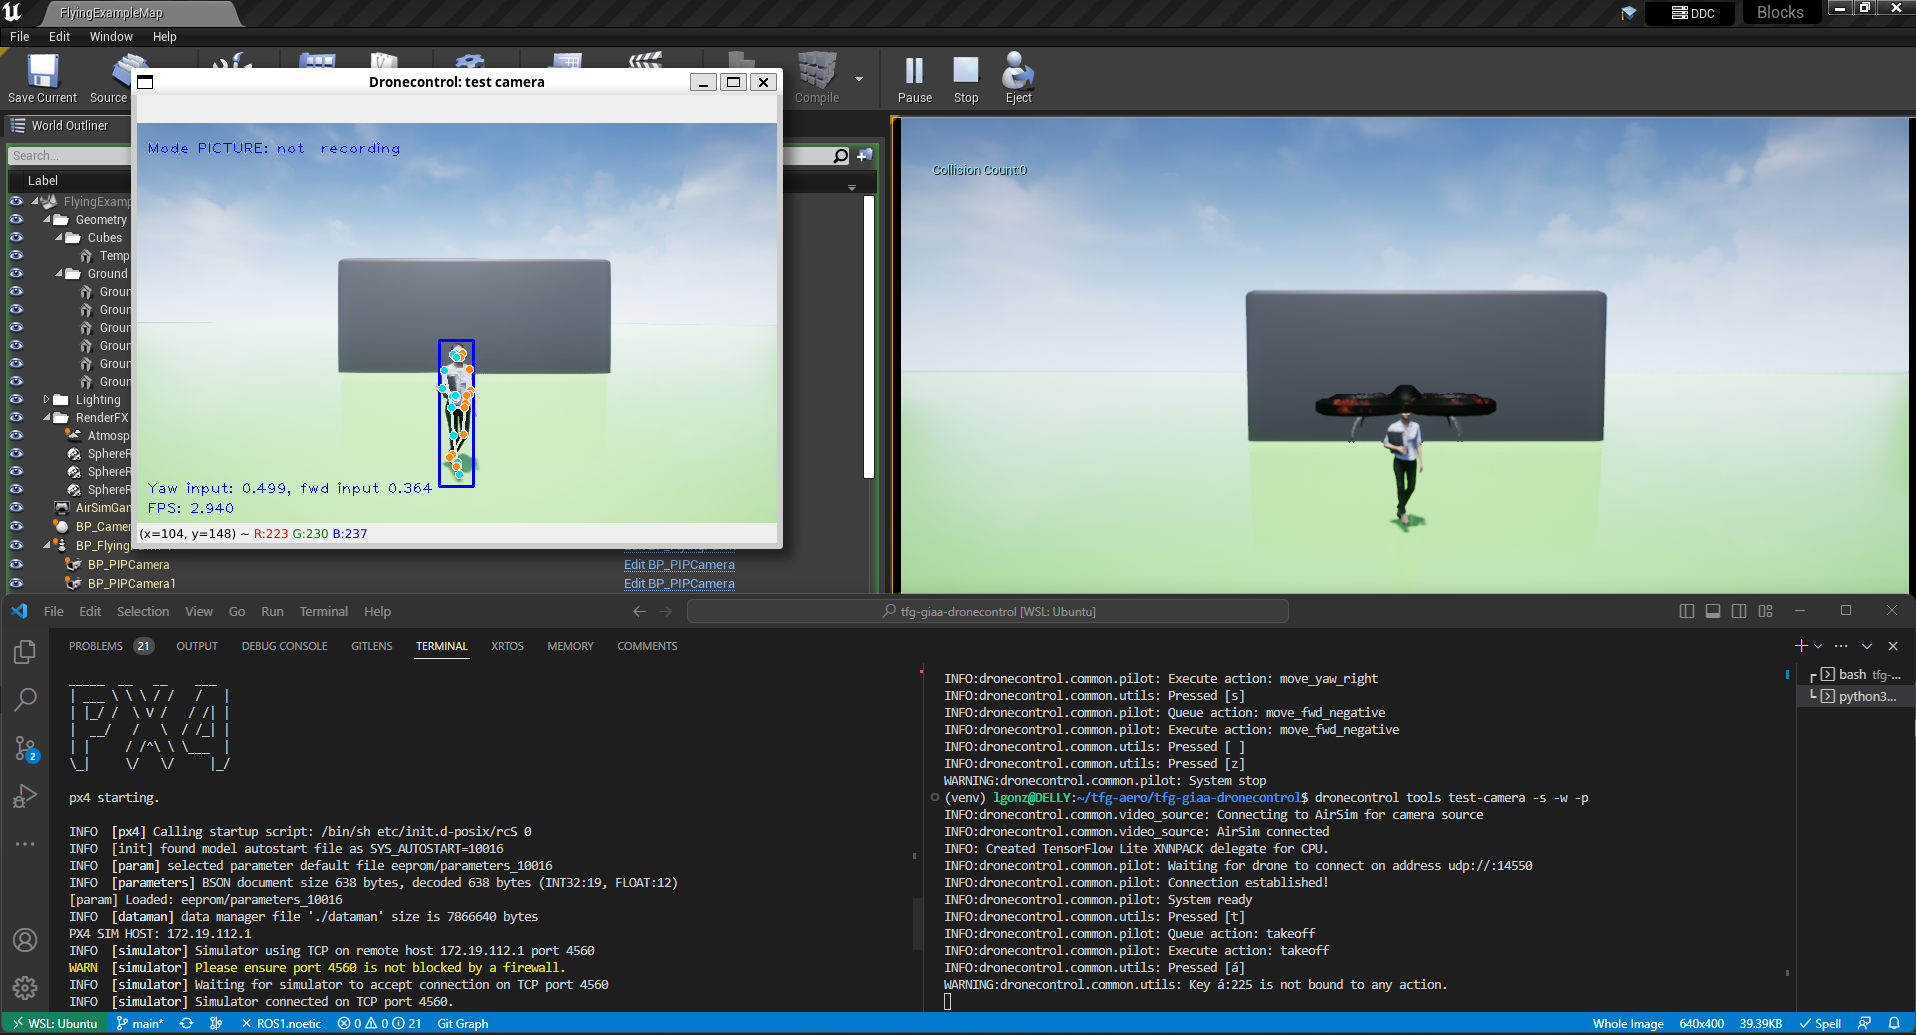
\includegraphics[width=\textwidth, keepaspectratio]{img/airsim-sitl-pose.png}
  \caption{AirSim, PX4 and DroneVisionControl applications running side-by-side and connecting to each other}
  \label{fig:airsim-sitl-pose}
\end{figure}

Now that the testing environment is working as expected and before it is used to tune the PID controllers in the follow solution to the response of the vehicle's movement in the next section, it is possible to verify that the controllers are capable of reacting to changes in the position of the figure by only enabling their proportional term with an appropriately low magnitude to keep the movement slow and smooth.
The drone movement when running the follow control program with values of 10 and 2 on the proportional term of the yaw and forward controllers, respectively, which can be done with the command \mintinline{bash}{dronevisioncontrol follow --sim --yaw-pid (10, 0, 0) --fwd-pid (2, 0, 0)}, is shown in this \href{https://l-gonz.github.io/tfg-giaa-dronecontrol/videos/test-sitl-follow}{video}\footnote{\url{https://l-gonz.github.io/tfg-giaa-dronecontrol/videos/test-sitl-follow}} and a frame extracted from it can be seen in figure \ref{fig:airsim-test-follow}.
\todo[inline]{Match text to video}

\begin{figure}
  \centering
  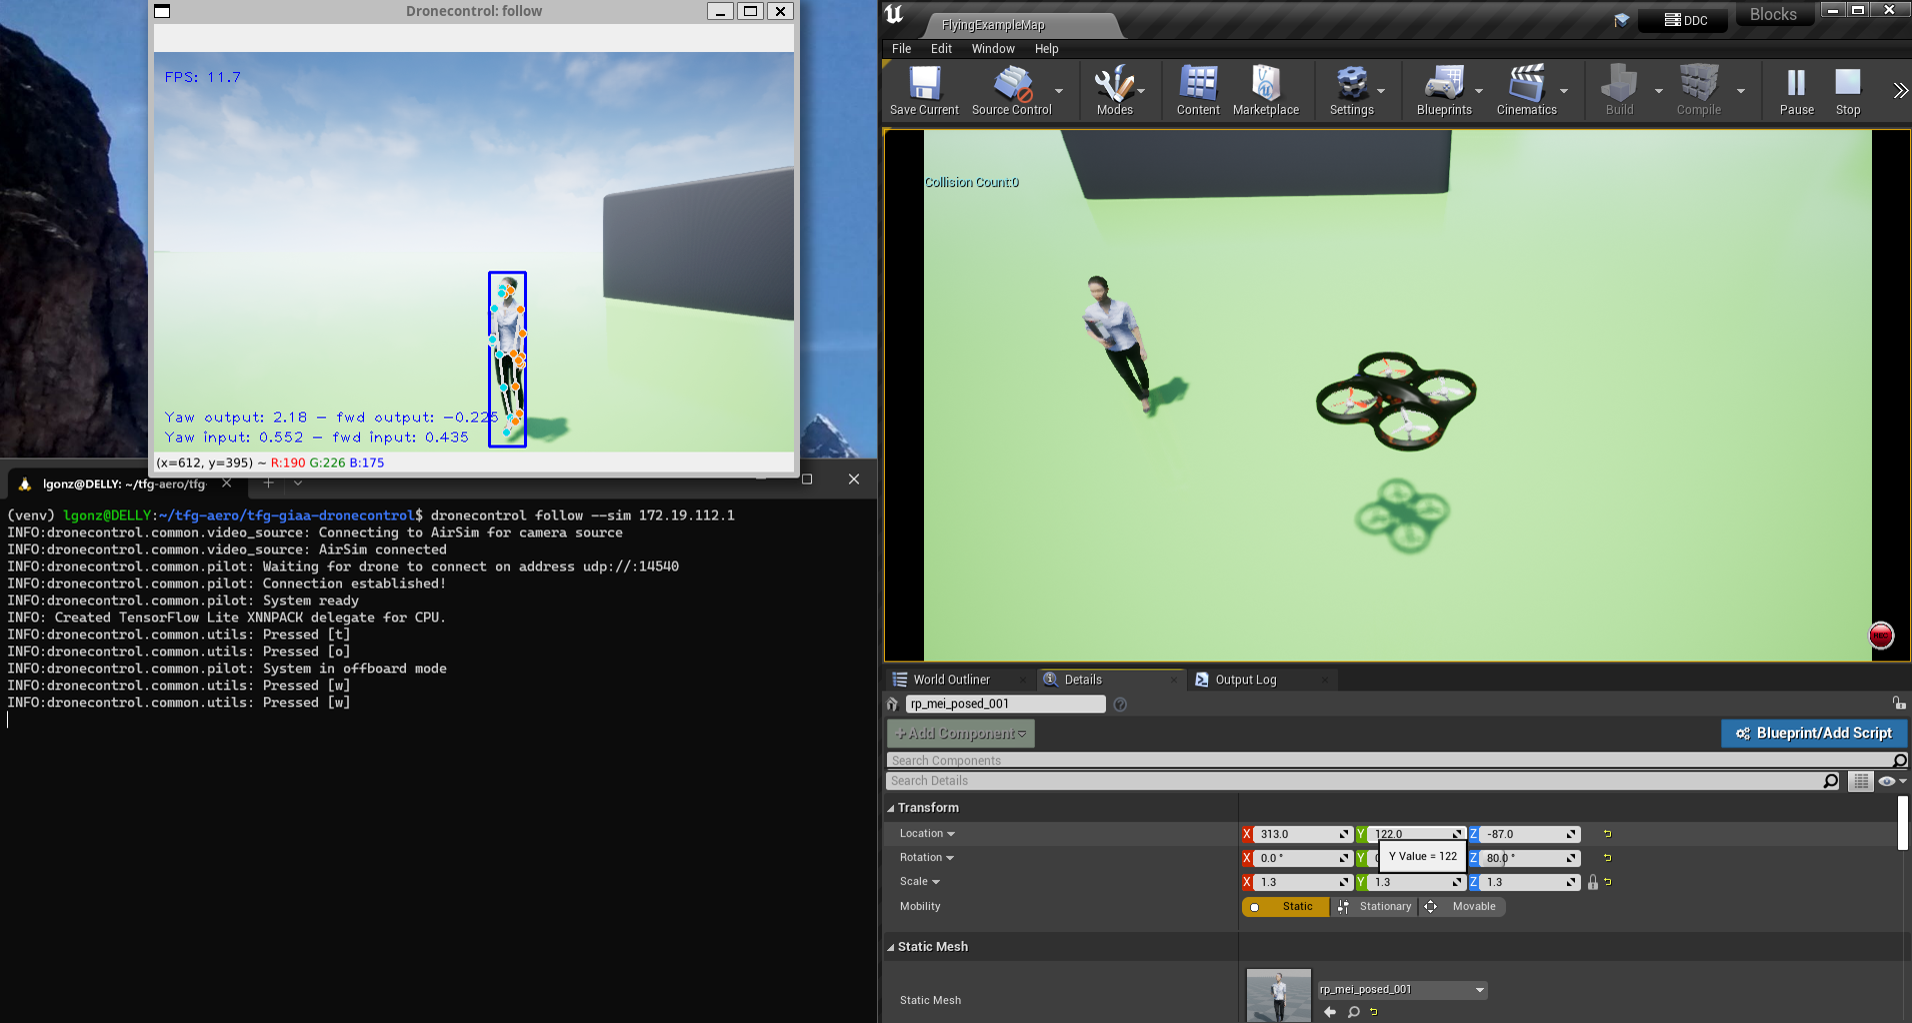
\includegraphics[width=\textwidth, keepaspectratio]{img/video-follow-sitl.png}
  \caption{Single frame from the video showing the movement of the drone in response to changes in the position of the tracked person}
  \label{fig:airsim-test-follow}
\end{figure}

\section{PID controller validation}
\label{sec:test-1-pid}

% Process of tuning the PIDs
% Graphs from test-controller
% Analysis of error

As mentioned before, the velocity controller that is the heart of the person following mechanism is based on two PID controllers.
In order to get velocity outputs for the PID controllers that produce a stable movement of the vehicle, it is necessary to tune the parameters of the controllers until the appropriate combination is found.
In this section, the value for the coefficients used for the project will be found empirically with the help of the tuning tool described in section \ref{subsec:pid-tools} and developed for this purpose. Its performance will be validated with the controller testing tool, both running in the simulated environment with the flight stack in SITL mode so that it is possible to take continuous measures of the response of the PID controllers to step movements of a simulated person present in the 3D world.
In the first place, each controller will be tuned independently of the other by allowing the vehicle only one direction of movement at a time.
Afterwards, both controllers are engaged simultaneously to measure the joint response to a range of different inputs.

The controllers are calibrated for a reference position of x=0, y=0 for the vehicle and x=600, y=0 for the person in world coordinates of the simulated environment.
At these positions, processed images taken from the simulated camera detect the person centred in the field of view and with a height of 36\% of the image height.
This means that the controllers running in the simulator will have as their target set points 0.5 for the yaw controller and 0.36 for the forward controller. 
So for any changes in the position of the simulated person, the controllers will send velocity commands to the autopilot to achieve the same relative position between the vehicle and the person as in the reference shown in figure \ref{fig:tune-start-pos}.

\begin{figure}
  \centering
  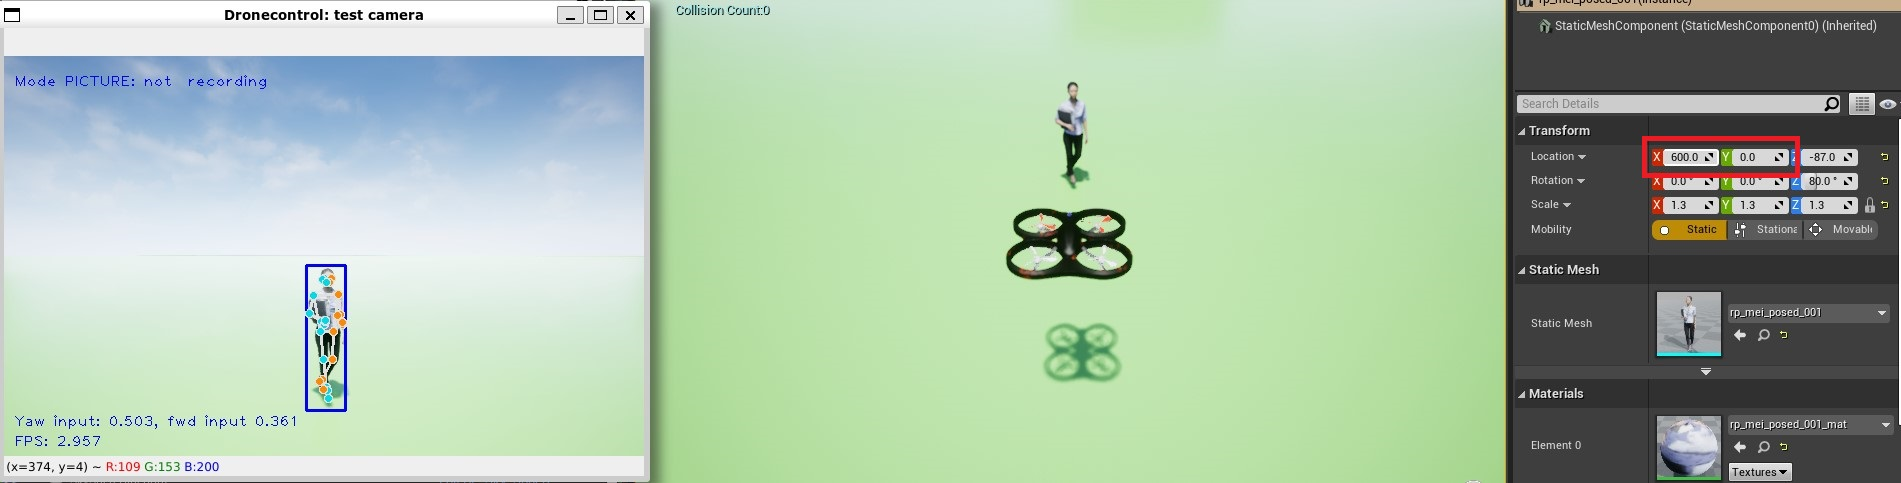
\includegraphics[width=\textwidth, keepaspectratio]{img/pid/tune-ref-pos.jpg}
  \caption{Reference position for the yaw and forward PID controllers. From left to right, the panels show the DroneVisionControl application window, the AirSim simulator world view and the world location of the human model in the simulator. The distance between the vehicle and the person is 600 units in the x direction and 0 units in the y direction.}
  \label{fig:tune-start-pos}
\end{figure}


\subsection{Yaw controller}

\begin{figure}
  \centering
  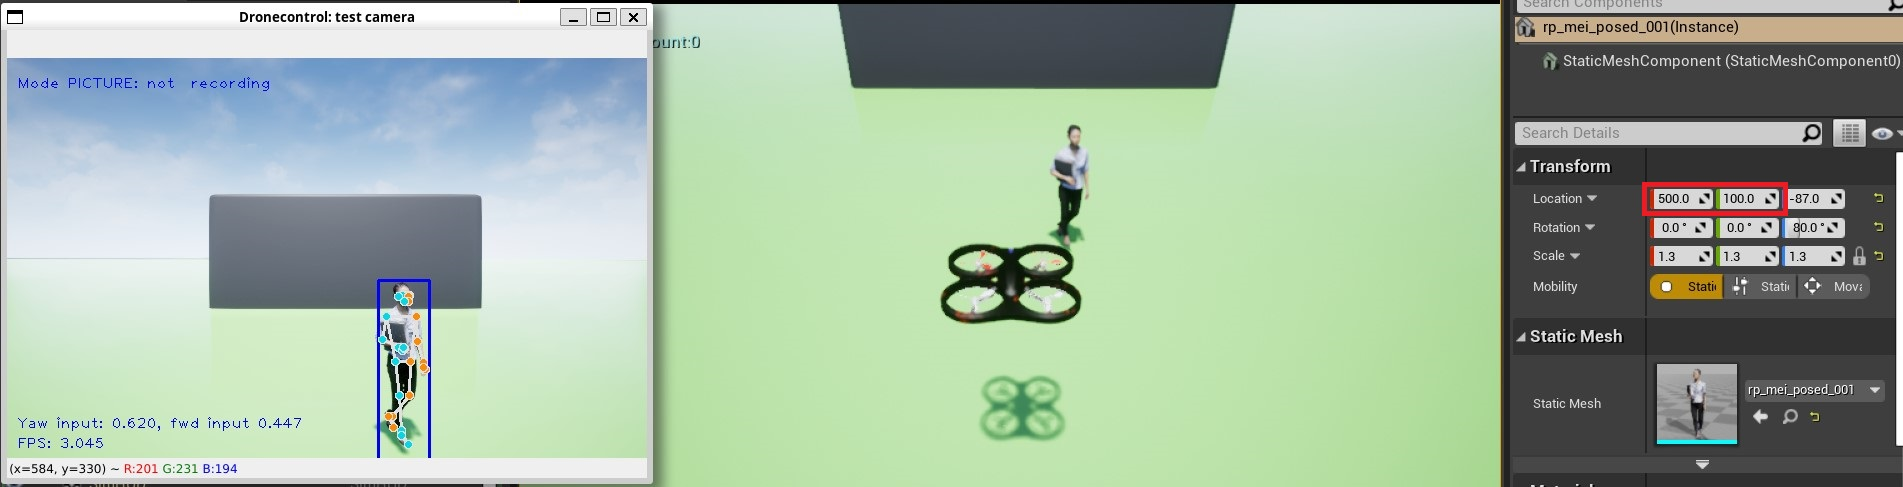
\includegraphics[width=\textwidth, keepaspectratio]{img/pid/tune-ref-pos-yaw.jpg}
  \caption{Starting position of the simulator for tuning the yaw controller. The human model is situated 500 units forward and 100 units to the right of the vehicle model.}
  \label{fig:tune-ref-pos-yaw}
\end{figure}

To find the correct coefficients for the controller that governs the yaw velocity of the vehicle, the target person is set in a position slightly to the side on its field of view so that when the controller is engaged, it outputs a rotation of the vehicle to that side.
Since the forward controller will not be engaged during the test, the target person can be situated closer to the camera to make it easier for the pose detection algorithm to output correct landmarks.
Figure \ref{fig:tune-ref-pos-yaw} shows the starting position of the simulated environment before each run, where the 3D model has been situated at (500, 100), that is, 100 units to the right of the reference position.
On the left-most panel of figure \ref{fig:tune-ref-pos-yaw}, the DroneVisionControl application shows that the input to the yaw controller is 0.62 at this position.
The controller must then output a positive yaw velocity to centre the person in its field of view. 
This offset position to the right produces an error that is less than zero (set point minus input, $\epsilon = 0.5 - 0.62$ ).
However, it requires a positive velocity to counteract and induce a yaw velocity to the right, so the coefficients for the yaw controller will need to be negative so that an increased horizontal position results in a positive yaw velocity to decrease it, as indicated by equation \ref{eq:pid}.
 

\begin{figure}
  \centering
  \makebox[\textwidth][c]{
  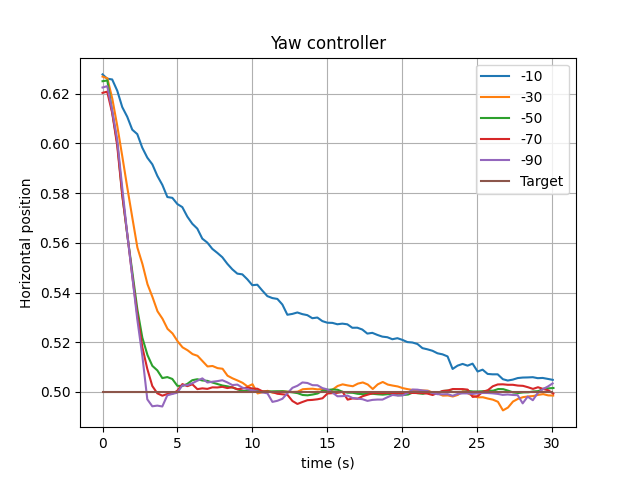
\includegraphics[width=.52\textwidth]{img/pid/yaw/yaw_pos_prop_i0_d0.png}
  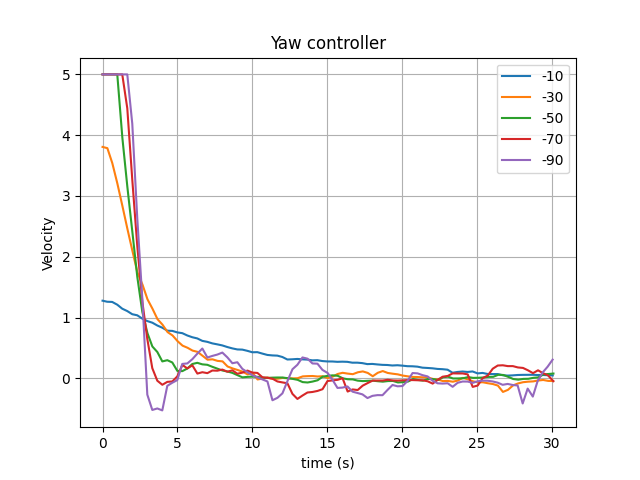
\includegraphics[width=.52\textwidth]{img/pid/yaw/yaw_vel_prop_i0_d0.png}}
  \caption{Variation of (a) input position and (b) output velocity for different values of $K_{P}$ and $K_I=0$, $K_D=0$ while the yaw controller is engaged.}\label{fig:tune-yaw-prop}
\end{figure}

To tune the controller to its correct coefficients, the first step will be to test different values of $K_{P}$ while maintaining $K_{I}$ and $K_{D}$ at zero.
Figure \ref{fig:tune-yaw-prop} shows the output of the tuning program for the five values of $K_{P}$ tested, from $K_P=-10$ to $K_P=-90$ in increments of 20.
The left graph represents the variation of the horizontal position detected by the camera for the first 30 seconds after activating the controller.
The right graph shows the yaw velocity that the controller outputs to the pilot module to reach the target.
For low values of $K_{P}$, the controller makes the vehicle move slowly towards its target so that it takes a long time to reach the midpoint position.
On the other hand, for high values of $K_{P}$, the controller tries to reach the target too fast, so when it gets close to it, it starts to oscillate around the target.
The right side graph also shows well how the output velocity in the yaw controller is limited to 5 degrees per second, so even for very high values of $K_P$, the vehicle will not rotate faster than that.
From the graphs, the best of the values tested is $K_{P}=50$, where the distance to the target point decreases rapidly (left graph), but the velocity does not start to increase and decrease widely around 0 (right graph).

The second step is to find the correct value for $K_I$. 
To do that, several values of $K_I$ will be tested for a low $K_P$ of -20 and $K_D=0$ so that the effect of the integral part is easier to appreciate. Figure \ref{fig:tune-yaw-int-20} shows the evolution of the input and output at the controller for a sample time of 40 seconds for each of the values tested. 
For a low $K_I=-1$, the progress toward the target is stable and slightly faster than without any contribution of the integral part.
However, when the $K_I$ increases in magnitude, it creates initial oscillations around the target position that fade out as time progresses. For a very large $K_I$ from around -10, the vehicle's velocity becomes locally unstable with many slight variations in its oscillations.

\begin{figure}
  \centering
  \makebox[\textwidth][c]{
  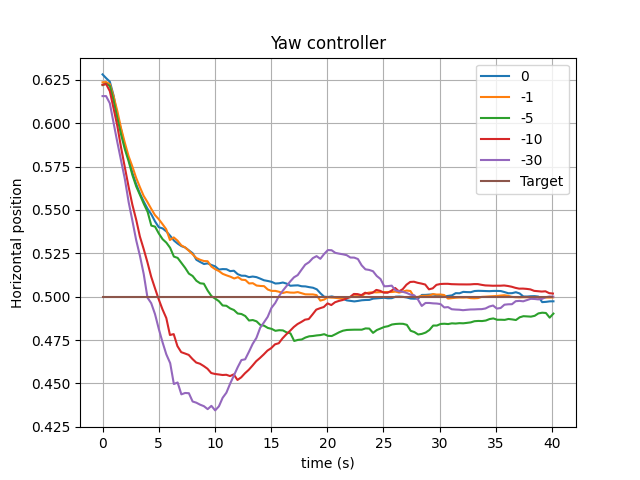
\includegraphics[width=.52\linewidth]{img/pid/yaw/yaw_pos_p20_int_d0.png}
  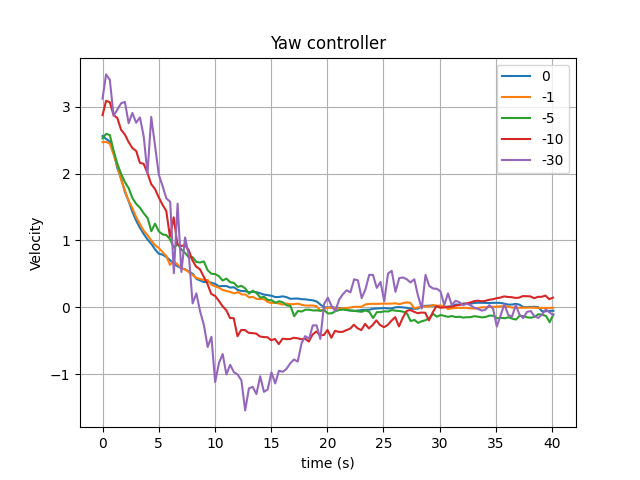
\includegraphics[width=.52\linewidth]{img/pid/yaw/yaw_vel_p20_int_d0.png}}
  \caption{Variation of (a) input position and (b) output velocity for different values of $K_{I}$ and $K_P=-20$, $K_D=0$ while the yaw controller is engaged.}\label{fig:tune-yaw-int-20}
\end{figure}

A similar effect can be observed to a lower extent in figure \ref{fig:tune-yaw-int-50}, where the measurements have been taken for $K_P=-50$ and $K_D=0$. 
In this graph, $K_I=-1$ makes the controller reach the target position some 3 seconds faster and with similar oscillations in its velocity than with the proportional part exclusively ($K_P=-50$, $K_I=0$, $K_D=0$).

\begin{figure}
  \centering
  \makebox[\textwidth][c]{
  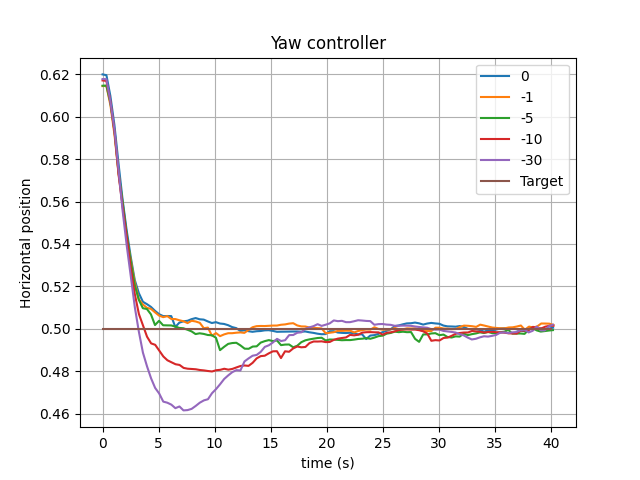
\includegraphics[width=.52\linewidth]{img/pid/yaw/yaw_pos_p50_int_d0.png}
  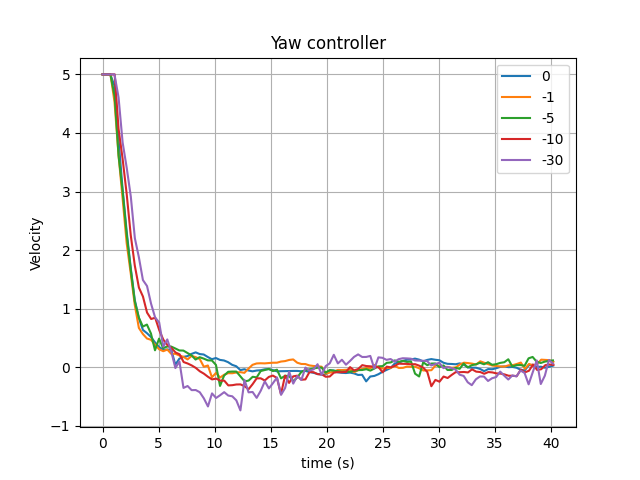
\includegraphics[width=.52\linewidth]{img/pid/yaw/yaw_vel_p50_int_d0.png}}
  \caption{Variation of (a) input position and (b) output velocity for different values of $K_{I}$ and $K_P=-50$, $K_D=0$ while the yaw controller is engaged.}\label{fig:tune-yaw-int-50}
\end{figure}

In the last step, the tuning process will deal with the derivative part of the controller.
In this case, several values of $K_D$ have been tested against the chosen $K_P=-50$, both without any integral part and with $K_I=-1$.
This will allow seeing the effect that the derivative part has in the controller, as well as validating if the integral part chosen in the last step can work together with the derivative part to make the controller react better to a changed input.
Figures \ref{fig:tune-yaw-der-i0} and \ref{fig:tune-yaw-der-i1} show the evolution of the position detected by the computer vision system and the velocity the controller outputs for a sample time of 40 seconds for $K_I=0$ and $K_I=-1$, respectively, with $K_P=-50$.
For all the tested values, the iteration with $K_I=-1$ on \ref{fig:tune-yaw-der-i1} shows a better convergence towards the target positions than their counterpart values of $K_D$ for $K_I=0$, which indicates that the integral part has been chosen correctly.
Furthermore, adding any amount to the derivative part does not produce any visible benefit in the step response of the controller and the curve that first stabilises on the target position continues to be the one for $K_D=0$, while the velocity graph remains approximately the same between $K_D=0$ and $K_D=-2$
The final values for the coefficients for the yaw controller will then be $K_P=-50$, $K_I=-1$, and $K_D=0$, so the controller will, in truth, only be a PI controller and not a complete PID controller.


\begin{figure}
  \centering
  \makebox[\textwidth][c]{
  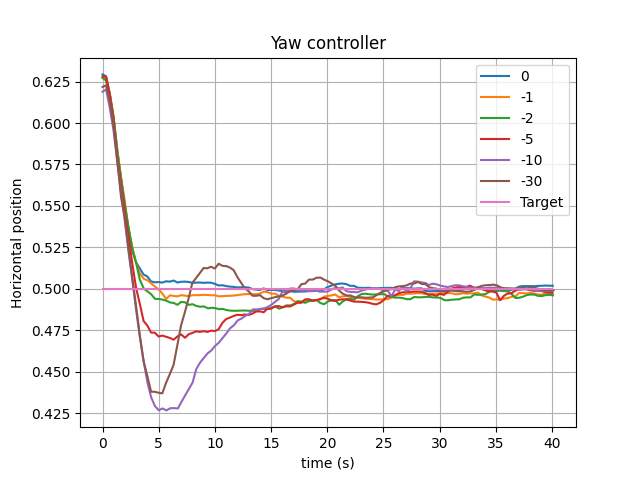
\includegraphics[width=.52\linewidth]{img/pid/yaw/yaw_pos_p50_i0_der.png}
  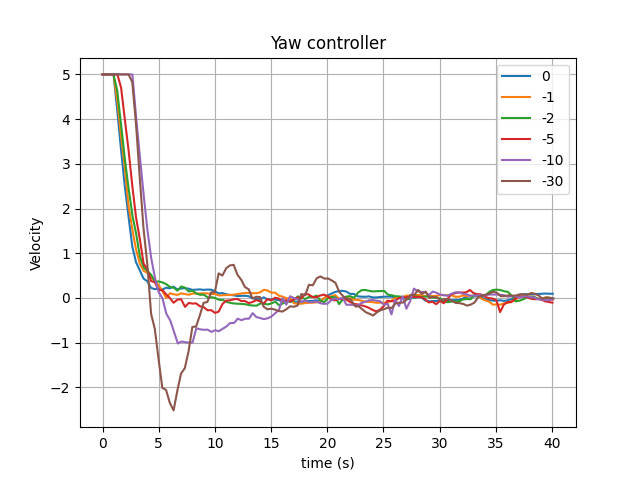
\includegraphics[width=.52\linewidth]{img/pid/yaw/yaw_vel_p50_i0_der.png}}
  \caption{Variation of (a) input position and (b) output velocity for different values of $K_{D}$ and $K_P=-50$, $K_I=0$ while the yaw controller is engaged.}\label{fig:tune-yaw-der-i0}
\end{figure}

\begin{figure}
  \centering
  \makebox[\textwidth][c]{
  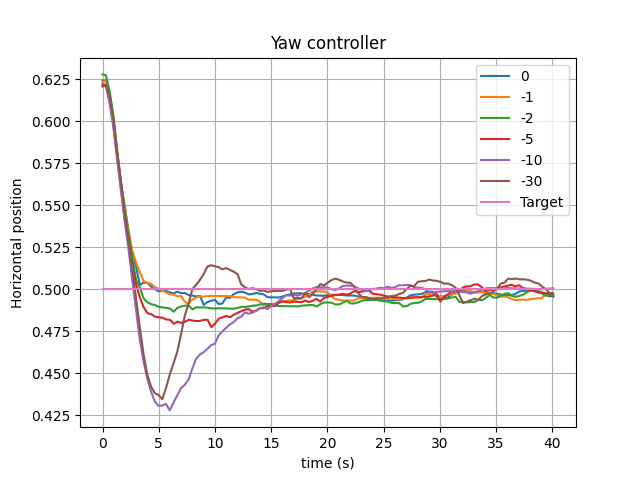
\includegraphics[width=.52\linewidth]{img/pid/yaw/yaw_pos_p50_i1_der.png}
  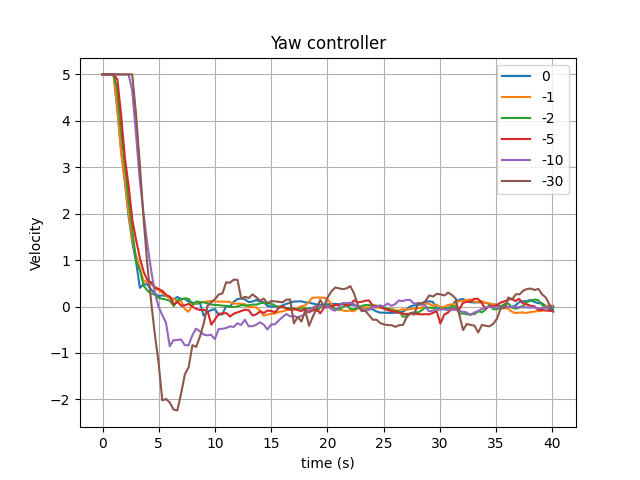
\includegraphics[width=.52\linewidth]{img/pid/yaw/yaw_vel_p50_i1_der.png}}
  \caption{Variation of (a) input position and (b) output velocity for different values of $K_{D}$ and $K_P=-50$, $K_I=-1$ while the yaw controller is engaged.}\label{fig:tune-yaw-der-i1}
\end{figure}

A recording of the whole tuning process for the yaw controller can be seen in this \href{https://l-gonz.github.io/tfg-giaa-dronecontrol/videos/tune-yaw-controller}{video}\footnote{\url{https://l-gonz.github.io/tfg-giaa-dronecontrol/videos/tune-yaw-controller}}.


\subsection{Forward controller}


A similar process to the one used for the yaw controller must be followed for the forward controller.
The starting position for the tuning process is, in this case, with the figure closer to the vehicle than the reference position and centred in its field of view.
Figure \ref{fig:tune-ref-pos-fwd} shows this starting setup with the figure situated at the (450,0) position in the simulated world.
In this position, the input to the forward controller is 0.47, that is, the bounding box around the detected figure takes up 47\% of the height of the camera field of view.
The response from the controller will therefore need to be a negative forward velocity that brings the vehicle away from the target person to reduce the perceived figure height.
Since a negative output velocity reduces the input at the entrance of the controller in a directly proportional manner, the coefficients for this PID controller will need to be positive, contrary to what happened on the yaw controller where the feedback loop was inversely proportional (a positive velocity decreased the input to the yaw controller).


\begin{figure}
  \centering
  \includegraphics[width=\textwidth, keepaspectratio]{img/pid/tune-ref-pos-fwd.jpg}
  \caption{Starting position of the simulator for tuning the forward controller. The human model is situated 450 units forward and centred from the vehicle position.}\label{fig:tune-ref-pos-fwd}
\end{figure}

In general, the forward velocity will always need to be smaller than the yaw velocity since it induces a pitch angle in the vehicle that tilts the camera up and down, which can destabilise the camera and cause a loss of sight of the followed figure.
To achieve that, the coefficients for the forward controller will be reduced by one order of magnitude.
First, values from $K_P=1$ to $K_P=9$ in increments of 2 have been tested for $K_I=0$ and $K_D=0$ for a sample time of 30 seconds.
The curves described by the controller for these coefficients are shown in figure \ref{fig:tune-fwd-prop}.
Compared with the trajectory described by the yaw controller, the forward controller is generally more unstable since fast forward and backwards movements affect the pose detection algorithm.
This is particularly visible at the start of each test as slightly different heights are detected in the image from the camera even though the vehicle is in the same position with respect to the human figure.
It also creates an effect, especially for the bigger $K_P$ values tested, where, as the vehicle begins its movement back to its target position, the pose detection mechanism gets a slightly different perspective on the followed person, which increases the detected height slightly so that small spikes of detected differences show in the height graphs even though the velocity graph shows that the vehicle's direction of movement remains the same.
This effect is reduced by keeping the output forward velocity small in the controller.
In the right graph of figure \ref{fig:tune-fwd-prop}, it is also visible for high values of $K_P$ how the output velocity increases enough that the maximum velocity limit is reached on the forward controller and the output is capped to \unitfrac[0.4]{m}{s}.
For a value up to $K_P=3$, the trajectory described descends rapidly without ending in significant oscillations around the target height, so it is a fair value to keep for the final controller.


\begin{figure}
  \centering
  \makebox[\textwidth][c]{
  \includegraphics[width=.52\linewidth]{img/pid/fwd/aaa_fwd_pos_prop_i0_d0.png}
  \includegraphics[width=.52\linewidth]{img/pid/fwd/aaa_fwd_vel_prop_i0_d0.png}}
  \caption{Variation of (a) input height and (b) output velocity for different values of $K_{P}$ and $K_I=0$, $K_D=0$ while the forward controller is engaged.}\label{fig:tune-fwd-prop}
\end{figure}


The respective tests for $K_I$ and $K_D$ in the forward controller are shown in figures \ref{fig:tune-fwd-int} and \ref{fig:tune-fwd-der}.
Increasing the coefficient for the integral part causes the controller to overshoot the target initially but then stabilise before starting to approximate to the target position.
Since, for this application, overshooting is not desirable, as it can cause safety issues, the chosen value of $K_I$ will be 0.
For the derivative part, every value of $K_D$ tested increases the system's oscillations, so it will also be left out of the forward controller.
The final values for the coefficients for the forward controller will then be $K_P=3$, $K_I=0$, and $K_D=0$, which makes it only a proportional controller.


\begin{figure}
  \centering
  \makebox[\textwidth][c]{
  \includegraphics[width=.52\linewidth]{img/pid/fwd/aaa_fwd_pos_p3_int_d0.png}
  \includegraphics[width=.52\linewidth]{img/pid/fwd/aaa_fwd_vel_p3_int_d0.png}}
  \caption{Variation of (a) input height and (b) output velocity for different values of $K_{I}$ and $K_P=7$, $K_D=0$ while the forward controller is engaged.}\label{fig:tune-fwd-int}
\end{figure}
\begin{figure}
  \centering
  \makebox[\textwidth][c]{
  \includegraphics[width=.52\linewidth]{img/pid/fwd/aaa_fwd_pos_p3_i0_der.png}
  \includegraphics[width=.52\linewidth]{img/pid/fwd/aaa_fwd_vel_p3_i0_der.png}}
  \caption{Variation of (a) input height and (b) output velocity for different values of $K_{D}$ and $K_P=7$, $K_I=0.5$ while the forward controller is engaged.}\label{fig:tune-fwd-der}
\end{figure}


\subsection{PID tuning validation}
\label{subsec:pid-test-controller}

As a final validation for the tuning obtained previously, the \texttt{test-controller} tool described in section \ref{subsec:pid-tools} will be used to check the step response of the controllers to different starting distances for the same coefficients.
Additionally, for this test, both controllers will be engaged simultaneously to verify that they work well together.
Firstly, the positions will vary on the y-axis, that is, the figure will move from left to right in the field of view of the vehicle.
The values for the y coordinate to be tested will be between -150 and 150 units in increments of 50.
The x coordinate of the figure in the simulated world will remain at $x=500$.

Plots of the changes in normalised horizontal distance and normalised figure height detected by the person recognition algorithm during the time the vehicle takes to reach the target distance from the human figure for each of the tested positions can be seen in figure \ref{fig:validate-yaw}.
It is considered that the vehicle has reached its target when the error is less than 2\%, and the output speed at the controller is less than 10\% of the maximum value.
Furthermore, the whole testing process followed with the developed \texttt{test-controller} tool can be seen in this \href{https://l-gonz.github.io/tfg-giaa-dronecontrol/videos/test-yaw-controller}{video}\footnote{\url{https://l-gonz.github.io/tfg-giaa-dronecontrol/videos/test-yaw-controller}}.

Since each starting position differs in distance and orientation to the target, both controllers must be engaged to reach the centre.
The yaw controller then introduces a negative yaw velocity when the figure is on the left half of the camera's field of view and a positive yaw velocity when the figure is on the right half to reach the target horizontal distance of 0.5 (figure centred in the image received from the camera);
Moreover, the forward controller outputs a negative forward velocity to reduce the detected height of the figure from around 0.44 to the target 0.36 since the figure is 100 units closer to the vehicle than the reference position $x=600$.

Figure \ref{fig:validate-yaw}a shows that the most time is spent on starting the movement towards the target and, after that, there is not much difference between the time it takes to reach the -50 position and reaching the -150 position, with the former taking 3 seconds and the later taking around 3.6 seconds.
In figure \ref{fig:validate-yaw}b, all of the trajectories have a very similar graph since the starting distance to the target is practically the same, where the controller makes the vehicle pull backwards so the figure stays far enough, making the detected height decrease.
For the $y=100$ starting position, the initial detected height is very small in the beginning until it reaches the starting point of the other tests.
This occurred because the detection algorithm took longer than usual to identify the person in this particular test.
However, after less than half a second, the detection was stabilised without affecting much the time it took to reach the target or its final position, showing that the controllers can recover from errors in the detection mechanism without affecting the vehicle's movement.


\begin{figure}
  \centering
  \makebox[\textwidth][c]{
  \includegraphics[width=.52\linewidth]{img/pid/validation_yaw.png}
  \includegraphics[width=.52\linewidth]{img/pid/validation_yaw_2.png}}
  \caption{Changes over time in detected horizontal position and height as input for the controllers with different starting positions in the y-axis}
  \label{fig:validate-yaw}
\end{figure}

Additionally, the \texttt{test-controller} tool can be run with varying positions in the x-axis, which means that the tests are run with the human figure at different distances closer and further away from the vehicle while maintaining it in the centre of its field of view (y position will remain 0 for the whole process).
Therefore, the yaw controller will not need to be considered for this test.
The changes over time in the input into the forward controller between each starting position and the target position are shown in figure \ref{fig:validate-fwd}.
The figure reflects a significant difference in how the controller reacts to positions closer than the target distance or further from it.
When the person is very close to the vehicle, there are major differences between detected heights, so the vehicle moves fast away from its position.
However, when the person is further away from the vehicle than the target, large differences in distance are associated with minor differences in detected height, which causes the controller to determine a smaller velocity increase than for the same distance difference if the person was closer to the vehicle.
Therefore it will take a longer amount of time for the vehicle to reach the target.
It is worth noting that even when the person is so close to the vehicle that part of it falls outside of its field of view ($x=300$ in the figure), the pose detection works well enough to interpret where the person should continue outside of the image so that it is still possible for the controller to decide the correct direction of movement.

\begin{figure}
  \centering
  \includegraphics[width=.7\textwidth, keepaspectratio]{img/pid/validation_fwd.png}
  \caption{Changes over time in detected height as input for the forward controller with different starting positions in the x-axis}
  \label{fig:validate-fwd}
\end{figure}

\section{PX4 HITL simulation and validation}
\label{sec:test-4-hitl}

% Setup:    build drone, HITL configuration
% Test:     - AirSim + follow on Windows + Pixhawk
%           - QGroundControl (without program running)
%           - PX4 to computer connection
%           - RC on AirSim
% Results:  images of wiring computer-Pixhawk

The aim of this section is to validate the transition from using a simulated version of the flight stack running on Linux (PX4's software-in-the-loop simulation) to using a physical Pixhawk board with simulated input and output to test the flight controller interaction with the developed program.
To do so, the aim is to be able to run the follow solution to send control commands through the Pixhawk board and observe the movement of the vehicle in the AirSim simulator in the same manner as in the previous section.


QGroundControl contains a specific quadcopter HITL airframe configuration that sets up the board with all the required parameters to activate this new hardware-in-the-loop mode.
It automatically detects the Pixhawk 4 board when connected to the computer through its Micro-USB port.
It is also required to make changes to the AirSim configuration for the simulator to work with HITL mode, namely, activating the option to accept connections through serial.
To test the complete system configuration for HITL described in section \ref{sec:devenv} and outlined in figure \ref{fig:hitl-connections}, the Pixhawk board needs an additional channel of communication to the computer dedicated to the Mavlink exchange with the DroneVisionControl application.
The board will therefore have both a direct cable connection to the computer and a telemetry radio on its \texttt{TELEM1} port with a wireless link to its counterparty radio connected to the computer.
Since the AirSim simulator requires a higher update rate than the DroneVisionControl application, it will employ the faster, cabled link.
The simulator can automatically connect to the board when it is started once the \texttt{UseSerial} option in the AirSim settings is set to true.
The DroneVisionControl program will connect through the telemetry radio by specifying the serial port and corresponding baudrate when launching the application.
Since the flight stack is now running on a physical controller, it is possible to add an RC antenna to the \texttt{PPM RC} port of the board to be able to fly the vehicle with a remote control unit after it has been bound to the receiver\footnote{\url{https://docs.px4.io/main/en/config/radio.html}}.
By configuring one of the switches in the RC unit to change to PX4's offboard flight mode, additional checks to the safety measures of interrupting autonomous flight on flight mode changes or loss of signal from the RC controller can be carried out.
Figure \ref{fig:hitl-setup-picture} shows all the connections mentioned.

\begin{figure}
  \centering
  \includegraphics[width=\textwidth, keepaspectratio]{img/hitl-setup-picture.jpg}
  \caption{Pixhawk 4 board connected to the Raspberry Pi running the DroneVisionControl application and the Windows computer running the AirSim simulator, with telemetry radio for QGroundControl and RC receiver for manual control}
  \label{fig:hitl-setup-picture}
\end{figure}

After all the necessary connections are set up, the program can be started with the following command:
\mintinline{bash}{python -m dronevisioncontrol follow --sim --serial COM[X]:57600}, where the exact COM port will vary depending on the particular USB port to which the telemetry radio is connected.


\subsection{PX4 HITL validation with Raspberry Pi}
\label{sec:test-5-rpi}

% Setup:    Raspberry Pi installation, RPi-Pixhawk connection
% Test:     - AirSim + follow on RPi + Pixhawk
%           - Serial connection
% Results:  wiring, performance metrics

The next step in the transition from a fully simulated environment to real flight is to connect the future onboard computer, the Raspberry Pi 4, to the Pixhawk flight controller and proceed with more realistic tests on the exact hardware that will be controlling the drone.
The main characteristics of the Raspberry Pi that have to be ensured to be able to progress further towards autonomous flight are:
\begin{enumerate}
    \item Capacity to function when power is provided from a battery
    \item Stability of serial connection to the Pixhawk board
    \item Ability to run the DroneVisionControl application and all its dependencies
    \item Connection to an external camera
    \item Performance of the computer vision algorithms with reduced processing power
\end{enumerate}

% installation
% xrdp
% battery tests

The complete installation process of all the required libraries and dependencies for the Raspberry Pi is explained in appendix \ref{app:install-dronecontrol-rpi}.
The most convenient method of controlling the small computer is through a remote desktop connection, where the screen contents and mouse and keyboard input are transmitted through a local network.
This way, accessing the Pi's desktop from the ground station computer is possible even during flight.
One option to achieve this is XRDP\footnote{\url{http://xrdp.org/}}, an open-source implementation of a Microsoft Remote Desktop Protocol server compatible with the Raspberry OS.

The first hardware connection to test is the power supply to the Raspberry.
As detailed in section \ref{subsec:onboard}, the selected method for powering the companion computer in the onboard configuration is through a secondary battery.
The connection will be made with a USB to USB-C cable from the battery to the Raspberry Pi.
The intent behind testing the power supply at this point in this process is to verify that it will be suitable for its purpose before it is actually needed to power the computer onboard the vehicle.
This power source must provide enough power to both maintain the processor running at an appropriate speed and provide power to the external camera in turn, which will be attached to the Pi's board and extract power from it.

A similar connector provides a channel for the Mavlink communication between the flight controller and the onboard computer.
In this case, one end of the connector is attached to the \texttt{TELEM2} port in the board and the TX/RX pins are attached to the UART pins on the Raspberry's GPIO header.
For this serial connection to work, both the flight controller and the companion computer need some additional configuration.
The Pixhawk needs to be configured through QGroundControl to enable a secondary Mavlink channel as, by default, only the \texttt{TELEM1} port used by the telemetry radio is configured.
The necessary parameters to modify and their values are collected in table \ref{tab:telem2-params}.
On the Raspberry side, the serial port comes configured to be used as a terminal instead of as a hardware serial port.
This can be fixed through the \texttt{raspi-config} command-line utility with the following steps: Interface options -> Serial Port -> Disable login shell, enable serial port hardware.
After that, the \texttt{/dev/serial0} address can be used to communicate to the device attached to the UART pins at the baudrate configured through QGroundControl.
The \texttt{raspi-config} tool and the connector used between the flight controller and the companion computer are shown in figure \ref{fig:serial-connection}.

\begin{table}[h!]
 \begin{center}
  \begin{tabular}{l|l}
    Parameter name & Value \\ \hline
    MAV\_1\_CONFIG & TELEM2 \\
    SER\_TEL2\_BAUD & 921600 \\
  \end{tabular}
  \caption{PX4 parameters that need to be configured to enable Mavlink communication through the secondary telemetry port}
  \label{tab:telem2-params}
 \end{center}
\end{table}


\begin{figure}
  \centering
  \makebox[\textwidth][c]{
  \includegraphics[width=.615\textwidth, keepaspectratio]{img/raspi-config.png}
  \includegraphics[width=.385\textwidth, keepaspectratio]{img/rpi-pixhawk-serial.jpg}}
  \caption{a) Picture of Raspberry's \texttt{raspi-config} and b) close-up of Pixhawk to Pi cable connection}
  \label{fig:serial-connection}
\end{figure}

The test camera utility will be used to validate this configuration.
At this point, the only physical connection to the ground station running AirSim or QGroundControl is through the development-only micro-USB port in the Pixhawk.
The results from running: \\
\begin{listing}[h!]
    \begin{minted}[breaklines, fontsize=\footnotesize, baselinestretch=1]{bash}
dronevisioncontrol tools test-camera --hardware /dev/serial0:921600 --sim <AirSim host IP> --pose-detection
    \end{minted}
\end{listing}\\
can be seen on figure \ref{fig:rpi-airsim-test}.
On the right side, the remote connection to the Raspberry's desktop shows the output of the DroneVisionControl program running the pose detection algorithm on the images received from the simulator.
On the left side, the AirSim simulator shows the vehicle's movements as it reacts to the input from the flight controller and the companion computer.

\begin{figure}
  \centering
  \includegraphics[width=\textwidth, keepaspectratio]{img/airsim-rpi-test.png}
  \caption{Left: AirSim simulator on Windows host, right: RPi desktop with DroneVisionControl application and pose output}
  \label{fig:rpi-airsim-test}
\end{figure}

\subsection{Performance analysis}
\label{subsec:performance}

The main question left to answer before the vehicle can take to the air with this hardware and software is whether the less powerful processor in the Raspberry Pi 4b, a quad-core ARM Cortex-A72 64-bit SoC running at 1.5GHz, can handle the detection and tracking algorithms with enough performance to get similar results to those obtained with simulated hardware and achieve good reactions to real-time movement.
To do that, the average time that the program spends on each task in the running loop can be calculated and analyzed for different scenarios.
Then it will be possible to estimate the maximum speed at which the person being followed by the algorithm can move.

% Make sure there's a good loop diagram in that section pointed below, and that the enumerated parts are explained in detail
% Match numbers to added figures
From the follow loop presented in section \ref{sec:follow}, it is possible to divide the processing cost into several areas that can be measured independently: image processing, offboard control, manual input, and released thread (sleep).

\begin{figure}
  \centering
  \includegraphics[width=.9\textwidth, keepaspectratio]{img/sitl-performance.png}
  \caption{Average percentages of a loop spent by each task in the follow solution with their corresponding average absolute times in seconds.}
  \label{fig:perf-sitl-sim}
\end{figure}

Figure \ref{fig:perf-sitl-sim} shows the time used for each task on an average run of the follow solution with simulated hardware (PX4 running in SITL mode with AirSim).
The time measurements have been taken by calculating the time difference between each statement's start and end and averaging across every iteration of the main loop.
The main cost in time of each execution is found in the image processing task, which takes around 89\% of the total loop time to run.
This is where the most significant differences in performance will come from between the simulated hardware and the solution running in the Pixhawk 4 + Raspberry Pi combination.
This image analysis process can be further subdivided to get a finer degree of control over how much time each part takes.
The three subtasks that makeup image processing are:
\begin{enumerate}
    \item Get frame: request a new frame from the video source.
    \item Process pose: send the frame to MediaPipe library for detection and tracking.
    \item Detect: calculate bounding box coordinates and define whether it is a valid pose.
\end{enumerate}

This further division is also shown in figure \ref{fig:perf-sitl-sim}, with each of these subtasks taking 40\%, 48\%, and 1\% of the total image processing time, respectively.
The total average time for each run of the follow loop is then 0.094 seconds, which results in an average performance of 10.5 FPS (frames-per-second).

Similar measurements have been taken for hardware combinations with different degrees of simulation, running the follow solution with offboard mode enabled and connected to the AirSim simulator.
These are:
\begin{enumerate}
    \item All simulated hardware: PX4 on SITL mode + DroneVisionControl on standalone computer + images from AirSim simulator video source.
    \item Simulated hardware with real images: PX4 on SITL mode + DroneVisionControl on standalone computer + images from the attached camera as video source.
    \item Test hardware with AC power supply: PX4 on HITL mode on Pixhawk 4 + DroneVisionControl on Raspberry Pi + images from the attached camera as video source.
    \item Test hardware with battery: PX4 on HITL mode on Pixhawk 4 + DroneVisionControl on Raspberry Pi powered by battery + images from the attached camera as video source.
\end{enumerate}


\begin{figure}
  \centering
  \includegraphics[width=\textwidth, keepaspectratio]{img/performance-graph.png}
  \caption{Average FPS and time spent on each task per iteration of the follow solution for the different hardware configurations.}
  \label{fig:perf-analysis}
\end{figure}


Figure \ref{fig:perf-analysis} shows the averages of the measurements taken for all the hardware combinations analyzed.
In the first test, it can be observed that the retrieval of each new frame from the AirSim simulator takes a much longer time than when an external camera is used.
This is because the simulation running on Unreal Engine is also limited in performance to what the computer can offer, which is not a cost that will be reflected when the simulation engine is no longer needed.
In the second test, the images from the simulator are replaced with the feed from an external camera connected to the computer. 
This results in a much lower cost for image retrieval and the best performance of any of the tests, with an average of 14 FPS and peaks of more than 20 FPS.
For the third and fourth tests, the image-processing calculations are moved to the onboard Raspberry Pi computer, which increases the time needed for pose-processing by one order of magnitude.
There is also a noticeable difference in performance in the Raspberry's processor between powering the computer through the AC power supply and through an external battery, stemming from the fact that the former supplies 3A of current to the board and the latter only 2A.

With these measurements, it is possible to understand how the board will behave during actual flight, with the last test being the closest to the expected flight conditions.
It should therefore be possible to sustain a performance of around 3 FPS during flight.
With a time between frames of around 0.3 seconds, and since the field of view of the camera used for flight tests is about four meters wide, the person being followed should be able to move at a speed of 3-4 m/s and remain within the view of the drone.


%% NICE TO HAVE:
%% Keyboard control actor in unreal that can walk around at a set speed
%% and be followed
%% EVEN NICER TO HAVE:
%% Web build of unreal project running dronecontrol


\clearpage
\section{Quadcopter flight tests}

After validating the performance and safety of the control algorithms in the simulated environment, the next step involves conducting flight tests with a fully-built physical UAV. This final phase of the validation process aims to assess the performance of the developed software with all the previously analysed components together in a real quadcopter during flight. To achieve this, first, the base vehicle will be constructed using the chosen development kit. Subsequently, all additional components required for this project, such as the companion computer and camera, will be integrated into the base frame. Once the vehicle can successfully fly with the full payload under remote control, the developed control solutions will be tested.

The initial test will run the hand-control solution to verify that the autopilot can receive flight commands from an offboard computer outside of the simulation. Next, the follow mechanism will be started to confirm that the companion computer can function in flight as well as it did during the simulation tests.

The exact steps that will be executed one after the other to ensure that safety is maintained during the whole process are as follows:
\begin{enumerate}
    \item Assemble the quadcopter with its basic components.
    \item Attach the custom payload.
    \item Conduct a test flight using only the remote control and factory autopilot while monitoring through QGroundControl.
    \item Perform a flight using the custom software from an offboard computer, utilizing the \texttt{test-camera} tool.
    \item Conduct a flight using the \texttt{test-camera} tool from the onboard computer.
    \item Perform a flight using the custom hand-gesture control solution from the offboard computer.
    \item Conduct a flight using the custom follow solution from the onboard computer.
\end{enumerate}


\subsection{Build process}
\label{sec:test-7-builddrone}

The chosen vehicle for this project is the Holybro X500, specifically designed to be compatible with PX4. The PX4 documentation\footnote{\url{https://docs.px4.io/main/en/frames_multicopter/holybro_x500_pixhawk4.html}} provides detailed instructions on how to build the vehicle using its Development Kit. Figure \ref{fig:x500-dev-kit} illustrates all the components required to construct the complete vehicle.

\begin{figure}[H]
  \centering
  \includegraphics[width=.9\textwidth, keepaspectratio]{img/x500-dev-kit.jpg}
  \caption{Development kit for the Holybro X500.}
  \source{Adapted from \citetitle{px4-guide} \cite{px4-guide}.}
  \label{fig:x500-dev-kit}
\end{figure}


Once the standard parts are assembled, the custom additions can be integrated into the remaining space within the frame. The Raspberry Pi companion computer will be positioned between the autopilot and GPS antenna. This placement facilitates a convenient connection between the autopilot and the Raspberry Pi's I/O pins using short cables, preventing excessive wire clutter within the frame. 


During flight, the Raspberry Pi will be powered by a dedicated external battery, which supplies power through a 2-ampere USB port. This port will be connected to the Raspberry Pi's original power cable, utilizing its USB-C power supply socket. As explained in Section \ref{sec:test-5-rpi}, this power supply is sufficient to operate the connected camera and run the developed software with satisfactory performance. The battery will be positioned beneath the autopilot, as depicted in Figure \ref{fig:full-build}. 


\begin{figure}[H]
  \centering
  \includegraphics[width=1\textwidth, keepaspectratio]{img/full-build.jpg}
  \caption{Complete build of the quadcopter with the main components highlighted.}\label{fig:full-build}
\end{figure}


To ensure the camera is securely mounted on the vehicle's frame, the custom-built support system described in Section \ref{subsec:onboard} will be utilized. The camera holder will be attached to the slide bars beneath the main frame, positioning the camera's weight as close to the centre of mass as possible behind the GPS platform. The main battery, responsible for powering the engines and autopilot, and located on the underside of the carbon frame, can be shifted along the forward axis to balance the added weight from the companion computer, its battery and the camera so that the centre of gravity falls approximately in the centre of the vehicle. Figure \ref{fig:camera-holder-closeup} shows the vehicle's underside with the attached camera and the strap for holding the main battery.

\begin{figure}[H]
  \centering
  \includegraphics[width=0.75\textwidth, keepaspectratio]{img/underside-2.jpg}
  \caption{Underside of the vehicle, with the supports for holding the main battery and the camera in place.}
  \label{fig:camera-holder-closeup}
\end{figure}


Once the vehicle construction is complete, additional installation and calibration steps are necessary before it can be flown. These steps, outlined in the build instructions, should include disabling any previously activated simulation modes in the vehicle configuration. Furthermore, the \texttt{MAV\_1\_CONFIG} parameter must be set to \texttt{TELEM2}, as explained in Section \ref{subsec:offboard}. Calibration of all the onboard and externally attached sensors specific to this build is also required. The QGroundControl ground station application provides a configuration screen with the necessary calibration tools for vehicle setup, as depicted in Figure \ref{fig:qgc-config}. The vehicle configuration can be performed either by directly connecting the flight controller to a computer via the micro-USB port or wirelessly by connecting the companion telemetry radio to the computer running QGroundControl.


\begin{figure}[H]
  \centering
  \makebox[\textwidth][c]{
  \includegraphics[width=0.5\textwidth, keepaspectratio]{img/qgc-config-1.png}
  \includegraphics[width=0.5\textwidth, keepaspectratio]{img/qgc-config-3.png}}\\
  \includegraphics[width=0.5\textwidth, keepaspectratio]{img/qgc-config-2.png}
  \caption{Screenshot from the QGroundControl calibration and setup tools used to configure the vehicle.}\label{fig:qgc-config}
\end{figure}


\subsection{Initial tests}
\label{sec:test-8-flight}


\subsubsection{Baseline flight with factory software}
\label{subsec:fl-test-1}

Once the vehicle is fully configured, testing the assisted takeoff and landing can be conducted using the RC controller and QGroundControl. At this stage, the drone should be capable of maintaining stable flight using autopilot-assisted flight modes, such as Position Mode. In Position Mode, the roll and pitch sticks in the controller control the vehicle's acceleration over the ground in the forward/backward and left/right directions, respectively, relative to the vehicle's heading. The throttle stick controls the ascent and descent speed. When the sticks are centred, the vehicle actively maintains its position in 3D space, compensating for wind and external forces. This semi-manual mode can serve as a safe means to verify the functionality of the factory autopilot.


Through QGroundControl, it is possible to map different switches on the RC controller to various autopilot commands. For the test, a two-position switch will be mapped to the armed/disarmed state in order to control the quadcopter's engine startup. A three-position switch will be assigned to change the vehicle's flight mode between the landing, takeoff and position modes. By shifting between the available switch positions during flight, the primary autopilot modes can be tested. Any other flight modes or triggers that need to be used can be set directly through the QGroundControl interface during flight.


To initiate the flight, the main battery is connected to the power module socket. This action powers up the autopilot, GPS antenna, telemetry radio, and RC receiver. Subsequently, QGroundControl is launched on a computer connected to the second telemetry radio via USB. If all connections have been established correctly, the ground station application will automatically connect to the vehicle and display its position on a satellite map. Similarly, turning on the RC controller establishes its connection with the vehicle, provided they have been correctly paired together as outlined in the build instructions guide. Once all wireless connections are established, the drone can take off by switching to the armed state, followed by selecting the takeoff flight mode. While the drone is airborne, switching to the position flight mode enables direct control through the joysticks on the controller.


\subsubsection{Offboard computer flight with test tool}
\label{subsec:fl-test-2}

The second test flight aims to verify that the custom software (DroneVisionControl) can wirelessly transmit takeoff and landing commands from the offboard computer using a MAVlink channel. The channel will be established by taking advantage of the developed \texttt{test-camera} tool through the telemetry radio. During this flight, it is important to note that the QGroundControl application cannot be connected to the vehicle as it will interfere with the telemetry radio channel used by the DroneVisionControl application. Consequently, the RC controller will serve as a backup in case of any issues with the software. The controller can be used to switch flight modes and override inputs from the DroneVisionControl application, providing manual control if necessary.

Since the DroneVisionControl application will arm the vehicle on its own by sending a takeoff command and to ensure safety during flight, the two-way switch on the controller will be mapped on all subsequent tests to the command to cut off power to the engines. This command can be valuable in exceptional situations where it is necessary to protect the vehicle or the surrounding area, such as if the autopilot were to destabilize during takeoff and landing or there was a complete loss of control during flight.

To initiate the test, the main battery is reconnected to the power module. Then, the following command is executed on the offboard computer, depending on whether it is desired to be run on a Windows or Linux machine.


\begin{minted}[escapeinside=||,breaklines,fontsize=\footnotesize, baselinestretch=1]{bash}
|Windows:| dronevisioncontrol tools test-camera --hardware COM<X>:57600
|Linux:| dronevisioncontrol tools test-camera --hardware /dev/ttyUSB0:57600}
\end{minted}


After successfully establishing the connection with the vehicle, the computer keyboard can be used to control the flight. Pressing the T key triggers takeoff, while the L key initiates the landing process. The O key sets the autopilot to offboard flight mode, enabling it to receive velocity commands. Subsequently, the WASD keys will control the forward and sideways movement of the vehicle, and the QE keys will adjust its yaw rotation.

Figure \ref{fig:flight-test-cam-offboard} illustrates the output displayed in the computer's terminal window, showcasing the connection process, the sent velocity commands, and the camera output from the offboard computer. Additionally, a video capturing the entire process can be accessed in the project's href{https://l-gonz.github.io/tfg-giaa-dronecontrol/videos/flight-test-offboard}{website}\footnote{\url{https://l-gonz.github.io/tfg-giaa-dronecontrol/videos/flight-test-offboard}}.

\begin{figure}
  \centering
  \includegraphics[width=\textwidth, keepaspectratio]{img/video-field-test-offboard.png}
  \caption{Terminal output from the \texttt{test-camera} tool running on an offboard computer and image of the drone flying in response.}
  \label{fig:flight-test-cam-offboard}
\end{figure}

\subsubsection{Onboard computer flight with test tool}
\label{subsec:fl-test-3}


The third and final test flight in this section aims to confirm that the custom software can send takeoff and landing commands through a cabled MAVlink channel from the onboard computer. Additionally, it ensures that the onboard camera can capture a clear image of the vehicle's field of view during flight.

For this test, the same tool used in the previous test will be executed on the Raspberry Pi, utilizing the wired serial link between the onboard computer and the Pixhawk autopilot board. As the tool will now use the camera connected to the companion computer, positioned to look down on the pilot, pose detection can be activated on the received images.


To initiate the flight test, the main battery needs to be attached to the power module and the secondary battery to the Raspberry Pi. Once the onboard computer has started, it will be operated through a remote desktop connection via WiFi. Using this connection, a terminal window can be opened on the desktop to execute the following command:
\begin{minted}[breaklines, fontsize=\footnotesize, baselinestretch=1]{bash}
dronevisioncontrol tools test-camera --hardware /dev/serial0:921600 --pose-detection
\end{minted}


Unlike the telemetry radio flight, this test employs a serial connection running at a baud rate of 921600, matching the configured baud rate on the \texttt{TELEM2} port of the Pixhawk board. The \texttt{-p} option enables pose detection in the output images. A video documenting the entire process can be accessed on this \href{https://l-gonz.github.io/tfg-giaa-dronecontrol/videos/flight-test-onboard}{link}\footnote{\url{https://l-gonz.github.io/tfg-giaa-dronecontrol/videos/flight-test-onboard}}. Additionally, an image extracted from the video can be seen in Figure \ref{fig:flight-test-cam-onboard}.


\begin{figure}
  \centering
  \includegraphics[width=\textwidth, keepaspectratio]{img/video-field-test-onboard.png}
  \caption{Pose detection algorithm running on images taken during flight.}
  \label{fig:flight-test-cam-onboard}
\end{figure}


\subsection{Hand gesture control}
\label{subsec:fl-test-4}


During the basic flight tests, all the connections and individual components of the software were validated in realistic flight scenarios. Now, the focus shifts to integrating the piloting system with the results of image recognition to test the developed vision-based control solutions.

The first solution to be tested in flight is the hand-gesture guidance system, which runs on an offboard computer without performance constraints and doesn't rely on battery power. The setup for this test will be the same as the second test flight, described in Section \ref{subsec:fl-test-2}, using the telemetry radio for the serial link and disregarding the onboard companion computer. Once the autopilot board is powered up, the control solution is initiated by executing the following command, where <device> is replaced with the appropriate COM port or TTY device to which the telemetry radio is connected, depending on the platform.
\begin{minted}[breaklines, fontsize=\footnotesize, baselinestretch=1]{bash}
dronevisioncontrol hand --serial <device>:57600
\end{minted}


Once the pilot connection is established, the image from the computer's webcam will be displayed on the screen with an outline highlighting any detected hand. To begin controlling the vehicle, the open palm gesture should be shown to the camera. Closing the hand into a fist will initiate takeoff, and pointing up with the index finger will activate the offboard flight mode. Moving the index finger right or left will cause the vehicle to mirror the movement, while moving the thumb right or left will make the vehicle move forwards and backwards, respectively. At any point during the test, displaying an open hand will cause the drone to hover in its current position. Losing sight of the controlling hand will also trigger the hovering mode.


A video showcasing the entire process can be accessed on this \href{https://l-gonz.github.io/tfg-giaa-dronecontrol/videos/flight-test-hand}{link}\footnote{\url{https://l-gonz.github.io/tfg-giaa-dronecontrol/videos/flight-test-hand}}. Additionally, an image extracted from the video can be seen in Figure \ref{fig:flight-test-hand}.

\begin{figure}[H]
  \centering
  \includegraphics[width=\textwidth, keepaspectratio]{img/video-field-test-hand.png}
  \caption{Image taken during flight controlled by the hand-gesture solution. The vehicle is moving forward.}
  \label{fig:flight-test-hand}
\end{figure}


\subsection{Target detecting, tracking and following}
\label{subsec:fl-test-5}

The last test to conduct is for the follow control solution. In this section, the companion computer will run the follow program with the aim of tracking and following a moving target outside of simulation. The setup for this test will be the same as the third test flight, described in Section \ref{subsec:fl-test-3}. Without the need for a wireless telemetry connection on the DroneVisionControl side, the telemetry radio can be utilized to track the vehicle's path using the QGroundControl application on a secondary offboard computer. The control application will be started with the following command:
\begin{minted}[breaklines, fontsize=\footnotesize, baselinestretch=1]{bash}
dronevisioncontrol follow --serial /dev/serial0:921600
\end{minted}
This \href{https://l-gonz.github.io/tfg-giaa-dronecontrol/videos/flight-test-follow}{video}\footnote{\url{https://l-gonz.github.io/tfg-giaa-dronecontrol/videos/flight-test-follow}} showcases the process of the vehicle taking off (T key) and activating offboard flight mode (O key) to initiate the tracking of a detected figure. Figure \ref{fig:flight-test-follow} presents an image extracted from this video.


\begin{figure}[H]
  \centering
  \includegraphics[width=\textwidth, keepaspectratio]{img/video-field-test-follow.png}
  \caption{Terminal and image output of the DroneVisionControl follow solution running on the Raspberry Pi.}
  \label{fig:flight-test-follow}
\end{figure}


During the flight test, the application running on the Raspberry Pi achieves a maximum frame rate of around 6 FPS when the follow mechanism is active and approximately 8 FPS when it is disabled by switching out of offboard flight mode. In practical terms, this means that the person being tracked by the drone needs to move relatively slowly to ensure that the camera does not lose sight of them before the control loop can send the command to the vehicle to move to the previously detected position. However, for a proof-of-concept scenario, this performance is acceptable.


At the end of the program execution, the average loop time and average runtime for each task in the control loop are displayed in the terminal. Based on the measurements obtained during the test flight, the average frame rate is calculated to be 3.58 FPS. Figure \ref{fig:flight-performance} compares these measurements with those analyzed in Section \ref{subsec:performance}, particularly with the test configuration selected to most closely resemble actual flight conditions (autopilot board running on HITL mode and the companion computer powered by the secondary battery). Very similar results are recorded for both tests, confirming the simulation configuration employed as a valid method of obtaining realistic results without complex or costly flight tests.

Overall, this test flight verifies the effectiveness of the follow control solution and its ability to track and follow a moving target during a real flight scenario, as well as the validity of the simulation process to obtain realistic results.


\begin{figure}
  \centering
  \includegraphics[width=\textwidth, keepaspectratio]{img/perf-hitl-flight.png}
  \caption{Average loop time for each individual task in the follow control solution and total frame rate for realistic simulation versus actual test flights.}
  \label{fig:flight-performance}
\end{figure}


\clearpage

% CONCLUSIONES %
\chapter{Conclusions}
\label{chap:conclusion}

This chapter analyses the results obtained from the project, as well as the obstacles that arose during the development and testing phases.
Afterwards, the proposed initial objectives are examined for completion, and the lessons learned during the project are exposed, along with some suggestions for future work in the field.

\section{Evaluation of objectives}
\label{sec:consecucion-objetivos}

The main objective of this project was to illustrate how the PX4 platform could be used to develop vision-driven control mechanisms for UAVs.
This was achieved by building and presenting a complete development environment that can be used for each stage in the process of creating new control solutions, from the concept phases to running tests in the target hardware.

For the more specific objectives, in the first place,
the tools and systems developed by the Dronecode Project, which includes PX4, MavSDK and QGroundControl, were leveraged in cooperation with the DroneVisionControl written code to reduce the workload of the project by making use of preexisting and stable technologies.

Second, to show the minimum requirements needed to develop an individual control solution, a combination of low-cost and accessible hardware was employed to test all the developed software and take the project out of the simulation environment and into a real drone capable of flying.
Thanks to the platform's modular nature, all the individual pieces are also interchangeable with other hardware based on budget or availability as long as it can run the same software as the one chosen for the tests in this project.

Third, it has been demonstrated how the development environment, all the presented existing tools and the chosen hardware can be tied together to create viable vision-driven mechanisms for UAVs, 
by developing two distinct control solutions for two different computer-camera-autopilot configurations that show the flexibility of the system and some of the possibilities it offers.
The viability of these solutions was further validated by carrying out test flights in real-life conditions outside of simulation environments.

Fourth, the testing process presented in chapter \ref{chap:validation} introduces a systematic approach to validating the system that can help carry any new software from the earliest phases of testing to the final flight tests while maintaining safety and reliability by progressively introducing new parts on top of the components already validated, for the smallest possible divisions of both the software and the hardware.

Finally, a UAV of the quadcopter type was built to carry out the test flights mentioned before by using a development kit commercialised for easy assembly and already designed to work with the PX4 platform.
This made it possible to dedicate the most time to developing the desired control solutions without being concerned with the low-level electronics involved in controlling the engines or the basic flight mechanics like takeoff and landing.


\section{Lessons learned}
\label{sec:lessons-learned}

\subsection{Applied knowledge}

During the development of this project, it became necessary to apply many of the different pieces of knowledge acquired through the course of the bachelor's degree.
The following subjects have been especially relevant to provide the necessary experience to complete the project:

\begin{enumerate}
    \item \textbf{Fundamentals of Programming and Computer Science}. This is the first introduction to computer science and programming in the degree. It provides the foundational knowledge of how to write good code that is the basis of this project's development.
    
    \item \textbf{Systems and Circuits}. This course serves as an introduction to electricity and circuits. This information has been useful in understanding how the drone's electronics are powered and how they work together, especially in implementing the custom connectors between the Raspberry Pi and the Pixhawk board.
    
    \item \textbf{Architecture of Computer Networks / Telematic Systems}. These two subjects deal with the protocols that make up computer communications. The knowledge they provide on how the UDP, TCP and IP protocols work together, as well as regarding the overall communication between computer networks, has been invaluable in the process of integrating the three separate computers that make up the simulation environment developed for the project (autopilot board, companion computer and simulation computer) and making them communicate with each other in a single network.
    
    \item \textbf{Aerospace Engineering}. The lessons learned in this course offered an introduction to the field of aerospace in general and UAVs in particular. It was especially relevant to acquire the basic knowledge of how drones stay in the air and how their movement in their 3 axes is controlled through the four propellers in a quadcopter, which is the basis for the autopilot in this project.
    
    \item \textbf{Operating Systems}. This subject provided much of the necessary knowledge to set up and work with Linux operating systems, which has been needed in this project both for the PX4 SITL simulated autopilot and for the configuration of the Raspberry Pi board as a companion computer onboard the aircraft.
    
    \item \textbf{Engineering of Information Systems}. This course offered important tools to handle version control in any software project and, more specifically, to work with the GitHub platform to host the code safely and keep track of issues.
    
    \item \textbf{Command and Control Systems}. This subject deals with the analysis and design of control systems, including PID controllers like the ones used to regulate the output velocity of the vision-guided follow system implemented in this project. It provided insight into important concepts like feedback loops, stability and error analysis.
    
    \item \textbf{Telematic Services and Applications}. The main takeaway from this subject was the experience it provided in using the Python programming language in complex projects, including package management with \texttt{pip} and how to use some of the most common external libraries for Python.
    
    Other lessons obtained during the course of the bachelor's that cannot be pinpointed to an isolated subject but to the combination of many related pieces in the training itinerary, and that has been invaluable for the development of this project, include knowledge on how to investigate and read technical documentation, how different communication systems work and how to use them to their best advantage, or how to manage the development of complex projects.
\end{enumerate}


\subsection{Acquired knowledge}

Throughout this project's development, many challenges have required expanding on the knowledge mentioned in the previous section and acquiring new competencies to find solutions to the problems that surfaced.
These are some of the main aptitudes developed:

\begin{itemize}
    \item Python skills: how to organise projects with multiple submodules and create packages from own code, as well as experience in several standard libraries:
    \begin{itemize}
        \item Asynchronous programming in Python with the \texttt{asyncio} library.
        \item Matrix and vector handling with the \texttt{numpy} library.
        \item Plotting customisable graphs in different UI platforms with the \texttt{matplotlib} library.
    \end{itemize}

    \item Knowledge of open-source UAV autopilots, including the main options available, the tools they offer, how they work and how they allow developing new functionality for their platform.

    \item Computer vision: knowledge of the main tasks of classification, localisation, landmark detection, and tracking, types of algorithms available and how they are trained in big datasets and how to select one based on the required accuracy and available performance.

    \item OpenCV: how to use the multi-platform library to analyse and manipulate images from different sources.

    \item Raspberry Pi board and Raspberry OS: how to work with serial connections from general I/O pins, how the OS differs from other Linux variants and its limitations, and how to improve the performance of Python code to adapt to the limited processing power.

    \item Using Unreal Engine for physics simulation, employing pre-made plugins for the engine and customising environments, besides working with 3D models to simulate and test computer vision scenarios.

    \item Practical application of a PID to a control problem and how to use trial-and-error to calibrate it for an experimental system with an unknown transfer function.

    \item 3D-modelling in Tinkercad and 3D-printing with PLA plastic to design and build a camera holder adapted to the drone frame.

    \item Using Miro for drawing different kinds of diagrams and image layouts.
\end{itemize}


\section{Future work}
\label{sec:fut-work}

The work presented in this bachelor's thesis focused on presenting several basic vision-based control solutions for the PX4 autopilot to show the system's capabilities. Therefore, there are numerous avenues for further research and development in this area that could expand on the work presented here.

\begin{itemize}
    \item Integration with more sensors: In this work, only a single camera was used as the input source for the computer vision algorithm. In future work, it would be beneficial to investigate the integration of other sensors, such as lidar, radar, or multiple camera systems, to improve the performance of the computer vision algorithm.

    \item More sophisticated computer vision algorithms: The algorithms used in this thesis employ basic image processing techniques to make up a detector-tracker ML pipeline. However, there is still room for improvement in the sophistication of computer vision algorithms. Future work can investigate the use of deep learning-based algorithms, such as convolutional neural networks, to improve the accuracy and robustness of the system.

    \item Exploration of alternative control algorithms: A simple proportional-integral-derivative (PID) controller was used in this work to control the drone's position. However, several alternative control algorithms, such as model predictive control or neural network-based controllers, could be explored.

    \item Multi-drone control: The focus of the project was on controlling a single drone. However, in real-world scenarios, multiple drones may need to be controlled simultaneously. Future work can investigate using multi-drone vision-based control algorithms to enable the coordinated control of multiple drones.

    \item Application to other domains: While the focus of this work was on drone control, the PX4 autopilot is compatible with other ground and water-based vehicles, so the proposed computer vision solutions could be applied to other domains, such as robotics or autonomous vehicles.
\end{itemize}

Overall, the proposed vision-based control solutions for PX4 autopilots are a promising approach that can be further improved through future research. The areas mentioned above provide several directions for future work that can lead to more accurate, robust, and adaptive control solutions that react to their environment and that can contribute to providing autonomous flight on multiple application fields.

\clearpage

% GLOSARIO(S) %
\printglossary[type=\acronymtype]
\printglossary

% APÉNDICE(S) %
\cleardoublepage
\appendix
\chapter{Installation manuals}

This appendix 
\url{https://github.com/l-gonz/tfg-giaa-dronecontrol}

\section{SITL: Development environment}
\label{app:install-dev-env}

This section describes the process of installing all the necessary applications to set up a development environment to run PX4's SITL simulation in a system similar to the one described in section \ref{sec:devenv}.
The instructions assume a computer running Windows 10/11 as the operating system and Windows Subsystem for Linux installed.
PX4 details the installation steps of their source code for several platforms in their documentation \cite{install-px4}, where Ubuntu is the recommended platform.
To make it easier, the dronecontrol repository contains a small shell script that aggregates all the steps and installs all the dependencies with the folder structure that the project expects.
This includes installing and setting up PX4 and QGroundControl and creating a virtual environment for the project, installing the Python packages and the dronecontrol application.

To run the script, simply clone the repository, navigate to the project folder and execute:
\begin{minted}[breaklines, fontsize=\footnotesize, baselinestretch=1]{bash}
./install.sh
\end{minted}

To test the installation of PX4, execute the following line (requires a graphic interface for WSL):
\begin{minted}[breaklines, fontsize=\footnotesize, baselinestretch=1]{bash}
./simulator.sh --gazebo
\end{minted}

To test the installation of dronecontrol, execute:
\begin{minted}[breaklines, fontsize=\footnotesize, baselinestretch=1]{bash}
dronecontrol tools test-camera -s -c
\end{minted}
Camera input is not supported from within WSL, but it should be possible to control the simulated drone with the keyboard.

The next step is to install dronecontrol in the Windows machine to be able to access an integrated or USB camera.
It requires having Python already installed.
First, clone the project repository, navigate to the folder and set up the virtual environment:
\begin{minted}[breaklines, fontsize=\footnotesize, baselinestretch=1]{bash}
pip install virtualenv
virtualenv venv
venv\Scripts\activate
\end{minted}

Then install dronecontrol:
\begin{minted}[breaklines, fontsize=\footnotesize, baselinestretch=1]{bash}
pip install -r requirements.txt
pip install -e .
\end{minted}

Additionally, to make the simulated PX4 application broadcast to the Windows machine on port 14550, it is necessary to edit the file \texttt{px4-rc.mavlink} located in \texttt{Firmware/PX4-Autopilot/etc/init.d-posix} on the project folder in WSL.
To the mavlink start command for the ground control link on line 14, append -p to enable broadcasting:
\begin{minted}[breaklines, fontsize=\footnotesize, baselinestretch=1]{bash}
mavlink start -x -u $udp_gcs_port_local -r 4000000 -f
\end{minted}

To test the installation, with the PX4 simulator still running in WSL, execute:
\begin{minted}[breaklines, fontsize=\footnotesize, baselinestretch=1]{bash}
dronecontrol tools test-camera -s -c
\end{minted}
It should now be possible to both control the drone with the keyboard and obtain images from a camera attached to the computer, as well as run the hand control solution in the simulator.

\subsection{Installation of AirSim}

To run the PX4 software-in-the-loop simulator in AirSim and test the follow solution,
first, install Unreal Engine at version 4.27 at least from the Epic Games Launcher\footnote{\url{https://www.unrealengine.com/download}} and open the environment found in the \texttt{data} folder of the repository.
To use AirSim with a different Unreal environment, follow the guide in the AirSim documentation\footnote{\url{https://microsoft.github.io/AirSim/unreal_custenv/}}
After starting play mode in Unreal for the first time, a \texttt{settings.json} file will appear in an AirSim folder in the user's Documents folder.
The contents of this file need to be replaced with the configuration file found in section \ref{app:airsim-config} to be able to interact with PX4 running inside WSL, selecting the correct value for \texttt{"UseSerial"} and exchanging the \texttt{"LocalHostIp"} in the file for the IP of the Windows machine in the virtual WSL network.
This IP can be obtained by typing \texttt{ipconfig} in the Windows command prompt and looking for the IPv4 address under "Ethernet Adapter vEthernet (WSL)".

After the settings have been set, restart play mode in Unreal; the output log should show a message saying "Waiting for TCP connection on port 4560, local IP <Windows-IP>".
It is now possible to build and start PX4 by executing in WSL:
\begin{minted}[breaklines, fontsize=\footnotesize, baselinestretch=1]{bash}
./simulator.sh --airsim
\end{minted}

If the IP has been set correctly in the AirSim settings, 
PX4 and the simulator will find each other correctly and connect.
The test-camera tool can be run either from Linux within WSL or from Windows by executing:
\begin{minted}[breaklines, fontsize=\footnotesize, baselinestretch=1]{bash}
dronecontrol tools test-camera -s -w
\end{minted}

The follow control solution can be run from Linux with:
\begin{minted}[breaklines, fontsize=\footnotesize, baselinestretch=1]{bash}
dronecontrol follow --sim 172.19.112.1
\end{minted}
and from Windows with:
\begin{minted}[breaklines, fontsize=\footnotesize, baselinestretch=1]{bash}
dronecontrol follow --sim -p 14550
\end{minted}

\section{HITL: Installation on a Raspberry Pi 4}
\label{app:install-dronecontrol-rpi}

Install dronecontrol
        
Set up XRDP to connect from windows PC
\url{https://linuxize.com/post/how-to-install-xrdp-on-raspberry-pi/}

Set up UART serial connection in RPi: 
\url{https://discuss.px4.io/t/talking-to-a-px4-fmu-with-a-rpi-via-serial-nousb/14119?page=2}


\section{AirSim configuration file}
\label{app:airsim-config}
\begin{minted}[breaklines, fontsize=\footnotesize, baselinestretch=1]{json}
{
    "SettingsVersion": 1.2,
    "SimMode": "Multirotor",
    "ClockType": "SteppableClock",
    "Vehicles": {
        "PX4": {
            "VehicleType": "PX4Multirotor",
            "LockStep": true,
            "UseSerial": "<true: HITL, false: SITL>"
            "UseTcp": true,
            "TcpPort": 4560,
            "ControlIp": "remote",
            "ControlPortLocal": 14550,
            "ControlPortRemote": 14570,
            "LocalHostIp": "<Windows-IP>",
            "Sensors":{
                "Barometer":{
                    "SensorType": 1,
                    "Enabled": true
                }
            },
            "Parameters": {
                "NAV_RCL_ACT": 1,
                "NAV_DLL_ACT": 0,
                "COM_RCL_EXCEPT": 7,
                "LPE_LAT": 47.641468,
                "LPE_LON": -122.140165
            }
        }
    },
    "CameraDefaults": {
        "CaptureSettings": [
            {
                "ImageType": 0,
                "Width": 640,
                "Height": 400
            }
        ]
    }
}
\end{minted}

\chapter{Command-line interface of the application}
\label{app:cli}

\begin{minted}[breaklines, fontsize=\footnotesize, baselinestretch=1]{bash}
Usage: dronecontrol tools test-camera [OPTIONS]

Options:
  -s, --sim TEXT        attach to a simulator through UDP, optionally provide
                        the IP the simulator listens at
  -r, --hardware TEXT   attach to a hardware drone through serial, optionally
                        provide the address of the device that connects to PX4
  -w, --wsl             expects the program to run on a Linux WSL OS
  -c, --camera          use a physical camera as source
  -h, --hand-detection  use hand detection for image processing
  -p, --pose-detection  use pose detection for image processing
  -f, --file TEXT       file name to use as video source
  --help                Show this message and exit.


Usage: dronecontrol tools tune [OPTIONS]

Options:
  --yaw / --forward     test the controller yaw or forward movement
  --manual              manual tuning
  -t, --time INTEGER    sample time for each of the values to test
  -p, --kp-values TEXT  values to test for Kp parameter
  -i, --ki-values TEXT  values to test for Ki parameter
  -d, --kd-values TEXT  values to test for Kd parameter
  -h, --help            Show this message and exit.


Usage: dronecontrol tools test-controller [OPTIONS]

Options:
  --yaw / --forward  test the controller yaw or forward movement
  -f, --file TEXT    file name to use as data source
  -h, --help         Show this message and exit.


Usage: dronecontrol hand [OPTIONS]

Options:
  -i, --ip TEXT       pilot IP address, ignored if serial is provided
  -p, --port INTEGER  port for UDP connections
  -s, --serial TEXT   connect to drone system through serial, default device
                      is /dev/ttyUSB0
  -f, --file PATH     file to use as source instead of the camera
  -l, --log           log important info and save video
  -h, --help          Show this message and exit.


Usage: dronecontrol follow [OPTIONS]

Options:
  --ip TEXT          pilot IP address, ignored if serial is provided
  -p, --port TEXT    pilot UDP port, ignored if serial is provided, default is
                     14540
  --sim TEXT         run with AirSim as flight engine, optionally provide ip
                     the sim listens to
  -l, --log          log important info and save video
  -s, --serial TEXT  use serial to connect to PX4 (HITL), optionally provide
                     the address of the serial port
  -h, --help         Show this message and exit.
\end{minted}

% \chapter{PX4 parameters}
%%% Maybe %%%
% All parameters changed from their default values
% Connect Pixhawk to QGC, then check config for changed values


% BIBLIOGRAFIA %
\cleardoublepage
% https://www.overleaf.com/learn/latex/Bibliography_management_with_biblatex
\raggedright\printbibliography[heading=bibintoc,title={References}]

\end{document}
